\documentclass{CoursENSAM}

\begin{document}

%----------- Informations du rapport ---------

\ecole{Polytech Clermont / EUPI} %Nom de l'ecole
\titre{Stage d'Intégration et de Tests Terrain pour le Challenge MOBILEX} %Titre du fichier
\sujet{Rapport de stage de fin d'études : Année académique 2025-2026}
\UE{Polytech Clermont : Département S3ER / EUPI : Master PAR} %Nom de la UE
\enseignant{\emph{\textbf{Enseignant Référent :}}\\ Romuald AUFRERE\\[0.8cm]
\emph{\textbf{Tuteur de Stage :}}\\ Thomas BARBIER} %Nom de l'enseignant

\eleve{\emph{\textbf{Élève :}}\\
Leonel \textsc{MBONENG}\\[0.3cm]
\emph{\textbf{Dates de stage :}}\\Du 16/03/2026 au 21/08/2026\\[0.3cm]
\emph{\textbf{Entreprise d'accueil :}}\\SHERPA Engineering} %Nom des élèves

%----------- Initialisation -------------------
        
\fairemargesintro %Afficher les marges
\fairepagedegarde %Créer la page de garde
\fairemarges

%------------ Debut du rapport ----------------

%------------------- Table des matières --------------------------------
\renewcommand{\thesection}{\Roman{section}}
\renewcommand{\thesubsection}{\hspace*{0.1cm} \arabic{subsection}}
\renewcommand{\thesubsubsection}{\hspace*{0.2cm} \arabic{subsection}.\arabic{subsubsection}} %¨Permet d'obtenir la numérotation de section en lettres romaines
\DeclareTOCStyleEntries[
dynnumwidth]{tocline}{section,subsection,subsubsection,paragraph} %Permet l'espacement entre le numéro et le nom de la (sous-)section


%------------------ Couleurs des sections & sous sections ----------------------------

%Couleur des titres de section (violetAM)
\sectionfont{\color{cyan}{}}

%Couleur des titres de section (orangeAM)
\subsectionfont{\color{black}{}}

%%%%%%%%%%%%%%%%%%%%%%%%%%%%%%%%%%%%%%%%%%%%%%%%%%%%%%%%%%%%%%%%%%%%%%%%%%%%%%%%%%%%%%%%%%%%%%%%%%%%%%%%%%%%%%%%%%%%%%%%%
%\pagenumbering{roman} %Numerotation chiffre romains jusqu'a l'introduction

%\begin{abstract}
%    Si vous voulez mettre un abstract décommentez cette partie
%\end{abstract}
%\newpage
\rfoot{} % Suppress page number display without breaking \thepage
\renewcommand{\abstractname}{Résumé}
\begin{abstract}
Ce rapport présente les travaux réalisés dans le cadre du projet MOBITER, porté par SHERPA Engineering. Ce projet vise à développer de nouvelles méthodes de navigation autonome pour des véhicules mobiles évoluant en environnement non structuré, inconnu et sujet à des dégradations ou à des indisponibilités de perception capteur.\\
\indent L'approche développée repose sur l'élaboration d'un Modèle Numérique d'Élévation (MNE), issu de la fusion de données provenant d'un LiDAR 3D, d'un système GNSS et d'une segmentation sémantique d'images (classes : sol, herbe, eau) réalisée par le réseau de neurones SegFormer. L'architecture logicielle intègre une brique de localisation par SLAM DLIO (\textit{Direct LiDAR-Inertial Odometry}), associée à un planificateur global A* et à un planificateur local prédictif de type DWA (Dynamic Window Approach). Le présent travail met également en avant la validation expérimentale du SLAM DLIO et la définition d'un plan de test terrain répétable, ainsi que le développement d'un outil d'extraction et d'analyse de données visant à faciliter l'interprétation des résultats d'essais terrain. De plus, les bases d'un algorithme de planification locale par bandes élastiques (\textit{Elastic Band}) ont été intégrées pour assurer le suivi de lisière malgré la présence d'obstacles sur le chemin suivi, afin de répondre aux exigences de la dernière édition du challenge.\\
\indent Les résultats expérimentaux démontrent la capacité du robot à cartographier son environnement (même en cas de localisation SLAM) et à naviguer en autonomie à basse vitesse (jusqu'à $3\text{ m/s}$) au sein d'un milieu complexe comportant des obstacles positifs et négatifs, de la végétation haute (traversable ou non) et des flaques d'eau.
\end{abstract}

\renewcommand{\abstractname}{Mots-clés}
\begin{abstract}
\begin{center}
    Navigation autonome en milieu déstructuré - Modèle Numérique d'Élévation - Cartographie SLAM - Segformer - Planification globale A* - Planification locale DWA - ROS - Plan de test terrain - DLIO - Elastic Band - Outil d'extraction et d'analyse
\end{center}
\end{abstract}
\vspace{0.5cm}

\renewcommand{\abstractname}{Abstract}
\begin{abstract}
This report presents the work carried out within the framework of the MOBITER project, led by SHERPA Engineering. This project aims to develop new autonomous navigation methods for mobile vehicles operating in unknown, unstructured environments subject to sensor perception degradation or unavailability.\\
\indent The developed approach relies on the generation of a Digital Elevation Model (DEM), resulting from the data fusion of a 3D LiDAR, a GNSS system, and semantic image segmentation (classes: ground, grass, water) performed by the SegFormer neural network. The software architecture integrates a localization module based on DLIO (\textit{Direct LiDAR-Inertial Odometry}) SLAM, combined with an A* global planner and a DWA (\textit{Dynamic Window Approach}) predictive local planner. This work also highlights the experimental validation of the DLIO SLAM and the definition of a repeatable field testing plan, along with the development of a data extraction and analysis tool to facilitate the interpretation of field test results. Additionally, the foundations of a local planning algorithm based on elastic bands (\textit{Elastic Band}) were integrated to ensure border-following capabilities despite obstacles along the path, meeting the requirements of the final edition of the challenge.\\
\indent Experimental results demonstrate the robot's ability to map its environment (even in cases of SLAM localization) and to navigate autonomously at low speeds (up to $3\text{ m/s}$) within a complex environment featuring positive and negative obstacles, tall vegetation (traversable or non-traversable), and water puddles.
\end{abstract}

\renewcommand{\abstractname}{Keywords}
\begin{abstract}
\begin{center}
    Autonomous navigation in unstructured environment - Digital Elevation Model (DEM) - Mapping SLAM - SegFormer - A* global planning - DWA predictive local planning - ROS - Testing plan - DLIO - Elastic Band - Data extraction and analysis tool
\end{center}
\end{abstract}
\newpage
\renewcommand{\abstractname}{Remerciements}
\begin{abstract}
En premier lieu, je souhaite exprimer ma sincère gratitude envers mon tuteur de stage, \textbf{Thomas Barbier}, ainsi qu'envers Xavier Dauptain, de l'équipe de Nantes, pour la qualité de leur encadrement et leur suivi régulier. J'ai particulièrement apprécié nos échanges approfondis sur les problématiques liées à mes différentes missions, ainsi que la confiance qu'ils m'ont accordée en me confiant une grande autonomie.\\\\
\indent Grâce à l'expertise reconnue des membres de l'équipe MOBITER en robotique mobile, j'ai pu enrichir considérablement mes connaissances tout au long de mon immersion chez Sherpa Engineering, et plus spécifiquement lors des campagnes d'essais sur le terrain.\\\\
\indent Je remercie également l'ensemble de l'équipe UPercEa. Ce fut un réel plaisir de travailler à leurs côtés au quotidien, dans un environnement caractérisé par une excellente ambiance et une forte entraide. J'adresse un remerciement particulier à Yoan Douare (équipe UPercEa Clermont-Ferrand) pour son accompagnement précieux et ses conseils avisés lors de l'exécution des tests sur le terrain.\\\\
\indent Ma reconnaissance va aussi à l'ensemble des membres de l'équipe MOBITER avec lesquels j'ai eu l'occasion de collaborer, pour leur accueil et leur bienveillance lors des réunions hebdomadaires et des différents échanges.\\\\
\indent Enfin, je tiens à remercier chaleureusement \textbf{Romuald Aufrère}, mon enseignant-référent à Polytech, pour son suivi tout au long de mon projet.
\end{abstract}


\newpage
\renewcommand{\thepage}{}
\rfoot{} % Suppress page number display without breaking \thepage
\sectionfont{\centering\color{cyan}{}}
%Commenter la ou les listes dont vous n'avez pas besoin
\shorttoc{Sommaire}{2} % Sections, subsections

\newpage
\listoffigures

\newpage
\pagenumbering{arabic}
\setcounter{page}{1}
\glsaddall % Génére les entrées avec des pages valides avant l'impression
\vspace*{-1.5cm}\printglossary[title=Glossaire, nonumberlist]
\vspace{1cm}
\textit{Tous les mots suivis d'un astérisque sont définis dans le lexique.}


\newpage
% Générer la table d'abréviations
\printglossary[type=\acronymtype, title=Table des abréviations, nonumberlist]
\sectionfont{\color{cyan}{}}



%------------ Corps du rapport ----------------

\newpage
\pagestyle{fancy}
%\fairemarges
\pagenumbering{arabic} %Début de numerotation avec nombres arabes
\rfoot{\thepage} % Restore page number display
\vspace{-1.5cm}

%penser a changer les input si vous changez les noms des dossiers
\section*{Introduction}
Le marché des véhicules autonomes connaissant un essor considérable, les avancées technologiques majeures des dernières décennies ont permis de concrétiser ce qui relevait autrefois de la science-fiction. En associant des capteurs de perception de pointe, des architectures embarquées capables de traiter une importante masse de données en temps réel et, plus récemment, des algorithmes d'intelligence artificielle, les véhicules modernes sont désormais en mesure de naviguer de manière autonome au sein de scénarios de circulation complexes.\\

\indent Bien que ces technologies aient principalement été développées pour des environnements dits « structurés » (réseau routier et autoroutier), de nombreux autres secteurs expriment le besoin d'automatiser ou d'assister la conduite en milieu non structuré. Ces environnements complexes, souvent évolutifs et hors de portée des réseaux de communication conventionnels, présentent des défis scientifiques et techniques spécifiques. On peut citer l'agriculture de précision pour l'automatisation des exploitations, ou encore les opérations en milieux hostiles (chantiers, interventions sur incendies, opérations militaires), où une assistance décisionnelle avancée permet de décharger l'opérateur de certaines charges physiques et cognitives. C'est dans ce contexte que l'Agence de l'Innovation de Défense (AID), l'Agence Nationale de la Recherche (ANR) et la Direction Générale de l'Armement (DGA), en partenariat avec l'Agence d'Innovation pour les Transports (AIT) et le Centre National d'Études Spatiales (CNES), ont initié le Challenge MOBILEX. Étalée de fin 2023 à fin 2026, cette compétition oppose plusieurs consortiums académiques et industriels au travers d'épreuves à difficulté croissante, avec pour objectif d'accélérer la recherche et la montée en maturité technologique sur la thématique de la mobilité autonome des véhicules en environnement complexe*. 
C'est pour répondre à ce challenge que la société de Services et d'Ingénierie en Systèmes (SSIS) partenaire majeure du secteur automobile depuis les années 2000, SHERPA Engineering s'est associée à l'INRAE et à l'Institut Pascal au sein du consortium MOBITER. Cette synergie offre aux laboratoires l'opportunité d'évaluer leurs travaux de recherche à l'état de l'art sur une plateforme réelle, tandis qu'elle permet à SHERPA Engineering de développer et d'intégrer de nouvelles briques logicielles propriétaires, financées conjointement par l'ANR et par des fonds d'investissement en R&D de l'entreprise.\\

\indent Le présent rapport s'articulera autour de plusieurs axes. Nous débuterons par une présentation détaillée de SHERPA Engineering, suivie d'une description de la répartition des responsabilités au sein du consortium MOBITER. Nous examinerons ensuite les objectifs et les exigences du Challenge MOBILEX, ainsi que le matériel embarqué sur le robot autonome. La section suivante sera consacrée aux briques logicielles développées pour répondre aux attentes de la DGA. Enfin, nous presenterons les travaux réalisés au cours de notre stage, incluant la mise en place et réalisation de tests terrain, le développement d'un outil automatisé de génération de rapports de test terrain et l'intégration d'un nouveau planificateur local dans le module de suivi de lisière.


\newpage
\section{SHERPA Engineering}
SHERPA Engineering est une société française spécialisée dans la modélisation et la simulation de systèmes complexes pour divers secteurs industriels, notamment l'automobile, l'aéronautique, l'énergie et le ferroviaire. Fondée en 1997, elle se concentre sur le développement de solutions d'ingénierie visant à améliorer la conception, l'optimisation et la validation des systèmes embarqués et des systèmes multiphysiques.\\
\indent Forte d'un chiffre d'affaires de près de 12 M€ pour environ 90 salariés en France, elle diversifie aujourd'hui ses activités dans le domaine agricole, spatial et de la défense. C'est une entreprise à forte valeur d'innovation qui porte de nombreux projets de recherche et développement et entretient de nombreux partenariats avec des centres de recherche, tels que l'Institut Pascal, l'INRAE ou encore l'Université Gustave Eiffel.\\
\indent Aujourd'hui, SHERPA Engineering dont le siège est basé à Nanterre dispose de plusieurs sites en France et compte quatre filiales à l'étranger : Maroc, Tunisie, Roumanie et Inde comme le montre la carte (\hyperref[fig1]{Figure 1}) ci-dessous :

\begin{center}
    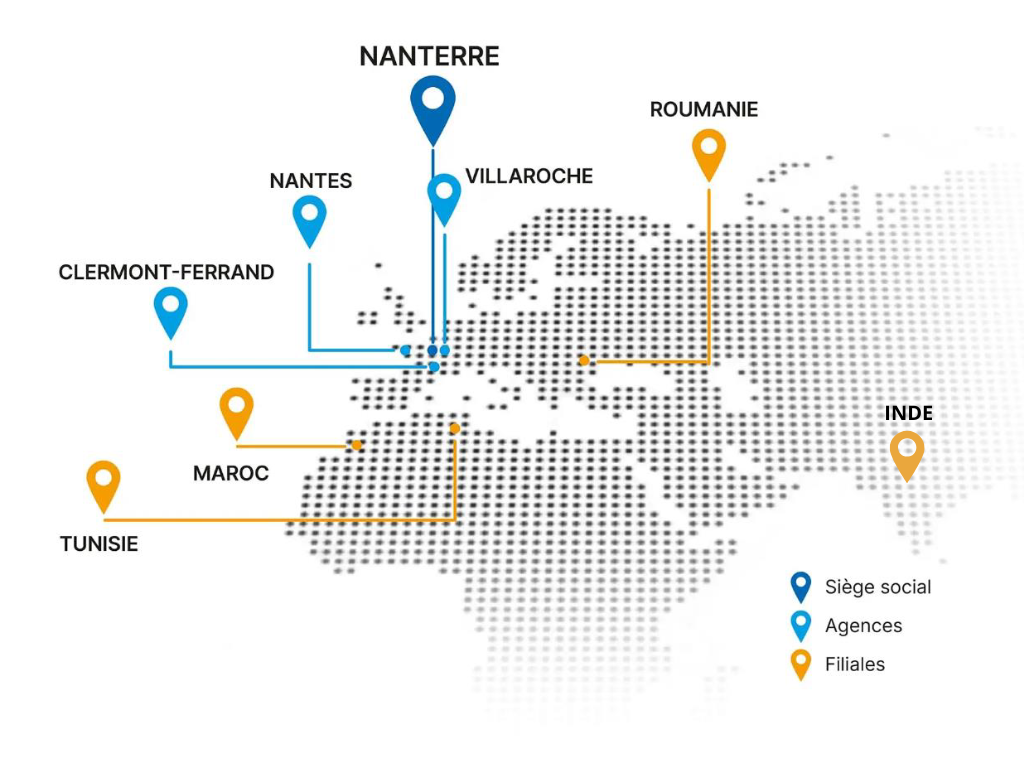
\includegraphics[width=1\linewidth]{Corps_rapport/sherpa.png}
    \captionof{figure}{Carte des agences de SHERPA Engineering dans le monde}
    \label{fig1}
\end{center}
$\ $\\
Elle est divisée en 3 Poles de direction:\\
\begin{itemize}
\renewcommand{\labelitemi}{$\bullet$}
    \item Direction Administrative et Financière
    \item Direction de l'Ingénierie
    \item Direction Stratégique\\
\end{itemize} 
Voici l'organigramme (\hyperref[fig2]{Figure 2}) de l'entreprise afin de mieux comprendre la structure.
\begin{center}
    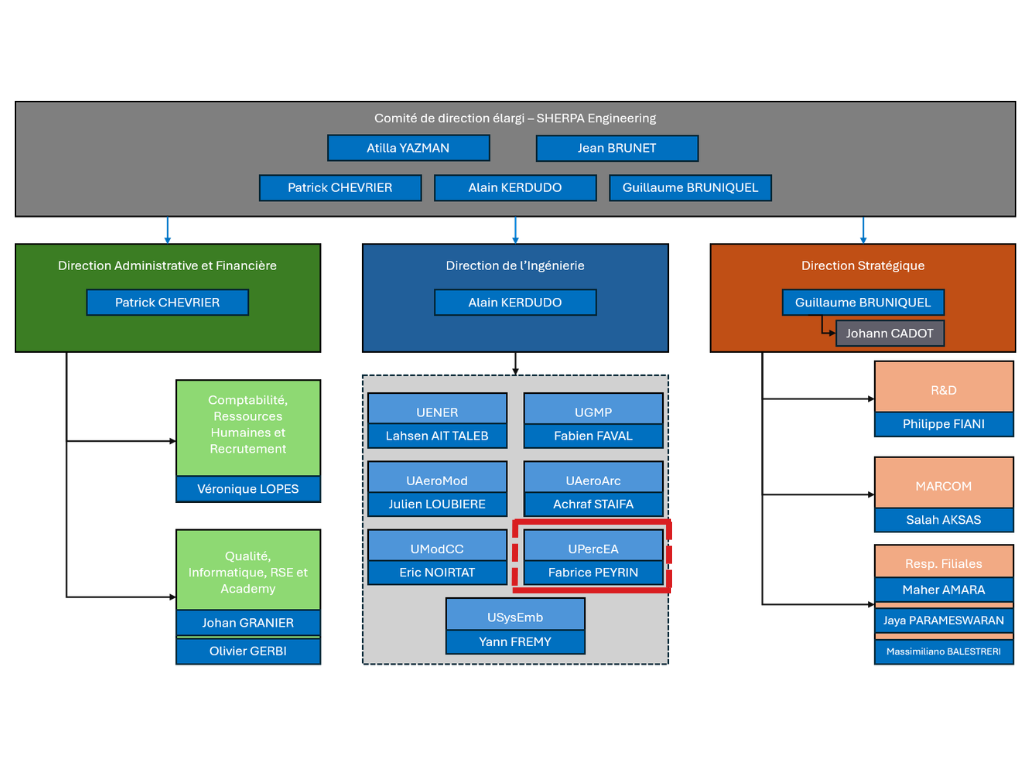
\includegraphics[width=1\linewidth]{Corps_rapport/Organigramme_SHERPA.png}
    \captionof{figure}{Organigramme de SHERPA Engineering}
    \label{fig2}
\end{center}
$\ $\\
\indent Au coeur de cette organisation, je fais partie de l'équipe UPercEA, dirigée par Fabrice PEYRIN. Cette équipe est partagée entre l'agence de Clermont-Ferrand et celle de Nantes. Mon tuteur de stage est Thomas Barbier, ingénieur en robotique spécialisé en vision artificielle.

\newpage
\section{Présentation du Challenge MOBILEX}
Comme mentionné précédemment, le Challenge MOBILEX* vise à accélérer la recherche et à faire mûrir technologiquement le domaine de la navigation autonome des véhicules en Environnement complexe*.\\\\
\indent Pour ce faire, les organisateurs ont lancé un appel à projet auquel pouvaient candidater des consortiums composés d'au moins un acteur industriel et d'un acteur de la recherche française. L'objectif était de rendre un véhicule imposé autonome pour des cas de situations donnés et de proposer des fonctionnalités/aides facilitants le contrôle par un téléopérateur.\\\\
\indent À l'issue de l'appel à projets, sept consortiums ont été retenus comme ci-après (Figure \ref{fig3}) :

\begin{figure}[H] % Utilisez [H] au lieu de [htb]
  \centering % Utilisez \centering au lieu de \makebox
  
\includegraphics[trim={0.0cm 1cm 0.0cm 2cm}, clip, width=1.05\linewidth]{Corps_rapport/Liste_consortiums.png}
  \caption{Liste des équipes du challenge}
  \label{fig3}
\end{figure}

\subsection{Le consortium MOBITER}
Pour répondre au mieux aux ambitions du Challenge MOBILEX*, SHERPA Engineering s'est associée avec ses partenaires académiques INRAE et Institut Pascal, avec lesquels elle collabore régulièrement grâce à une proximité géographique, un laboratoire qui était jusqu'à récemment commun pour SHERPA Engineering et l'Institut Pascal, et des propositions régulières de thèses CIFRE.\\\\
\indent Cette proximité permet de répartir aisément les tâches à réaliser en fonction de l'expertise de chacun et de faciliter la communication entre les différents acteurs, notamment grâce à un canal Teams sur lequel sont partagés les avancées et différents documents et où une réunion hebdomadaire a lieu, permettant de présenter le travail de chacun et de planifier les tests sur le terrain. Les apports de chaque partie sont les suivants :

\subsubsection{SHERPA Engineering}
SHERPA Engineering, coordinatrice du projet, réalise, sur la base d'un existant, la mise en place de la base hardware du projet en l'adaptant pour répondre aux exigences du challenge. Elle réalise les tâches d'ingénierie du projet et a la charge d'une partie de l'algorithmie liée à la perception et à la planification.

\subsubsection{INRAE}
L'INRAE apporte son expérience dans la robotique agricole, notamment sur les nouvelles lois de commande, et est responsable de l'expérimentation grâce à l'utilisation de ses sites à Aubière (Puy-de-Dôme) et Montoldre (Allier).

\subsubsection{Institut Pascal}
L'Institut Pascal fournit des conseils sur le développement scientifique (fusion de données, traversabilité, gestion des risques, planification) qui sont mis en application par une ressource interne.



\subsection{Les attendus du challenge}
\subsubsection{Organisation générale}
Le Challenge Mobilex* est organisé par les acteurs suivants (Figure \ref{fig4}) :

\begin{figure}[H] % Utilisez [H] au lieu de [htb]
  \centering % Utilisez \centering au lieu de \makebox
  
\includegraphics[width=1.05\linewidth]{Corps_rapport/Organisateurs_challenge_mobilex.png}
  \caption{Organisateur du challenge Mobilex}
  \label{fig4}
\end{figure}

\indent Il se déroule sur trois années et est composé de trois défis de difficulté croissante, à savoir un défi par annnée. Les modalités de ces défis ne sont communiquées aux équipes qu'au début de chaque défi \cite{anr2023mobilex}. À la fin de chaque année, toutes les équipes sont convoquées sur un site de la DGA pour y être évaluées sur leurs propositions en réponse aux situations rencontrées lors du défi.\\\\
\indent L'organisation de chaque défi se déroule comme suit (Figure \ref{fig5}) :

\begin{figure}[H] % Utilisez [H] au lieu de [htb]
  \centering % Utilisez \centering au lieu de \makebox
  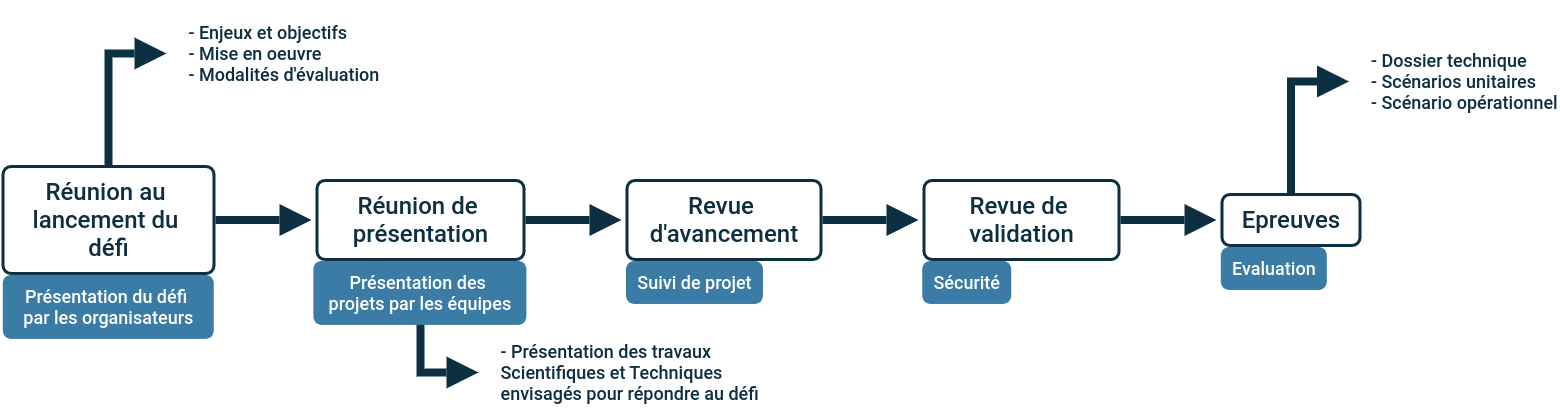
\includegraphics[width=1.05\linewidth]{Corps_rapport/timeline_defi.png}
  \caption{Déroulement d'un défi}
  \label{fig5}
\end{figure}

\subsubsection{Fonctions attendues}
Pour chaque défi, une liste de nouvelles fonctions attendues est donnée. Les fonctions demandées lors des précédents défis doivent également fonctionner lors des scénarios du défi en cours (sauf indication contraire de la DGA). Ces fonctions peuvent être classées selon deux modes de fonctionnement : le mode pilote automatique et le mode téléopération assistée.

\paragraph{Mode pilote automatique}
Pour le premier défi, les fonctions attendues étaient les suivantes :\\
\begin{itemize}
\renewcommand{\labelitemi}{$\bullet$}
    \item Détection et gestion locale des obstacles positifs franchissables et non franchissables.
    \item Détection et gestion locale des bas-côtés positifs.
    \item Fonction rejeu de trajectoire.
    \item Fonction retour sur trace.
    \item Évitement de zones d'exclusion, d'interdiction et passage par des points de passage imposés.\\
\end{itemize}

Le second défi a quant à lui demandé l'ajout des fonctions suivantes :\\
\begin{itemize}
\renewcommand{\labelitemi}{$\bullet$}
    \item Détection et gestion locale des obstacles négatifs franchissables et non franchissables.
    \item Détection et gestion locale des obstacles transparents/réflichissants.
    \item Détection et gestion locale des bas-côtés négatifs.
    \item Prise en compte des pentes positives et négatives.
    \item Détection et gestion locale des dévers.
    \item Gestion des situations dégradées (pannes capteurs, perte de communication avec le poste de téléoperation, ...).\\
\end{itemize}

Lors du troisième et dernier défi, les équipes se sont vu supprimer certaines fonctions imposées au cours des précédents défis, à savoir :\\
\begin{itemize}
\renewcommand{\labelitemi}{$\bullet$}
    \item Le rejeu de trajectoire et le retour sur trace.
    \item Détection et gestion locale des obstacles transparents/réflichissants.
    \item Détection et gestion locale des obstacles à bascules.
    \item Le changement artificiel de gabarit.
    \item Gestion des pannes capteurs. \\
\end{itemize}

Et se sont vu rajouter les nouvelles fonctions suivantes :\\
\begin{itemize}
\renewcommand{\labelitemi}{$\bullet$}
    \item Gestion des pentes et dévers avec obstacles franchissables ou non.
    \item Gestion de la végétation et des flaques d'eau.
    \item Suivi de bas-côtés (positif et négatif) avec gestion d'obstacles sur la trajectoire.
    \item Gestion des situations dégradées (perte des donnés gnss, perte de communication avec le poste de téléoperation, ...).
\end{itemize}


\paragraph{Mode téléopération assistée}
Pour le premier défi, une IHM fonctionnant sur un PC déporté a été demandée pour, au minimum, pouvoir choisir le mode de pilotage, renvoyer les commandes réalisées par le téléopérateur lors d'un pilotage manuel et fournir un retour vidéo annoté. Ce retour vidéo doit contenir des informations concernant la compréhension de l'environnement établie par la brique logicielle de l'équipe ainsi que les indications de direction pour gérer la trajectoire.\\\\
\indent Lors du défi 2, un sous-mode \textit{Safety First} en téléopération assistée a été demandé. Ce mode vise à préserver l'intégrité du robot en imposant le respect des contraintes de navigation données par les organisateurs, en reprenant temporairement le contrôle du véhicule en cas de danger. Ce sous-mode doit être activable ou désactivable à tout moment depuis l'IHM.

\subsubsection{Contraintes de navigation à intégrer lors du développement}

\paragraph{Détection et gestion des obstacles}
En premier lieu, la navigabilité du véhicule repose sur la classification géométrique des obstacles rencontrés sur le terrain. Tout obstacle d'une hauteur ou d'une profondeur supérieure à 30~cm par rapport au sol est considéré comme non franchissable et impose un contournement. Le franchissement d'obstacles d'amplitude intermédiaire (entre 5 et 30~cm) est quant à lui conditionné par des limitations de vitesse strictes, nécessitant parfois un arrêt préalable (Figure~\ref{fig6}).

\begin{figure}[h!]
\centering
\begin{tabular}{|>{\columncolor{blue!30}}c|c|c|c|}
\hline
\rowcolor{blue!30} & avec arrêt & $<5$ km/h & $>5$ km/h \\
\hline
$<5$ cm & \textcolor{green!70!black}{Franchissable} & \textcolor{green!70!black}{Franchissable} & \textcolor{green!70!black}{Franchissable} \\
\hline
entre 5 cm et 15 cm & \textcolor{green!70!black}{Franchissable} & \textcolor{green!70!black}{Franchissable} & \textcolor{red}{Non franchissable} \\
\hline
entre 15 cm et 30 cm & \textcolor{green!70!black}{Franchissable} & \textcolor{red}{Non franchissable} & \textcolor{red}{Non franchissable} \\
\hline
$>30$ cm & \textcolor{red}{Non franchissable} & \textcolor{red}{Non franchissable} & \textcolor{red}{Non franchissable} \\
\hline
\end{tabular}
\caption{Gestion des obstacles en fonction de leur hauteur/profondeur et de la vitesse du robot}
\label{fig6}
\end{figure}

\paragraph{Détection et gestion des bas-côtés}
Au-delà des obstacles isolés, cette logique de franchissabilité s'applique directement à la détection continue de l'environnement périphérique. Ainsi, les bas-côtés (haies, murs, fossés, barrières, lisières) d'une hauteur supérieure à 30~cm (positive ou négative) doivent être détectés en permanence, quel que soit le mode de pilotage. La fonction de suivi de bas-côté impose au robot de maintenir une distance latérale consigne tout en adaptant dynamiquement sa trajectoire face aux obstacles (franchissables ou non) s'interposant sur son passage.

\paragraph{Détection et gestion des pentes et dévers avec obstacles}
Aux contraintes dimensionnelles des obstacles et des bas-côtés s'ajoutent les contraintes topologiques du relief. Les pentes (inclinaisons longitudinales dans l'axe de progression) et les dévers (inclinaisons transversales) supérieurs à 20° sont considérés comme hors du domaine de franchissabilité et doivent être détectés en continu. Lorsque des obstacles se superposent à ces pentes ou dévers, les règles d'infranchissabilité et d'adaptation de la vitesse sont combinées selon la logique récapitulée en Figure~\ref{fig7}.

\begin{figure}[H]
  \centering
  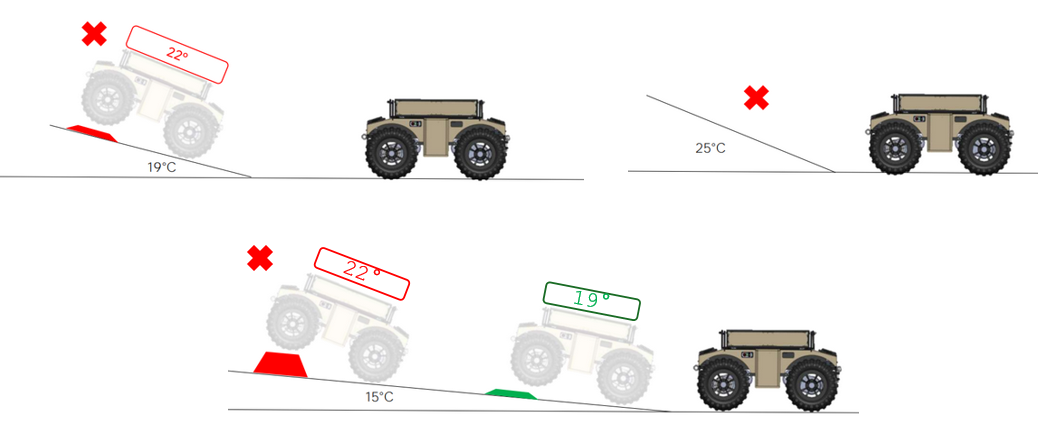
\includegraphics[width=1.05\linewidth]{Corps_rapport/Gestion_pentes.png}
  \caption{Gestion des pentes et dévers avec obstacles}
  \label{fig7}
\end{figure}

\paragraph{Gestion des situations dégradées}
Outre les contraintes physiques du terrain, le système doit garantir sa robustesse face aux perturbations environnementales et opérationnelles. Alors que le Défi~2 mettait l'accent sur la résistance aux intempéries (pluie, brouillard, fumée), le Défi~3 éprouve la capacité de la Brique MOBILEX* à maintenir l'ensemble de ses fonctions nominales en cas de couverture GNSS dégradée ou de perte de communication avec la station de contrôle débarquée.

\paragraph{Gestion des pannes capteurs}
Dans cette même optique de résilience, la brique logicielle doit tolérer des pannes matérielles transitoires (pannes brèves $< 10\text{~s}$ ou prolongées $< 2\text{~min}$) affectant individuellement le GPS, la caméra ou le LiDAR*. Bien que l'évaluation formelle de cette injection de pannes ne soit plus reconduite lors du Défi~3, cette exigence d'architecture demeure un pilier de la conception logicielle.

\paragraph{Points de passage imposés}
En complément de l'évitement d'obstacles et du suivi du relief, la trajectoire du robot est encadrée par des consignes de mission strictes. L'IHM doit permettre au téléopérateur de renseigner des points de passage imposés par les organisateurs. Le robot a pour obligation d'atteindre chacun de ces points selon l'ordre établi. Leurs coordonnées géographiques sont transmises sous forme de points cartésiens (projection UTM 31 dans le système géodésique WGS 84) avec une précision décimétrique.

\paragraph{Rejeu de trajectoire}
Sur la base de ces points de passage et des parcours enregistrés, le système propose des fonctionnalités avancées de renavigation. La Brique MOBILEX* doit pouvoir enregistrer et rejouer en autonomie n'importe quelle trajectoire préalable, quel que soit le mode de pilotage initial. Ce rejeu nécessite au préalable le repositionnement du robot au point de départ et doit adapter la trajectoire enregistrée en temps réel en cas d'apparition ou de modification d'obstacles. De plus, une option d'optimisation temporelle permet de réduire la durée de parcours tout en garantissant le franchissement ordonné des points de passage imposés.

\paragraph{Retour sur traces}
Répondant à une problématique complémentaire au rejeu, le retour sur traces permet au robot de regagner de manière autonome son point de départ (ou un point intermédiaire spécifié) en reprenant en sens inverse la trajectoire exactement parcourue à l'aller. Cette fonction, susceptible d'être déclenchée dans un contexte d'urgence, adapte sa planification face aux nouveaux obstacles et peut déroger aux limitations de vitesse nominales. Elle offre la flexibilité d'être exécutée en marche avant comme en marche arrière, avec changement de sens dynamique.

\paragraph{Zones d'exclusion}
Enfin, l'ensemble des algorithmes de planification de trajectoire (qu'il s'agisse du suivi de lisière, du rejeu ou du retour sur traces) doit intégrer des contraintes d'espace strictes définies par l'organisation. Les zones d'exclusion sont des polygones géographiques (coordonnées UTM 31) représentant des emprises interdites, pas nécessairement matérialisées sur le terrain. Tout franchissement de ces zones, tout comme la prise en compte erronée d'une zone virtuelle inexistante entraîne des pénalités au classement.

\paragraph{Zones d'interdiction}
Distinctes des zones d'exclusion par leur niveau de criticité, les zones d'interdiction constituent des enveloppes de sécurité absolue. Également définies sous forme de polygones géographiques (coordonnées UTM 31) virtuels, leur moindre chevauchement déclenche immédiatement un arrêt d'urgence du véhicule ainsi qu'une pénalité lourde, primant sur toutes les autres consignes de navigation.

\subsubsection{Évaluation des développements pour le défi en cours.}
L'évaluation des développements se fait à chaque défi et comporte trois notes : une note liée à la revue de validation, une note liée à la soumission du dossier scientifique et technique et une note liée aux épreuves. Elles visent à démontrer les capacités de développement de l'équipe et les performances du système développé.\\

\indent Lors de la journée d'épreuves sur un site de la DGA, les robots des équipes doivent accomplir une suite de scénarios donnés dans le règlement particulier du défi permettant d'évaluer des fonctions seules ou un ensemble de fonctions. Les équipes sont notées sur la bonne prise en compte de l'ensemble des contraintes fournies par les organisateurs et le bon fonctionnement des fonctions avec des critères de précision et/ou de rapidité.


\subsection{Présentation du robot BARAKUDA et des équipements embarqués}

\subsubsection{Plateforme robotique BARAKUDA}
Afin d'assurer la cohérence des évaluations entre les candidats, la DGA a fourni à chaque équipe le robot tout-terrain BARAKUDA, conçu par la société SHARK ROBOTICS (Figure~\ref{fig8}).

\begin{figure}[H]
  \centering
  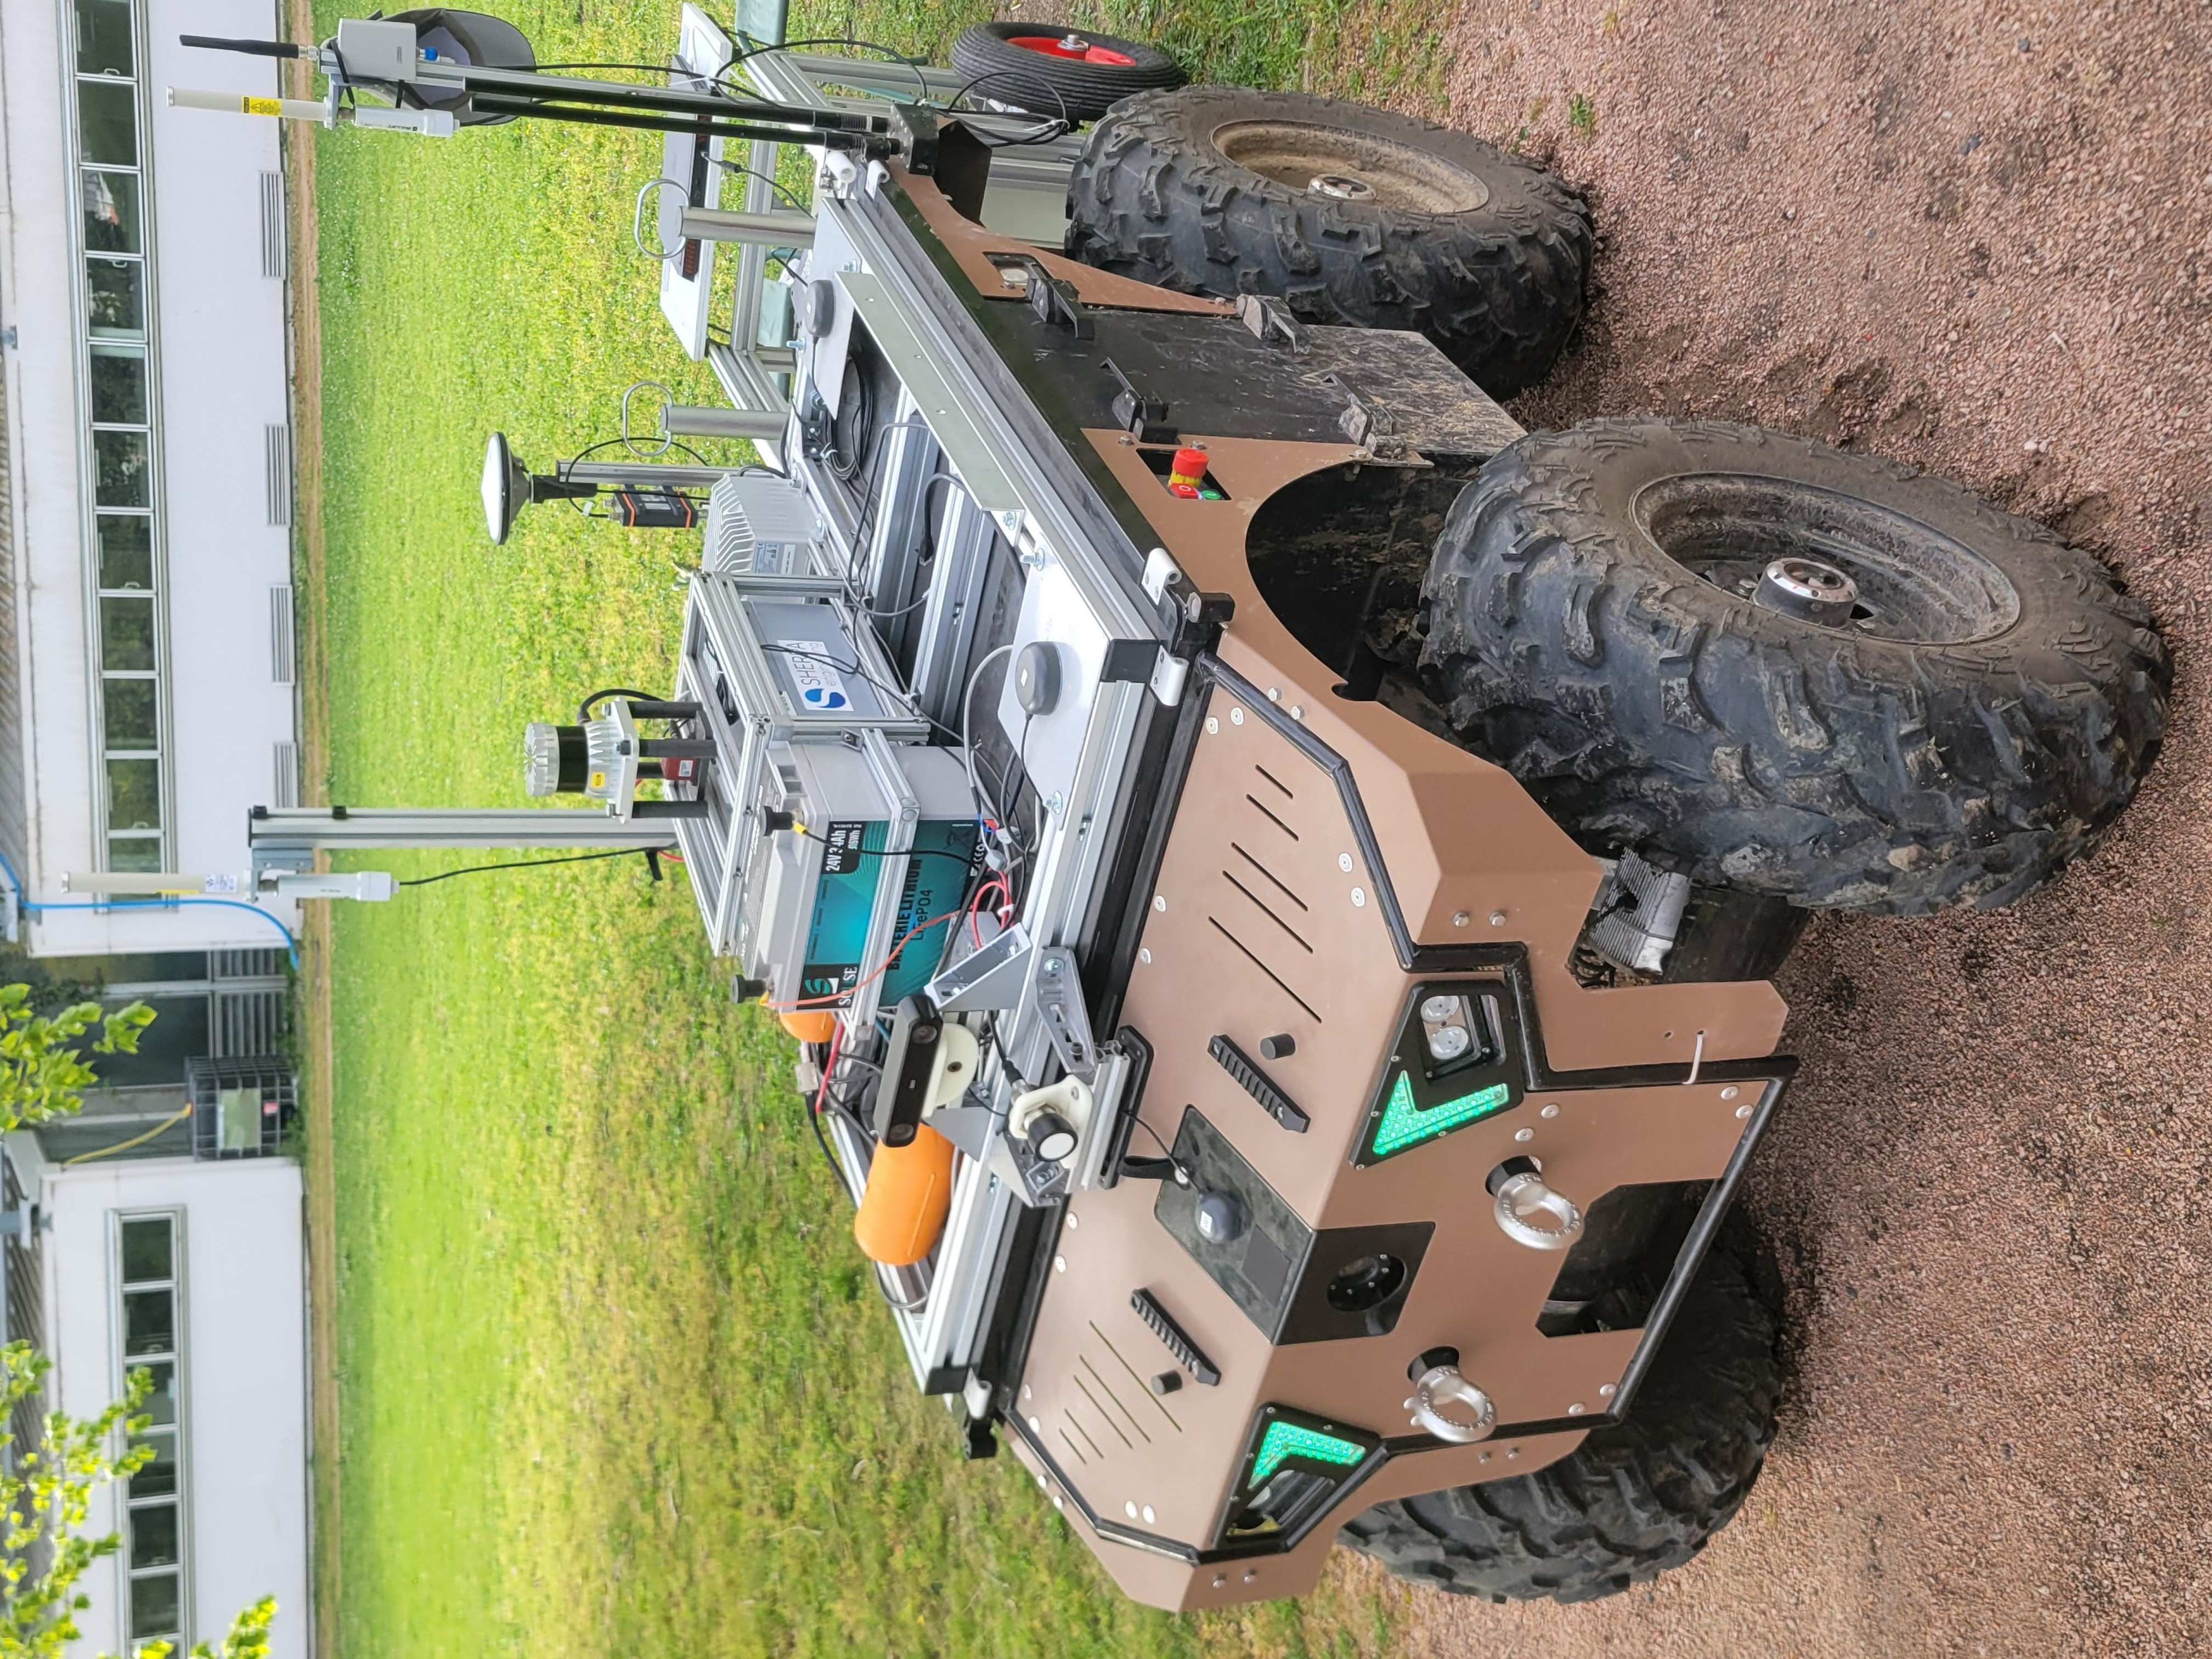
\includegraphics[width=0.5\linewidth, angle=-90]{Corps_rapport/barakuda.jpg}
  \caption{Plateforme mobile BARAKUDA (SHARK ROBOTICS)}
  \label{fig8}
\end{figure}

Il s'agit d'une plateforme chenillée à quatre roues motorisées non directionnelles d'une masse à vide de 500~kg, téléopérable jusqu'à une portée de 500 mètres en champ libre à l'aide de sa radiocommande d'origine. Capable de transporter une charge utile maximale de 500~kg, la plateforme atteint une vitesse de pointe de 20~km/h, franchit des obstacles d'une hauteur maximale de 30~cm et évolue sur des pentes jusqu'à 40° ainsi que des dévers jusqu'à 35°. En conditions opérationnelles, son autonomie atteint jusqu'à 10 heures.\\\\
\indent L'interface de communication entre le calculateur de bord et la Brique MOBILEX* s'appuie sur le protocole UDP (User Datagram Protocol). Ce choix garantit un traitement à très faible latence au détriment du contrôle d'acquittement, privilégiant ainsi l'actualité des données rafraîchies à haute fréquence. L'échange de données s'effectue via des trames structurées permettant d'envoyer les consignes de vitesse (linéaire et angulaire) et de collecter, par requêtes de type \texttt{GET}, l'état de santé du robot (vitesse et puissance moteur de chaque roue, inclinaisons attitude/cap, niveau de batterie et températures).

\subsubsection{Suite sensorielle et architecture matérielle ajoutées par le consortium}
Bien qu'il soit interdit de modifier la structure mécanique du robot, les équipes sont libres d'embarquer des équipements matériels dans la limite de la charge utile et du gabarit imposés. Le consortium MOBITER a ainsi équipé le robot avec les composants décrits ci-après (Figure~\ref{fig9}) :

\begin{figure}[H]
  \centering
  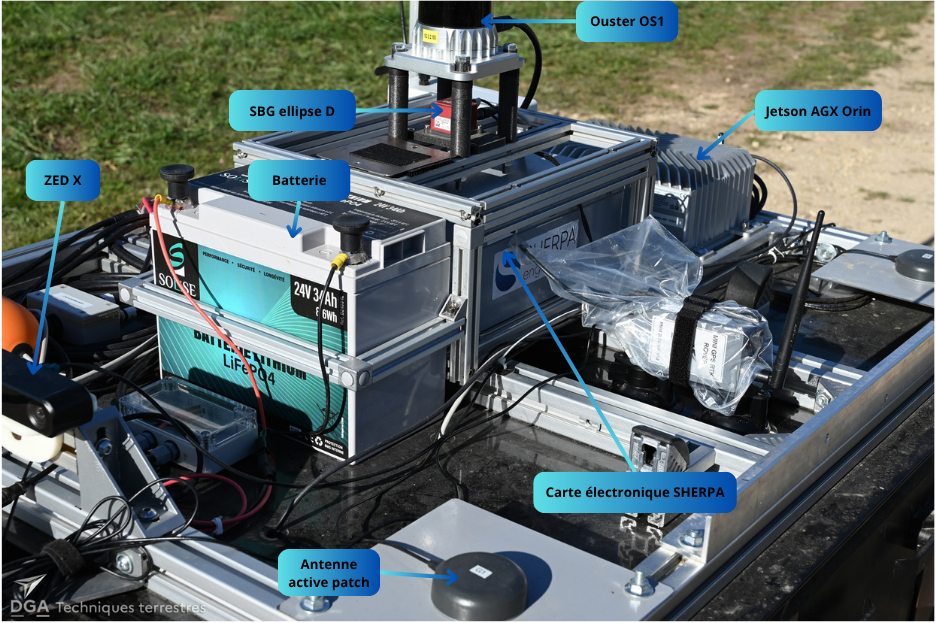
\includegraphics[width=0.7\linewidth]{Corps_rapport/Plateau_hardware.png}
  \caption{Implantation du plateau capteurs et des calculateurs embarqués}
  \label{fig9}
\end{figure}

\paragraph{Calculateur industriel Syslogic RML A4AGX}
%Afin d'absorber la charge de calcul engendrée par les nouvelles algorithmiques de perception et de planification, l'ancien calculateur Syslogic RML A3 a été remplacé par le modèle RML A4AGX. 
Ce calculateur industriel renforcé, à dissipation thermique passive, intègre un System-on-Module (SoM) NVIDIA Jetson AGX Orin. Il s'appuie sur un processeur ARM Cortex-A78AE à 12 cœurs (2,2~GHz), un GPU NVIDIA Ampere de 2048 cœurs CUDA, 64~Go de RAM LPDDR5 et des accélérateurs d'inférence deep learning NVIDIA DLA. Il dispose en outre de 6 contrôleurs Gigabit Ethernet indépendants et de 2 ports USB 3.1. Un SSD NVMe PCIe de 2~To a été ajouté en interne pour l'enregistrement à haute fréquence des données de logs (\emph{rosbags}). Ce composant a été retenu pour son excellente efficacité énergétique (ratio performance/Watt) et ses capacités de calcul parallèle adaptées à des applications robotiques et embarquées exigeantes.

\paragraph{Système de navigation inertielle (INS) SBG Ellipse-D}
Positionné au centre géométrique du plateau capteurs, ce système de navigation inertielle permet d'estimer en temps réel la pose 3D (position et orientation) ainsi que les vitesses linéaires et angulaires du robot. Il intègre une centrale inertielle (IMU) triaxiale étalonnée et compensée en température, couplée à un récepteur GNSS RTK double antenne permettant une estimation précise du cap même à l'arrêt. La fusion des données sensorielle est réalisée en interne par un filtre de Kalman étendu (EKF). Son choix repose sur sa compacité, son niveau de précision et sa robustesse mécanique.

\paragraph{LiDAR 3D Ouster OS1}
Installé en position haute au-dessus du système INS pour dégager son champ de vue, ce LiDAR 3D à 64 nappes assure une perception volumétrique de l'environnement à 360°. Retenu pour sa compacité et sa résilience mécanique face aux vibrations, il constitue le capteur maître de la chaîne de perception et de cartographie.

\paragraph{Caméra stéréoscopique ZED X}
Disposée à l'avant du véhicule, cette caméra stéréo fournit un retour vidéo haute définition pour la téléopération, tout en générant un nuage de points 3D dense sur le secteur avant. Ses données sont fusionnées avec celles du LiDAR 3D pour combler les zones d'ombre à courte portée et alimenter les algorithmes de segmentation sémantique d'images par réseau de neurones.

\paragraph{Sous-système électronique et d'acquisition SHERPA}
Conçu sur mesure par SHERPA Engineering, ce boîtier étanche (IP67) intègre des cartes électroniques dédiées à la synchronisation temporelle matériel, au pilotage sécurisé et au multiplexage des bus de données capteurs. Il embarque une centrale inertielle XSens MTi-7 couplée à un module GNSS u-blox ZED-F9P, offrant une redondance matérielle complète vis-à-vis du système SBG Ellipse-D.

\paragraph{Liaisons RF (Antennes 5~GHz et 868~MHz)}
Dans le cadre du défi 3, la communication hertzienne entre le poste de contrôle et le robot s'appuie sur la liaison 5~GHz. Bien que deux paires d'antennes (5~GHz et 868~MHz) équipent le système, la liaison 5~GHz a été privilégiée pour sa bande passante élevée et sa plus grande robustesse aux obstacles (végétation, bâtiments, ...).

\paragraph{Poste de Contrôle-Commande (PCC / Station sol)}
Le poste débarqué (Figure~\ref{fig10}) est constitué d'un PC portable durci, d'un jeu d'antennes omnidirectionnelles, d'une interface de pilotage type manette et d'un sous-système d'alimentation secouru par onduleur. Il permet à l'opérateur d'assurer le pilotage à distance, la supervision de l'état du système et la configuration des missions.

\begin{figure}[H]
  \centering
  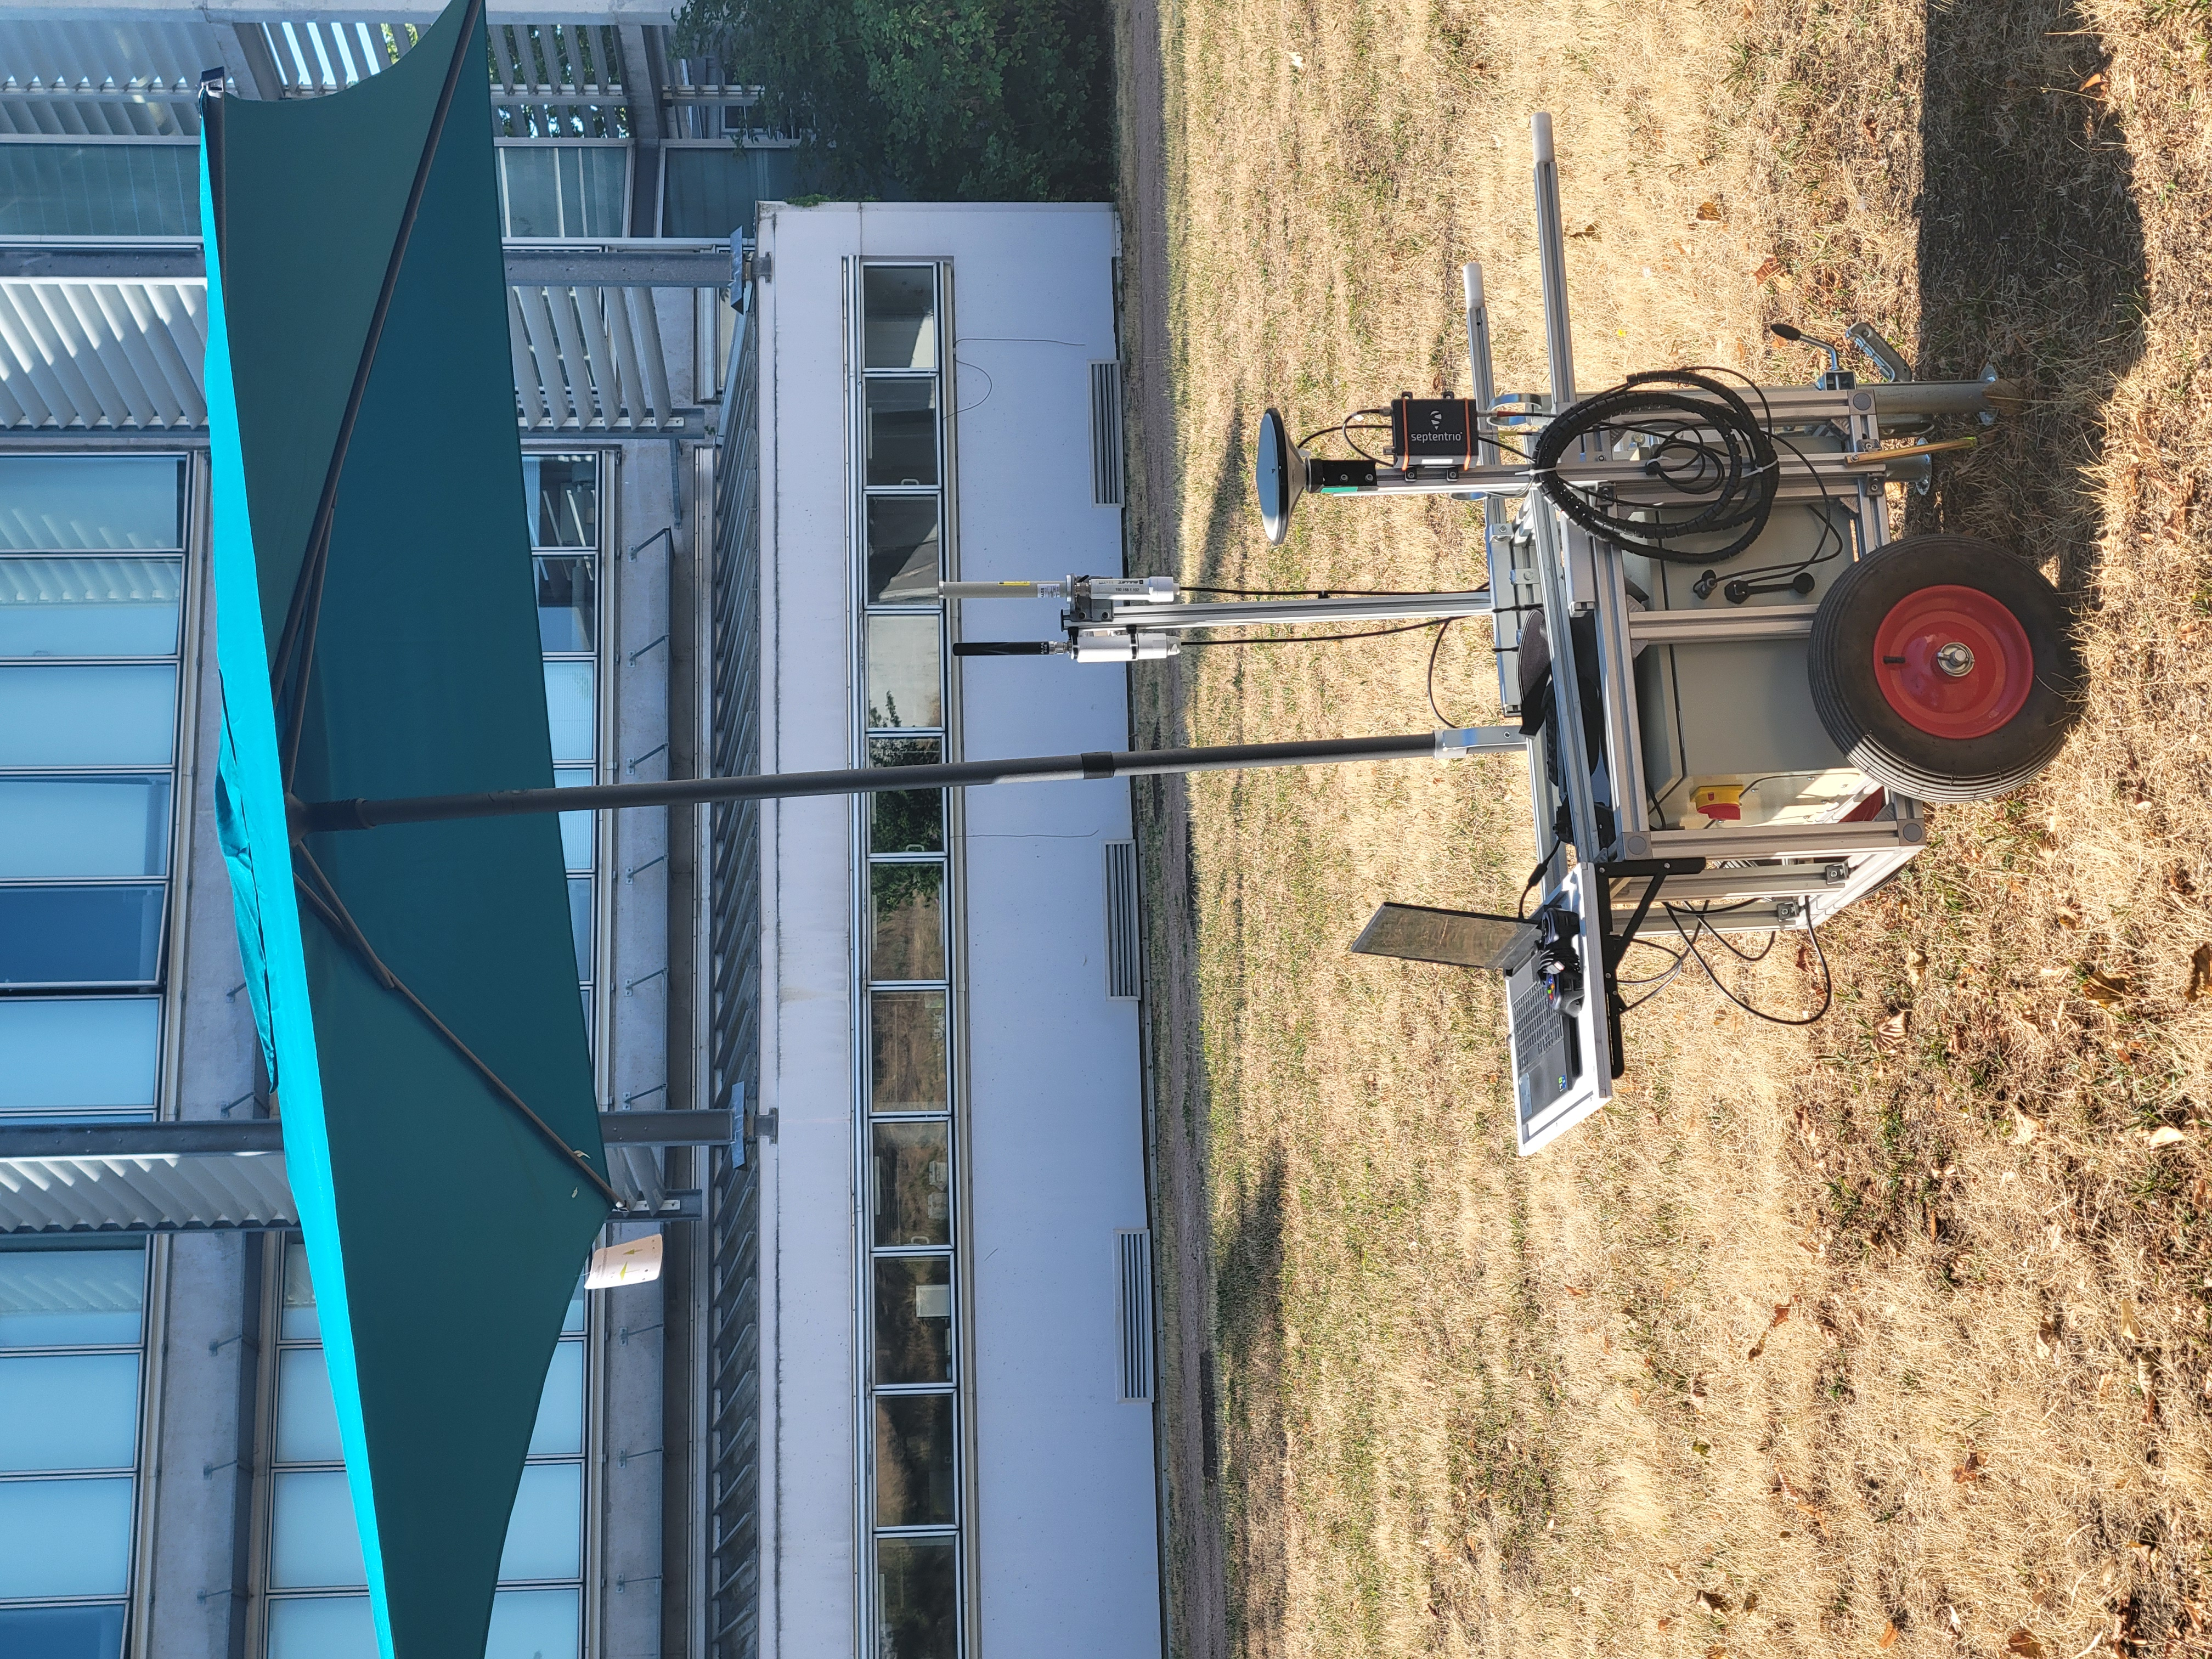
\includegraphics[width=0.5\linewidth, angle=-90]{Corps_rapport/PCC.jpg}
  \caption{Poste de Contrôle-Commande (PCC) débarqué}
  \label{fig10}
\end{figure}

L'ensemble de ces sous-systèmes s'articule selon l'architecture matérielle globale présentée sur la Figure~\ref{fig11} :

\begin{figure}[H]
  \centering
  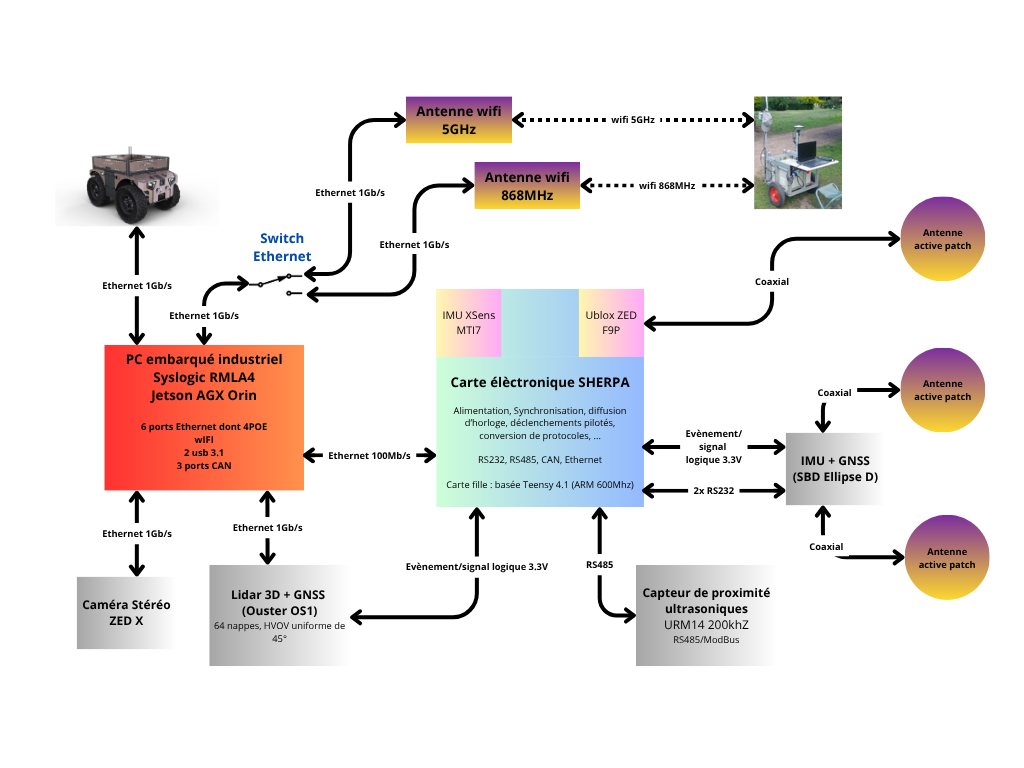
\includegraphics[trim={0.0cm 2cm 0.0cm 2cm}, clip, width=1\linewidth]{Corps_rapport/Architecture_système.png}
  \caption{Diagramme synoptique de l'architecture matérielle embarquée}
  \label{fig11}
\end{figure}

\subsection{Environnement de simulation Gazebo}
Afin de sécuriser les phases de développement et conformément aux méthodologies de validation logicielle en boucle ouverte/fermée, SHERPA Engineering a conçu un environnement de simulation sous Gazebo (Figure~\ref{fig12}). Ce jumeau numérique réplique fidèlement les interfaces d'entrées/sorties du robot ainsi que l'ensemble des flux capteurs (cf. graphe RQT en annexe~\hyperref[annexe1]{[I]}).\\\\
\indent Cette étape de simulation permet de valider le comportement des briques haut niveau (perception, cartographie, planification A* / DWA et génération de commandes) avant les essais sur plateforme réelle. L'environnement virtuel intègre des reliefs complexes, de la végétation et divers obstacles représentatifs des cahiers des charges de la DGA, et évolue au rythme des exigences des différents défis du challenge.

\begin{figure}[H]
  \centering
  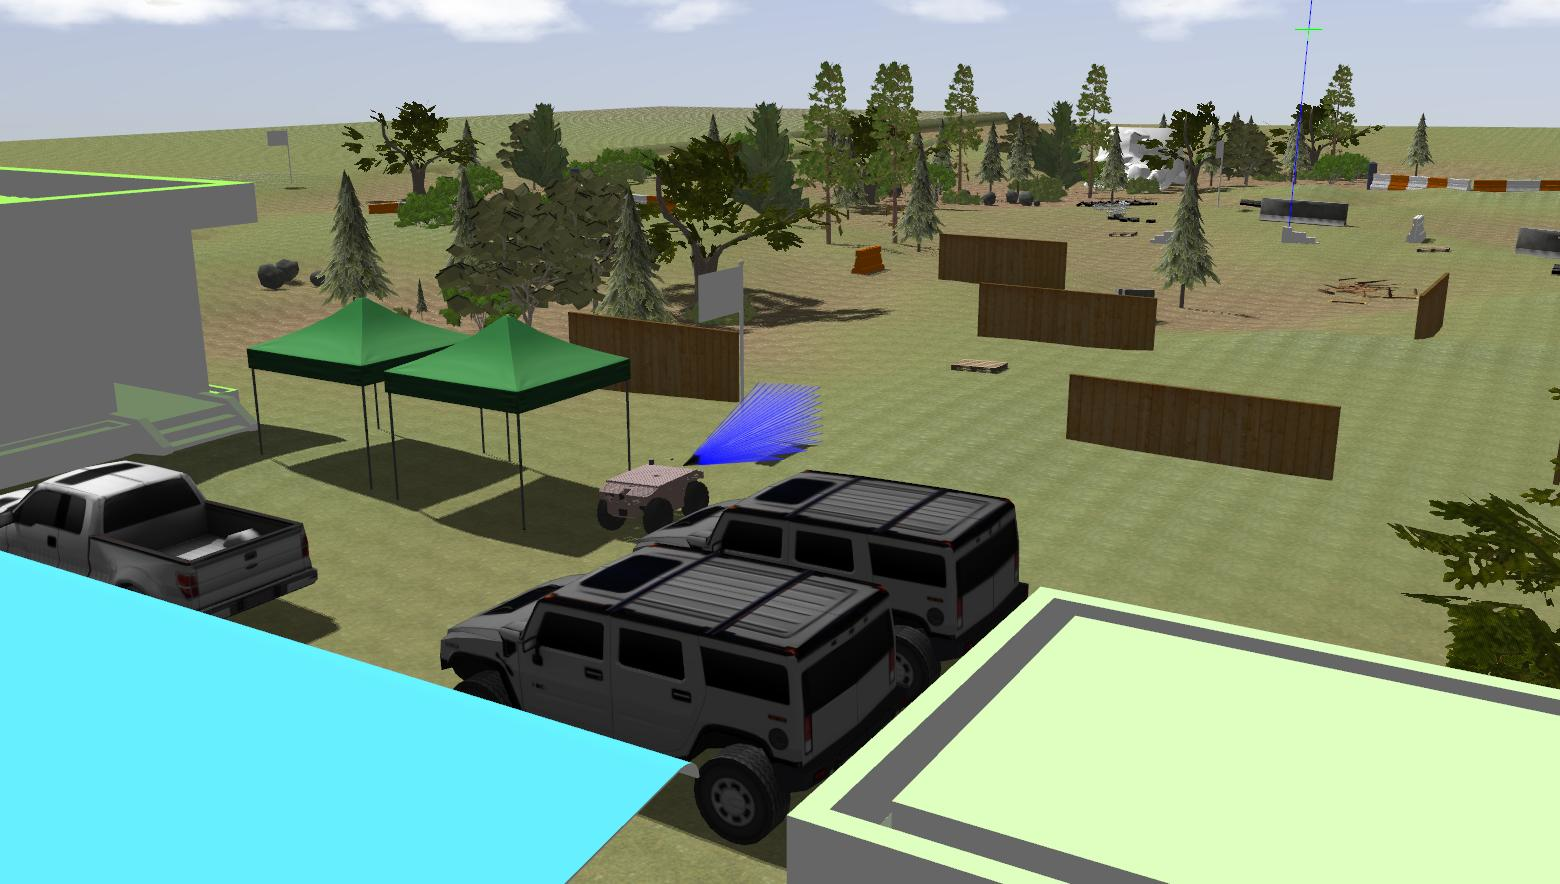
\includegraphics[width=1\linewidth]{Corps_rapport/gazebo_sim.png}
  \caption{Vue de l'environnement de simulation développé sous Gazebo}
  \label{fig12}
\end{figure}

\newpage
\section{Présentation des briques logicielles du robot}
Les développements logiciels se font sous le middleware ROS* (noetic), ce qui permet de développer sur une base standardisée offrant de nombreuses fonctionnalités et outils pour faciliter l'intégration des apports des différents acteurs à la Brique MOBILEX*. L'utilisation de ce middleware nous permet d'organiser le code comme un ensemble de briques élémentaires effectuant des fonctions bien définies prenant des données en entrées et retournant les résultats en sortie. L'assemblage de ces différentes briques constitue notre Brique MOBILEX*. Cette organisation permet si nécessaire d'ajouter, retirer ou remplacer des fonctions élémentaires sans avoir à modifier le reste des fonctions. De plus, les fonctions intensives en calcul sont développées en C++ pour répondre à des contraintes de temps réel et les autres en Python car plus rapide à développer.\\
\indent Un schéma synoptique de l'architecture du système est donné ci-dessous (Figure \ref{fig13}):\\
\begin{itemize}
\renewcommand{\labelitemi}{$\bullet$}
    \item Les modules et données de bas-niveau et hardware sont représentés en rouge.
    \item Les modules et données de perception/ localisation sont représentés en vert.
    \item Les modules et données de navigation sont représentés en bleu.
    \item Les modules et données de contrôle sont représentés en jaune.
    \item Les modules et données d’interface, de logique, de contrôle de mission ou de visualisation sont représentés en blanc.\\
\end{itemize}
\indent Il est à noter que l'ensemble des fonctions publient également des diagnostics, non représentés ici par souci de lisibilité.

\begin{center}
    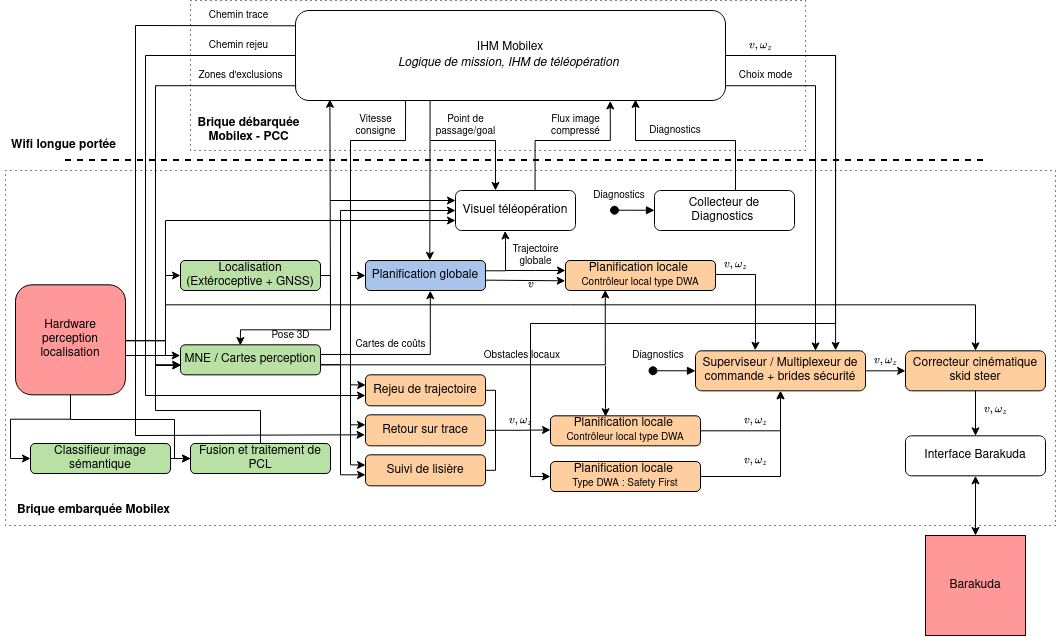
\includegraphics[width=1 \linewidth]{Corps_rapport/architecture_logicielle.png}
    \captionof{figure}{Diagramme synoptique de l'architecture logicielle du système}
    \label{fig13}
\end{center}

\subsection{Briques de perception de l'environnement}
Les briques de perception de l'environnement ont pour objectif de récolter des données provenant de capteurs majoritairement extéroceptifs pour pouvoir en concevoir une modélisation.

\subsubsection{Modèle Numérique d'Élévation}
La brique de cartographie selon un MNE (Modèle Numérique d'Élévation) se compose de deux parties : une librairie en C++ permettant de générer le MNE et un noeud ROS* permettant d'utiliser le MNE pour concevoir des cartes d'élévations correspondant aux modalités du Challenge.\\

\indent Le MNE permet de concevoir une représentation en vue de dessus de l'élévation de l'environnement sous la forme d'une carte de chaleur discrète (Figure \ref{fig14}) d'une résolution de 10x10cm. Il est construit à partir des données de position du robot, de ses vitesses 3D et des points LIDAR*. Ces données sont reçues de façon asynchrone et mises dans des tampons. Pour chaque nouvelle donnée, une partie de la carte, de 40x40m centrée autour de la position du robot, est publiée. Le MNE est mis à jour sur reception d'un scan LIDAR*, provoquant un ensemble d'interpolations pour trouver la vitesse et la position exacte du robot au moment exact du début du scan. Le nuage de points fourni par le LIDAR* est ainsi corrigé en distorsion en utilisant le début du scan comme référence et replacé dans le repère monde. Chaque point du nuage ainsi constitué sert alors à actualiser les valeurs d'élévations maximales présentes dans les tuiles de la carte grâce à un filtrage de Kalman* se servant de la position du robot et de la position des impacts LIDAR* et de leurs covariances associées.

\begin{center}
    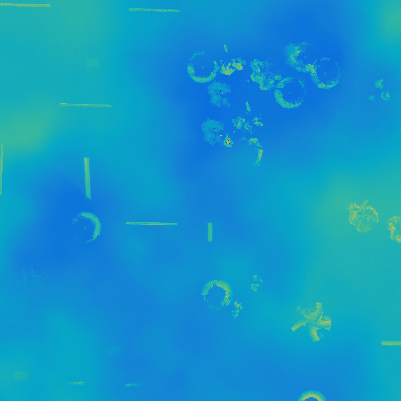
\includegraphics[width=0.4\linewidth]{Corps_rapport/MNE.png}
    \captionof{figure}{Extrait du Modèle Numérique d’Élévation sous forme d’une carte de chaleur}
    \label{fig14}
\end{center}
$\ $\

\indent Le noeud ROS* associé au MNE récupère la carte de 40x40m centrée autour du robot pour construire une carte de gradients, en utilisant un filtre de Sobel de taille 3x3 tuiles (30x30cm). Le Filtre de Sobel est un opérateur utilisé en traitement d'image pour faire de la détection de contours. Il permet de calculer le gradient d'intensité de chaque pixel ce qui indique la direction de la variation ainsi que son intensité, ce qui permet de faire ressortir les contours d'une image. En détournant cet usage sur notre carte d'élévation où la couleur nous donne une information sur la hauteur, on obtient une information sur les variations de hauteur pour chaque tuile.\\
\indent On vient ensuite seuiller notre carte de gradients afin d'obtenir une information correspondant aux différentes hauteurs d’obstacles à différencier pour le défi. La superposition de ces cartes permet d'obtenir une représentation des obstacles autour du robot comme illustré (Figure \ref{fig15}) :

\begin{center}
    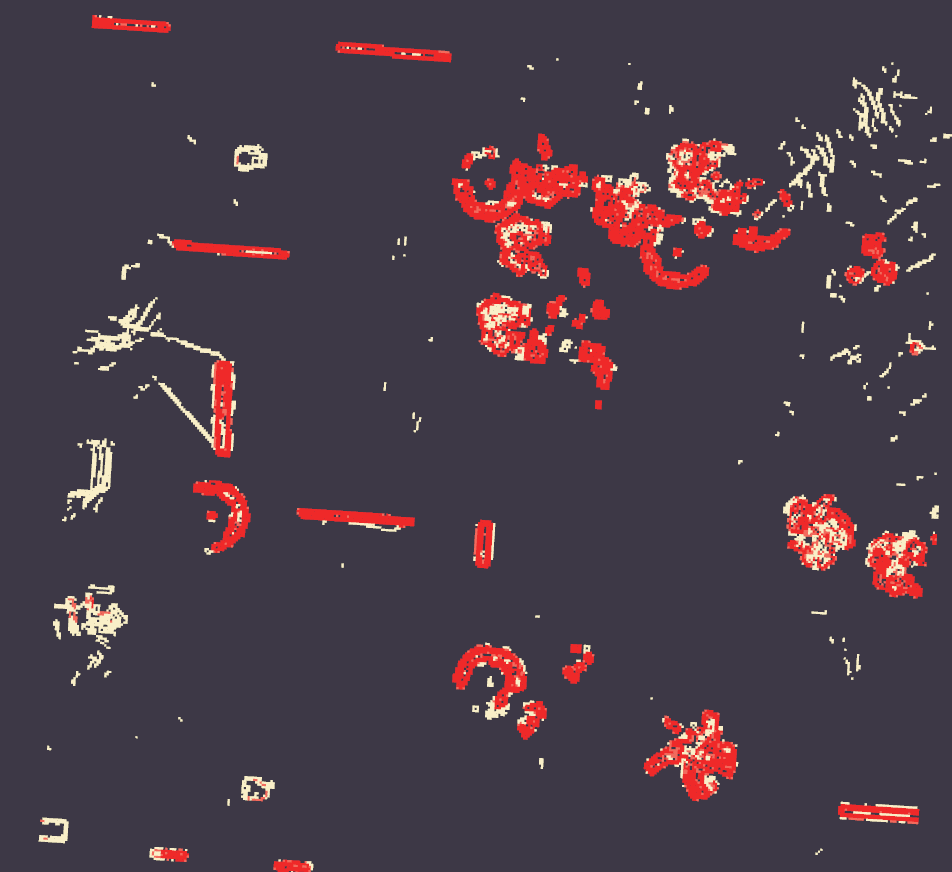
\includegraphics[width=0.4\linewidth]{Corps_rapport/Carte_obstacles.png}
    \captionof{figure}{Représentation des obstacles autour du robot}
    \label{fig15}
\end{center}
$\ $\

\indent Il est possible de demander une carte de coût associée à cette représentation selon un modèle client/serveur. Cette fonction est exploitée par le planificateur global lorsqu'il estime qu'un recalcul de la trajectoire globale est nécessaire.\\
\indent Il existe de nombreuses méthodes pour cartographier l'environnement \cite{thrun2009robotic}, permettant d'obtenir des représentations adaptées à la situation avec les capteurs disponibles \cite{lombard2020stochastic, jaspers2017multi, guerrero2015lidar}. La majorité de ces méthodes reposent néanmoins sur une fusion de données proprioceptives (odométrie, IMU) et extéroceptives (caméra, LIDAR*, ultrason, etc) avec un filtrage Kalman*.




%% verifier le maintien et la coherence de la section Segmentation d'image



\subsubsection{Segmentation d'image}
La brique de segmentation d'image* permet d'extraire des informations sémantiques à partir des images caméra. Elle a subi une modification complète par rapport aux années précédentes du défi. La combinaison des deux réseaux de neurones (détecteur open-set, YOLO World \cite{yoloworld2024} et un réseau de segmentation*, Efficient SAM \cite{efficientsam2024}) employée lors du défi 2 a été remplacée par un réseau de segmentation unique Segformer \cite{segformer}.\\


\begin{comment}
\indent Le détecteur open-set YOLO World est un réseau de neurones qui prend en entrée une image ainsi qu'un texte décrivant l'objet à détecter et à localiser. Il fournit en sortie des boîtes englobantes représentant les zones où les objets ont été détectés.\\\\
\indent Ce détecteur est dit open-set car, contrairement aux autres modèles YOLO, il est capable de détecter des objets qui ne figuraient pas dans son jeu de données d'entraînement initial. Cela est rendu possible grâce à l'intégration de techniques avancées d'apprentissage automatique et de traitement du langage naturel, permettant au modèle de comprendre et d'interpréter une large gamme d'objets à partir de descriptions textuelles.\\\\
\indent Une fois les objets détectés dans l'image, la sortie de YOLO World est utilisée comme entrée pour Efficient SAM, une version optimisée pour l'embarqué du réseau de neurones SAM \cite{segmentanything2023}. Efficient SAM se charge de segmenter précisément les objets en coloriant les pixels au sein des boîtes englobantes, ce qui nous donne le résultat (\hyperref[fig16]{Figure 16}) : \\
\begin{center}
    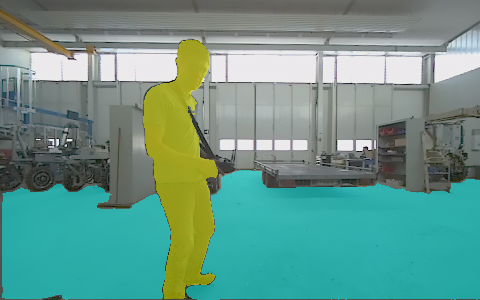
\includegraphics[width=0.8 \linewidth]{Corps_rapport/segmentation.png}
    \captionof{figure}{Résultat de la segmentation obtenu avec la combinaison de YOLO World et Efficient SAM}
    \label{fig16}
\end{center}
$\ $\

\indent Pour assurer un fonctionnement en temps réel, ces réseaux sont optimisés en supprimant les poids dont la valeur est proche de zéro, réduisant ainsi le nombre de paramètres. Cette optimisation est réalisée avec TensorRT. Une optimisation plus performante également envisagée serait d'utiliser des réseaux de neurones plus précis comme SAM et de réaliser une distillation de connaissances en entraînant un réseau de neurones constitué de moins de paramètres et spécialisé pour notre cas d'application à l'aide des sorties du réseau plus important.\\\\

\end{comment}

\indent SegFormer est une architecture de réseau de neurones dédiée à la segmentation sémantique d'images. À partir d'une image en entrée, il génère une carte de segmentation attribuant chaque pixel à une classe spécifique — dans notre cas : sol, hautes herbes et eau. Le réseau a d'abord été pré-entraîné sur le jeu de données public COCO, qui regroupe une large variété d'images annotées, puis affiné (fine-tuning) sur une base de données d'images propriétaires du groupe MOBITER. Ces données ont été acquises via la caméra ZED du robot lors de campagnes de collecte (ciblant les hautes herbes traversables et les flaques d'eau) réalisées sur les sites INRAE d'Aubière et de Montoldre.\\

\indent L'objectif est de fusionner cette information sémantique (sol, hautes herbes et eau) dans la brique du Modèle Numérique d'Environnement (MNE) pour ajouter une notion de traversabilité aux obstacles haute herbes et eau de la carte en mode dégradé. Et ainsi répondre aux exigences du défi 3.










\subsection{Briques de planification}
L'objectif des briques de planification est de calculer une trajectoire à suivre pour remplir un objectif à partir de la perception de l'environnement.

\subsubsection{Planification globale}
La brique de planification globale se sert des cartes de coûts générées par la brique du MNE pour recalculer périodiquement un chemin continu reliant le robot à un point dans le repère monde. Le chemin est obtenu par un algorithme de recherche de chemin classique de type A* \cite{hart1968formal} modifié.\\

\indent Cet algorithme est une amélioration de l'algorithme de Dijkstra \cite{dijkstra1959note} qui permet de trouver le chemin optimal selon un critère donné dans un graphe. \\

\indent Pour trouver ce chemin, l'algorithme de Dijkstra attribue à son noeud de départ un coût de 0 et attribue aux chemins vers les noeuds voisins des poids, par exemple la distance à vol d'oiseau. Le coût d'un noeud voisin correspond à la somme entre le coût du noeud précédent et le poids du chemin pour rejoindre le nouveau noeud (équation \eqref{eq1}).

\begin{equation} \label{eq1}
    c(n)=c(k)+p(k,a)
\end{equation}

où $n$ est le noeud exploré, $k$ est le noeud précédent et $a$ est l'action de déplacement utilisée depuis le noeud $k$.\\

\indent Il explore alors le noeud dont le coût est le plus faible en ajoutant les poids des chemins voisins ainsi que le coût des noeuds voisins et répète l'exploration jusqu'à atteindre l'objectif.\\

\indent La Figure \ref{fig17} est une représentation étape par étape de l'exploration d'une carte par l'algorithme de Dijkstra. Seuls les mouvements (haut, bas, gauche, droite) sont admissibles. La case bleue est le point de départ de l'algorithme, la case verte l'objectif à atteindre et le cercle jaune le noeud en cours d'exploration :

\newpage

\begin{figure}[h]
    \centering
    \begin{subfigure}[b]{0.48\textwidth}
        \centering
        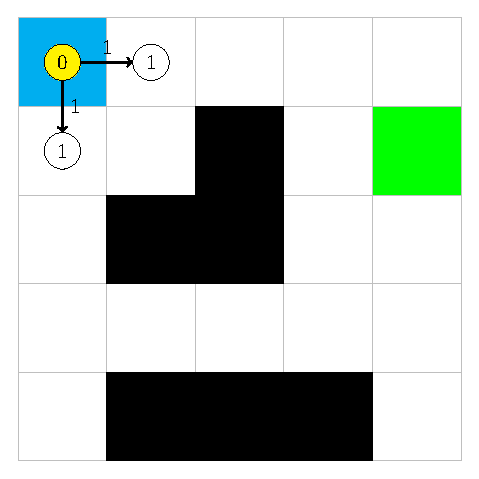
\includegraphics[width=\textwidth]{Corps_rapport/plan1.pdf}
        \caption{Exploration du noeud de départ}
        \label{fig:image1}
    \end{subfigure}
    \hfill
    \begin{subfigure}[b]{0.48\textwidth}
        \centering
        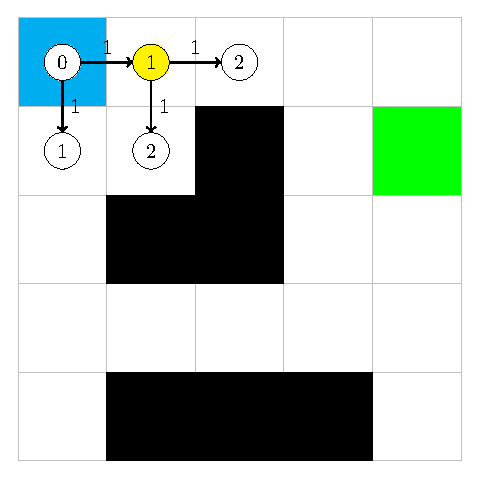
\includegraphics[width=\textwidth]{Corps_rapport/plan2.pdf}
        \caption{Exploration du noeud de coût le plus faible}
        \label{fig:image2}
    \end{subfigure}
    \vfill
    \begin{subfigure}[b]{0.48\textwidth}
        \centering
        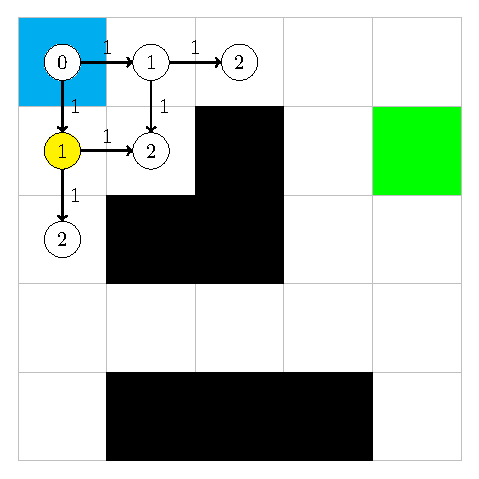
\includegraphics[width=\textwidth]{Corps_rapport/plan3.pdf}
        \caption{Nouvelle exploration}
        \label{fig:image3}
    \end{subfigure}
    \hfill
    \begin{subfigure}[b]{0.48\textwidth}
        \centering
        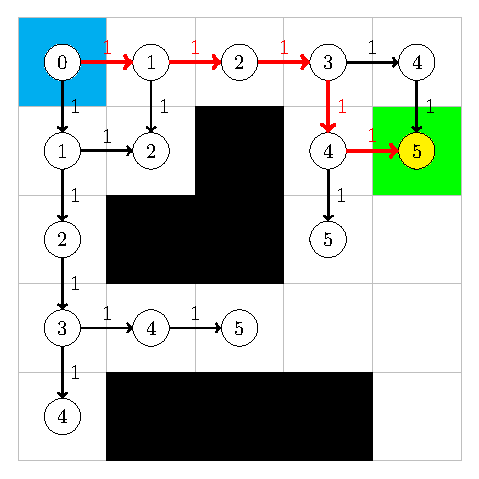
\includegraphics[width=\textwidth]{Corps_rapport/plan4.pdf}
        \caption{Résultat de l'exploration de la carte}
        \label{fig:image4}
    \end{subfigure}
    \caption{Fonctionnement de l'algorithme de Dijkstra}
    \label{fig17}
\end{figure}

\indent Face au probleme d'exploration aveugle (brute-force) dont fait face l'algorithme de Dijkstra, l'amélioration apportée par l'algorithme A* est d'ajouter un terme appelé l'heuristique dans le coût d'un noeud qui fournit une estimation du coût pour rejoindre l'objectif depuis ce noeud.\\
\indent Le coût utilisé lors de la sélection du noeud à explorer suit alors l'équation \eqref{eq2} :\\

\begin{equation} \label{eq2}
    f(n)=c(n)+h(n)
\end{equation}

où $c(n)$ est la somme des poids pour atteindre le noeud $n$ (comme dans l'algorithme de Dijkstra) et $h(n)$ est l'heuristique ajoutée pour aiguiller l'exploration vers l'objectif.\\

\indent Cette modification provoque une exploration plus rapide du graphe dès lors que l'heuristique est correctement choisie. Ce qui entrainne une reduction de la charge computationnelle dans le temps, ainsi qu'une plus faible mobilisation et consommation de ressources.\\
\indent Dans notre cas, l'heuristique est la distance à vol d'oiseau entre le noeud et l'objectif tandis que le poids entre deux noeuds est une somme entre la distance parcourue, un critère sur la similitude par rapport à la planification précédente sur les premiers mètres du chemin (afin d'éviter des oscillations) et un critère pondéré lié à la carte de coût du MNE. Le niveau de risque acceptable par le robot peut ainsi être choisi en modifiant la pondération de ce dernier coût, une faible pondération impliquant un chemin pouvant plus se rapprocher des obstacles détectés.\\
\indent La carte de coût utilisée (Figure \ref{fig18}) est similaire à une CostMap de ROS*, avec une zone critique définie autour de chaque obstacle correspondant aux zones où l'on considère que le robot va entrer en collision, une zone de danger où l'on considère que selon l'orientation le robot peut entrer en collision et un champ de potentiel décroissant avec la distance à l'obstacle.

\begin{center}
    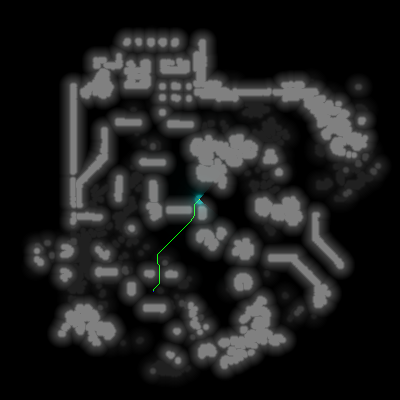
\includegraphics[width=0.4 \linewidth]{Corps_rapport/costmap.png}
    \captionof{figure}{Carte de coût utilisée par la planification globale}
    \label{fig18}
\end{center}

\indent Les zones critiques sont par définition impossibles à traverser tandis que les zones de dangers sont fortement pénalisées car il peut y avoir collision selon l'orientation du robot et sont donc souvent considérées uniquement lorsqu'il n'y a pas de solution alternative. Etant donné le manque de prise en compte de l'orientation du robot et l'absence de prise en compte de son modèle d'évolution, les chemins traversant des zones de danger pourraient ne pas être valides au sens de la traversabilité mais la brique de contrôle en aval, la planification locale, qui elle prend en compte l'orientation et l'enveloppe réelle (rectangulaire) du robot peut quand même trouver une solution à partir de ce chemin. Le surcoût computationnel qui interviendrait si l'on modifiait la carte de coûts en fonction de l'orientation du robot a encouragé à choisir ce compromis, en sachant que seuls les premiers mètres du chemin nous intéressent pour trouver une direction de déplacement privilégiée.\\
\indent Les algorithmes de Dijkstra et A* fournissent une solution optimale pour la situation donnée : carte échantillonnée et heuristique donnée pour l'A*. Il existe d'autres algorithmes de planification permettant de s'affranchir de la limitation de l'échantillonnage et permettant d'explorer l'environnement plus rapidement en générant des noeuds aléatoirement dans la carte et en essayant de les relier pour former un chemin jusqu'à l'objectif comme la Probalistic RoadMap \cite{prm1996}, le RRT \cite{rrt2000} et le RRT* \cite{rrtstar2011}. Les chemins générés ne sont plus optimaux et peuvent ne pas fournir de solution alors qu'il en existe une du fait du caractère aléatoire mais permettent de générer des chemins pouvant tenir compte de la cinématique du robot en appliquant une règle particulière lors de la génération des noeuds.

\subsubsection{Suivi de lisière}
Le suivi de lisière se compose de deux modules séquentiels : un module de détection des lisières issu de l'INRAE \cite{deremetz} et un module de suivi des lisières détectées.\\
\indent Le module de détection prend en entrée la carte de gradients seuillée pour les obstacles infranchissables fournie par le MNE, représentant une carte d'occupation 2D (carte encodant la présence d'obstacles, de manière probabiliste ou binaire), et donne en sortie au maximum deux lisières, une à gauche et une à droite. Il génère ensuite une trajectoire associée à une des deux lisières, en fonction du choix de l’utilisateur (suivre la lisière de droite ou de gauche) et l'envoie au module de suivi pour le calcul des commandes et leur envoi à la brique de supervision.\\
\indent La méthode de détection active de lisière implémentée repose sur l'adaptation de la détection de forme Snake contour et l'algorithme « Ball-Pivoting ». Cette approche permet de capturer uniquement les contours extérieurs des structures les plus proches du robot. La carte d'occupation peut avoir une certaine épaisseur pour des structures non "pleines", comme une haie clairsemée. Dans ce cas, extraire uniquement le contour extérieur permet d'éviter le traitement des points internes et de prévenir l'influence de points d'arrière-plan plus denses.\\
\indent L’algorithme de détection commence par la détection du départ de la lisière à gauche et à droite du robot. Pour cela, on translate un cercle jusqu’à ce que celui-ci intersecte un point. Ce point correspond au premier point de la lisière (Figure \ref{fig19}) :\\

\begin{center}
    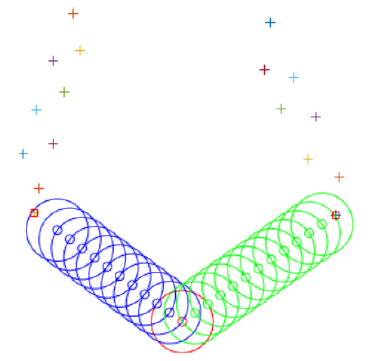
\includegraphics[width=0.3\linewidth]{Corps_rapport/lisiere1.png}
    \captionof{figure}{Détection du premier point}
    \label{fig19}
\end{center}
$\ $\
\indent Ensuite, on fait pivoter le cercle pour capturer l'ensemble des points de contour de la lisière (Figure \ref{fig20}) :\\
 \begin{center}
    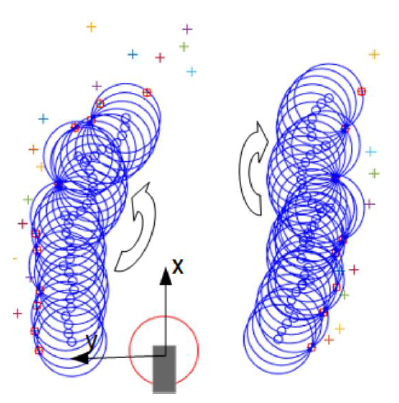
\includegraphics[width=0.3\linewidth]{Corps_rapport/lisiere2.png}
    \captionof{figure}{Détection du contour de la lisière}
    \label{fig20}
\end{center}
$\ $\
\indent Une fois les points de contour identifiés, des points intermédiaires sont ajoutés pour créer un nuage de points de chaque côté, formant une structure serpentine. Ces "serpents" représentent les bords estimés des lisières scannées (Figure \ref{fig21}) :\\
 \begin{center}
    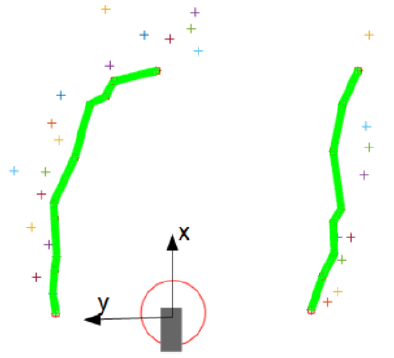
\includegraphics[width=0.3\linewidth]{Corps_rapport/lisiere3.png}
    \captionof{figure}{Création du "serpent" à partir des points de contacts du cercle et des points intermédiaires}
    \label{fig21}
\end{center}
$\ $\

\indent L’algorithme de détection de lisière est paramétrable. La taille du cercle a un grand impact sur la capacité de détection. Un cercle de petit diamètre permet d’obtenir un contour précis mais fonctionne mal avec les lisières naturelles qui possèdent de nombreuses aspérités. A l'inverse, un cercle de plus grande taille permet de passer au-dessus des aspérités et d’obtenir des lisières plus rectilignes. Les incréments de translation et de rotation du cercle sur le nuage de points permettent de maîtriser la précision du contour final. On peut également limiter la rotation du cercle sur le contour avec un angle maximal, afin d’éviter de détecter l’arrière de la lisière à la fin de cette dernière. Enfin, on limite la taille maximale du snake afin d’éviter des fausses détections et se concentrer sur la lisière en cours.\\
\indent Une fois les lisières détectées, elles sont décalées suivant leur direction normale moyenne et envoyées à l’algorithme de suivi comme trajectoires à suivre. Le module de suivi de trajectoire met en jeu un algorithme de suivi de chemin permettant une régulation latérale et longitudinale.\\
\indent La régulation latérale est réalisée par un correcteur Pure-Pursuit. Ce correcteur a pour objectif de calculer un taux de lacet à partir d'un arc de cercle reliant le centre du repère du robot à un point mobile P placé sur le chemin, en avance de phase du projeté orthogonal H du point O sur le chemin. Pour augmenter la stabilité de la régulation et réduire les oscillations à haute vitesse, le point de visée anticipée P est placé à une distance curviligne l du point H, où l est proportionnel à la vitesse de suivi.\\
\indent La régulation longitudinale est réalisée par un contrôleur qui détermine la vitesse de suivi en fonction de la vitesse consigne, de la distance à la fin du chemin et de la courbure du chemin en avance de phase. Cela permet de diminuer la vitesse à l'approche de virages ou de l'objectif.\\
\indent Cette régulation est implémentée comme une étape de minimisation d'un critère \eqref{eq3} formulé comme une somme pondérée du carré de la différence de vitesse à la vitesse de référence et de la moyenne de l'accélération centripète sur une portion du chemin à parcourir.\\
\begin{equation} \label{eq3}
    J(v)=\mu_1.(v_{max}-v)^2+\mu_2\frac{1}{n}\sum_{k=1}^n\frac{v^2}{R_{curv}(k)}
\end{equation}
$\ $\\
avec $v$ la vitesse à optimiser en $m.s^{-1}$, $v_{max}$ la vitesse de consigne en $m.s^{-1}$, $n$ le nombre de points de la portion de chemin et $R_{curv}(k)$ le rayon de courbure en $m$ du chemin au point k.\\

\indent Cette brique répondant parfaitement aux attentes du défi 2 qui ne prévoyait pas la présence d'obstacles sur le chemin, elle sera modifiée de manière à ce que le chemin de suivi de lisière généré s'adapte aux obstacles détectés par le MNE et que le robot puisse les contourner. Cette modification sera faite dans le cadre du défi 3.

\subsection{Briques de contrôle}
L'objectif des briques de contrôle est de retourner des commandes, ici de vitesses linéaires et angulaires, pour suivre un chemin donné en entrée en tenant compte de certains critères.

\subsubsection{Retour sur traces et rejeu de trajectoire}
Le retour sur traces et le rejeu de trajectoire sont assurés par la même brique, permettant d'enregistrer en temps réel la trajectoire du robot pour ensuite l'envoyer en entrée du même module de contrôle utilisé par le suivi de lisière avec un paramétrage spécifique pour fournir les commandes de déplacement à la brique de supervision.\\
\indent Pour assurer le déplacement dans un sens ou dans l'autre, il suffit d'inverser ou non les points du chemin, les consignes de vitesse et le cap du robot.







\subsubsection{Planification locale}
La planification locale se fait dans l’espace de la commande projetée en vue de dessus $(v_{2d},\dot{\alpha}_z)$, $v_{2d}$ étant la vitesse linéaire et $\dot{\alpha_z}$ la vitesse angulaire selon l'axe Z en 2D, en se servant de la carte de gradients seuillée pour les obstacles non franchissables.\\
\indent L’algorithme de planification utilisé est une adaptation de la Dynamic Window Approach (DWA) \cite{fox1997dynamic}. La méthode repose sur l'exploration de l'espace de commande afin de découvrir des combinaisons appropriées par la formulation d'un problème d'optimisation sur un horizon temporel glissant, plus étendu que l'intervalle de commande. L'avantage d'une telle approche pour la planification locale réside dans l'admissibilité cinématique des commandes tandis qu'une approche se limitant à l'espace de la tâche peut engendrer des chemins non praticables. Par exemple, l'utilisation de la planification donnée par le A* basée sur un environnement discrétisé et des champs de potentiels peut produire des inflexions abruptes dans un chemin qu'un robot non holonome ne peut suivre : le robot est incapable d'effectuer "un pas de côté" pour éviter un obstacle.\\
\indent D'autres alternatives de la DWA existent \cite{akmandor20203d, ozdemir2018follow} mais les recherches récentes tentent d'intégrer les contraintes de cinématique et la notion de risque directement dans la carte \cite{rummelhard2014probabilistic, laconte2021lambda, laconte2021novel, benrabah2023dual} ou d'utiliser l'apprentissage pour calculer les commandes optimales à exécuter \cite{hill2022online}. Cependant, ces algorithmes sont plus coûteux en temps de calcul.\\
\indent Des primitives de déplacement de type “arc” en vue de dessus (Figure \ref{fig22}) sont évaluées sur un horizon temporel de $2\ s$.  Chaque arc est paramétré par une paire de vitesses $(v_{2d},\dot{\alpha}_z)$ constantes sur la fenêtre temporelle.\\

\begin{center}
    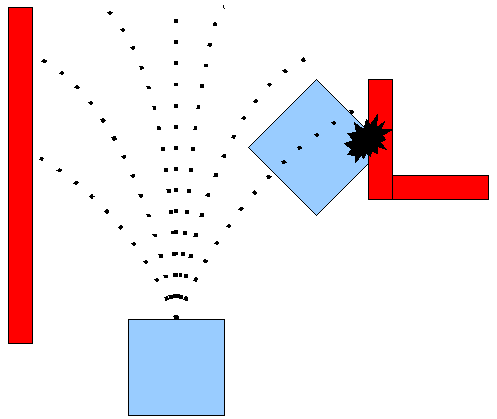
\includegraphics[width=0.3\linewidth]{Corps_rapport/DWA_illustration.png}
    \captionof{figure}{Illustration des trajectoires évaluées par la planification locale DWA}
    \label{fig22}
\end{center}


\begin{comment}
\indent Le principe de base de l'algorithme « Dynamic Window Approach » (DWA) est le suivant :\\
\begin{itemize}
\renewcommand{\labelitemi}{$\bullet$}
    \item Effectuer un échantillonnage discret dans l'espace de contrôle du robot (dx, dy, dtheta).
    \item Pour chaque vitesse échantillonnée, effectuer une simulation vers l'avant (\hyperref[fig22]{Figure 22}) à partir de l'état actuel du robot afin de prédire ce qui se passerait si cette vitesse était appliquée pendant une (courte) période.
    \item Évaluer (noter) chaque trajectoire résultant de la simulation vers l’avant, à l’aide d’un indicateur intégrant des caractéristiques telles que : la proximité des obstacles, la proximité de l’objectif, la proximité de la trajectoire globale et la vitesse. Écarter les trajectoires illégales (celles qui entrent en collision avec des obstacles).
    \item Choisir la trajectoire ayant obtenu le meilleur score et envoyer la vitesse associée à la base mobile.
    \item Répéter l’opération. \\
\end{itemize}
\end{comment}

\indent Le critère optimisé est un critère élaboré par SHERPA Engineering, fonction de l'écart par rapport à la vitesse consigne, de la direction / orientation du robot par rapport à l'objectif et de la présence d'obstacles. Il apparaît que selon la configuration d’obstacles, il n’y a aucune raison pour que ce critère soit convexe. \\
\indent Ce critère est optimisé avec une approche en force brute de type grid search: cette approche consiste à discrétiser l'espace de commande puis calculer le coût associé à chaque paire de commandes. La paire avec le plus faible coût étant la commande optimale pour la discrétisation donnée. Une fois la paire optimale trouvée, on calcule les commandes à envoyer au robot $(v,\omega_z)$ pour les adapter à la topologie du terrain dans le repère 3D.\\

\indent L'évaluation du terme de la présence des obstacles est lourd en calculs car il demande de générer l'empreinte du robot sur $2 s$ pour chaque paire de commandes. L'empreinte pour une paire de commande étant invariante, ces dernières sont générées en amont du lancement de la Brique MOBILEX* et stockées sous forme de LUT (Look-Up Tables). Lors du lancement de la brique de planification locale, elles sont chargées en mémoire vive, permettant de gagner un temps considérable pour trouver la commande optimale à appliquer. La superposition de l'empreinte et de la carte d'obstacles dans le repère du robot permet d'évaluer la présence d'obstacles sur la trajectoire générée.\\
\indent Une optimisation de cette brique à ete operée dans le cadre du defi 3. cette optimisation consiste à réduire la taille mémoire des LUT en ne stockant que les empreintes du robot à différentes orientations 








\begin{comment}

\subsubsection{Asservissement du taux de lacet}
\indent Le Barakuda est contrôlé en fournissant une consigne de vitesse identique aux roues d'un même côté, lui conférant ainsi une cinématique de type "skid steer". Avec ce type de cinématique, les roues avant et arrières dérapent nécessairement pour que le robot puisse tourner, contrairement à une cinématique à deux roues différentielles et une roue libre majoritairement employée en robotique indoor. Par conséquent, on ne peut pas faire l’hypothèse que le robot réalise vraiment le taux de rotation souhaité avec les vitesses de roue envoyées à gauche et droite en utilisant les équations d’un modèle cinématique différentiel à 2 roues sans glissement.\\\\
\indent Une solution simple et couramment employée pour résoudre ce problème consiste à asservir le taux de lacet pour que ce dernier corresponde bien aux commandes de haut niveau. Pour ce faire, on utilise les données odométriques fournie par le capteur INS pour obtenir le taux de lacet à tout instant. \\\\
\indent La correction implémentée est un simple correcteur Propotionnel Intégral avec un gain FeedForward. Le gain FeedForward joue le rôle d’un précompensateur trivial : inversion du gain $K = \lim_{\ s\ \rightarrow\ 0} H(s)$ où H est la fonction de transfert du système linéarisé. Le gain proportionnel fait l’essentiel de la régulation tandis que le gain intégral limite l’écart statique et l’effet des perturbations. Le gain feedforward augmente les performances en asservissement (précompensateur) en ramenant le système à un système à gain unitaire, tandis que le correcteur Proportionnel Intégral fait la régulation.\\\\
\indent Avec un modèle linéarisé $H(s)$ du Barakuda, il serait théoriquement possible 
d’augmenter les performances en régulation et ainsi réduire l’erreur de traînage (pour une consigne dynamique) sur le taux de lacet en remplaçant ce correcteur par un correcteur de type RST \cite{RST} que nous pourrions paramétrer pour obtenir un comportement souhaité de manière plus précise.

\end{comment}

\subsection{Autres briques}

\subsubsection{Interface avec le Barakuda}
Cette brique est responsable de la communication avec le Barakuda via des trames UDP. D’une part, elle fait remonter les informations provenant du robot au reste du système sous forme de diagnostics et, d’autre part, elle lui envoie les consignes de contrôle.

\begin{comment}
D’autre part, les consignes corrigées par le correcteur cinématique sont envoyées au robot, selon les formules habituelles \eqref{eq4} :\\

\begin{equation} \label{eq4}
    \Omega_{roues}=S\left(v_x\pm\omega_z\frac{L}{2}\right)
\end{equation}
$\ $\\
avec $\Omega_{roues}$ la vitesse de rotation des variateurs en $rpm$, $v_x$ la vitesse linéaire souhaitée en $m.s^{-1}$, $\omega_z$ la vitesse angulaire souhaitée en $rad.s^{-1}$, $L$ la voie (largeur) du véhicule en $m$ (ici, 0.95 m), et $S$ un facteur d’échelle dépendant des variateurs (ici, 1000 $rpm.s.m^{-1}$). 
\end{comment}

\subsubsection{Téléopération à la manette}
Cette simple brique lit et convertit les positions du joystick en commandes linéaires et angulaires avec un facteur d'échelle pour les envoyer directement au robot. L'ajout de la planification locale avec une configuration particulière entre cette brique et le robot permet de réaliser le mode safety first, empêchant le robot d'entrer dans des obstacles en modifiant légèrements les commandes problématiques transmises ou en arrêtant le robot.

\subsubsection{Brique de supervision}
Cette brique récupère l'ensemble des commandes fournies par les fonctions de pilotage et permet à l'opérateur de choisir laquelle est envoyée au robot via une liste déroulante dans l'IHM. Elle est également responsable d'une partie de la sécurité du robot puisqu'elle peut limiter la vitesse de ce dernier tout en gardant la même trajectoire lorsque la commande reçue provoque un dépassement du seuil de l'accélération centrifuge autorisé ou encore provoquer l'arrêt et le serrage des freins lors d'un dysfonctionnement grave retourné par une brique. La commande vérifiée ou limitée est ensuite envoyée au robot.

\subsubsection{Retour visuel annoté pour l'opérateur}
Cette brique utilise le retour image de la caméra frontale du système de perception pour y superposer différentes informations, éventuellement agrégées à partir des autres modules. \\
\indent Afin de respecter les exigences du challenge Mobilex*, les 
informations suivantes sont superposées au flux image : \\
\begin{itemize}
\renewcommand{\labelitemi}{$\bullet$}
    \item Affichage type “Viseur Tête Haute“ avec les angles de roulis, tangage, et lacet.
    \item Tracé des chemins de navigation trouvés par la planification globale en 3D.
    \item Tracé du chemin local à court terme (2 $s$), étant donné la commande actuelle.
    \item Représentation des obstacles avec des régions colorées en fonction de la distance.
    \item Representation colorée des flaques d'eau et végétation traversable 
    \item Représentation des waypoints en 3D dans l’image.
    \item Compas\\
\end{itemize}

\indent La projection dans l’image des informations définies dans le repère monde a été réalisée à l'aide de la calibration intrinsèque de la caméra ainsi que de la calibration extrinsèque caméra/LIDAR* réalisée auparavant et du système de transformations tf de ROS* permettant de définir une matrice de transformation homogène 4x4 pour projeter les éléments du repère monde vers le repère image. Cette transformation est utilisée pour la représentation des obstacles, des waypoints, des flaques d'eau, des végétations traversables et des chemins afin d'obtenir le retour annoté (Figure \ref{fig23}).

\subsubsection{IHM}
Enfin, la brique IHM fournit une interface graphique (Figure \ref{fig23}) sur le PC débarqué à l'aide du framework ROS* RQT. Elle permet au téléopérateur d'accéder au retour visuel annoté, d'envoyer des ordres de mission tout en ajustant les paramètres à sa guise, et d'enregistrer des trajectoires pour les modes « rejeu » et « retour sur traces ». Elle offre également la possibilité de saisir des coordonnées de points à atteindre, de consulter un ensemble de données et de diagnostics pour le débogage, ainsi que de définir et charger des paramètres pour les modes dégradés (hautes herbes, brouillard, etc.).

\begin{center}
    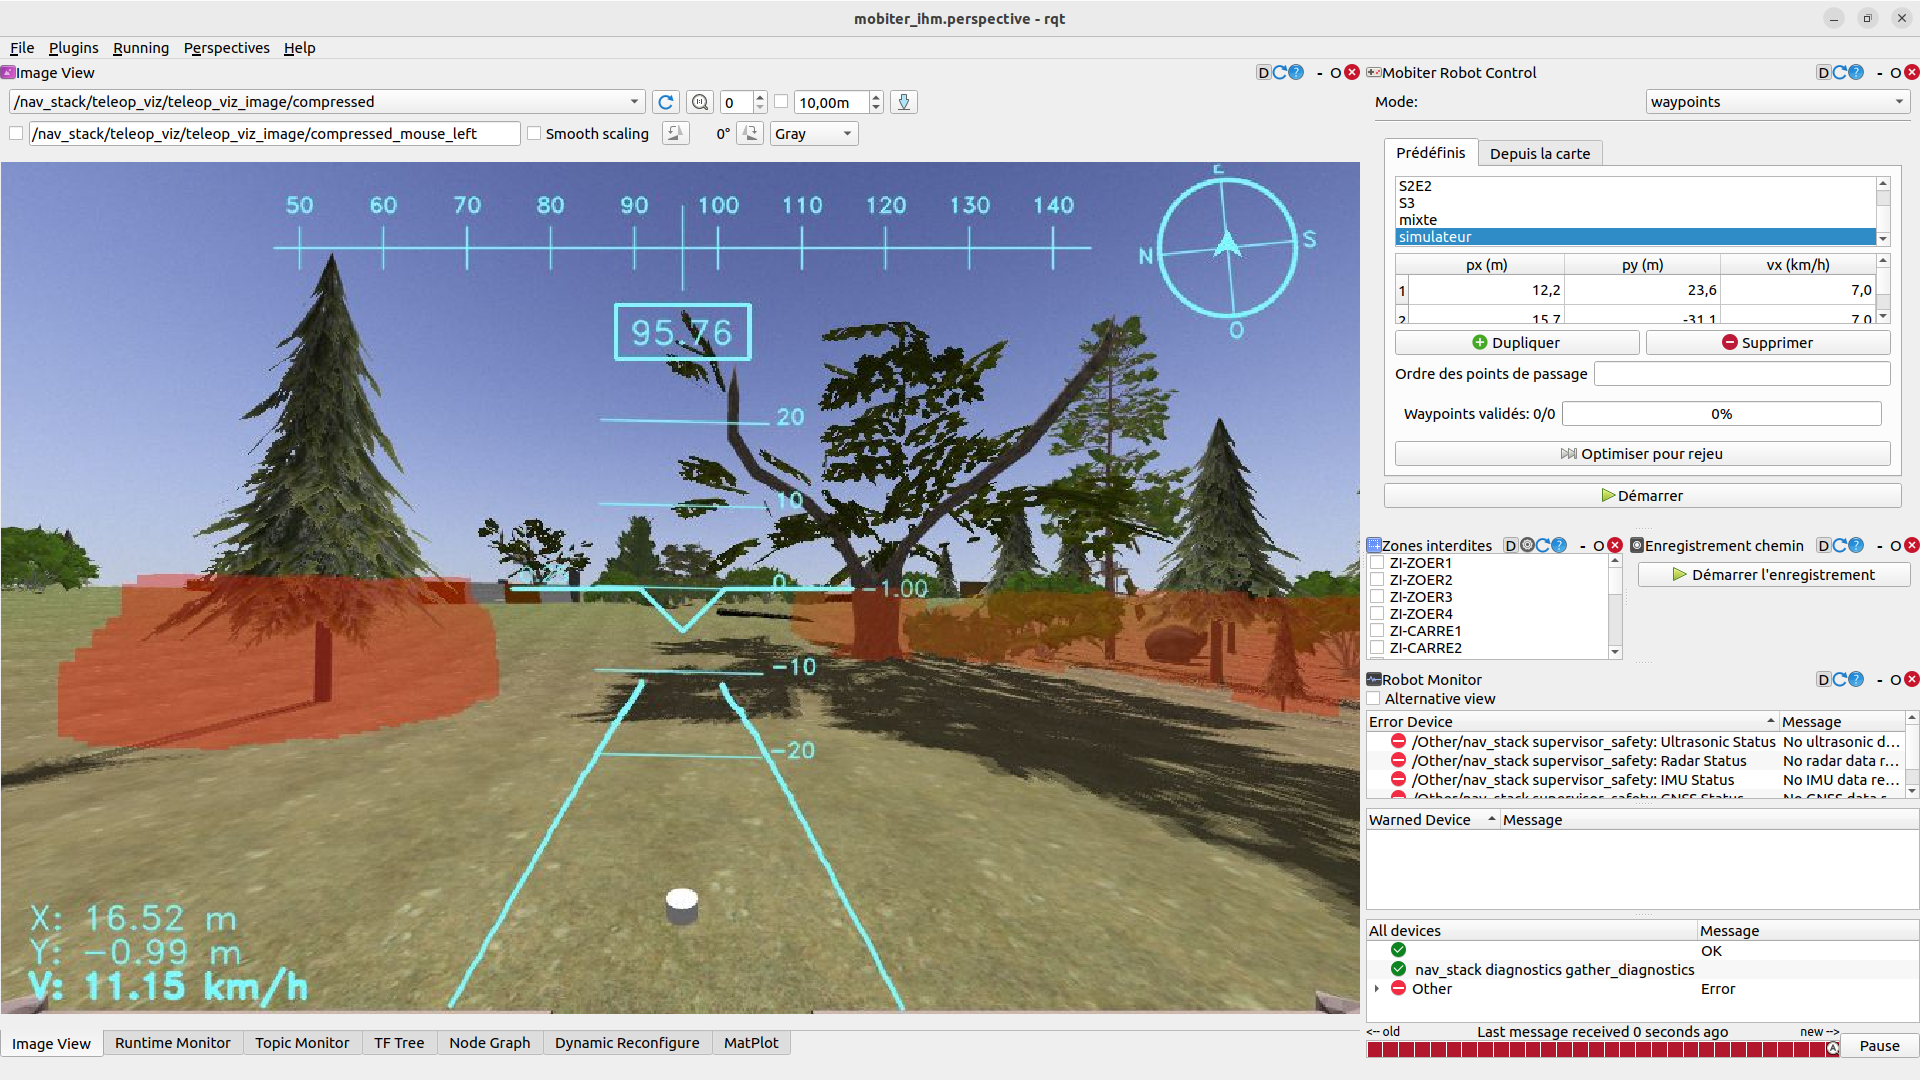
\includegraphics[width=0.9\linewidth]{Corps_rapport/rqt.png}
    \captionof{figure}{Interface RQT}
    \label{fig23}
\end{center}

\indent En parallèle de l'interface RQT, une visualisation RVIZ (Figure \ref{fig24}) peut être lancée. Elle permet d'afficher les différentes cartes générées par la brique MNE, d'observer les chemins planifiés et d'indiquer un point cible directement sur la carte. Une légende y est associée afin d'en faciliter la compréhension.

\begin{center}
    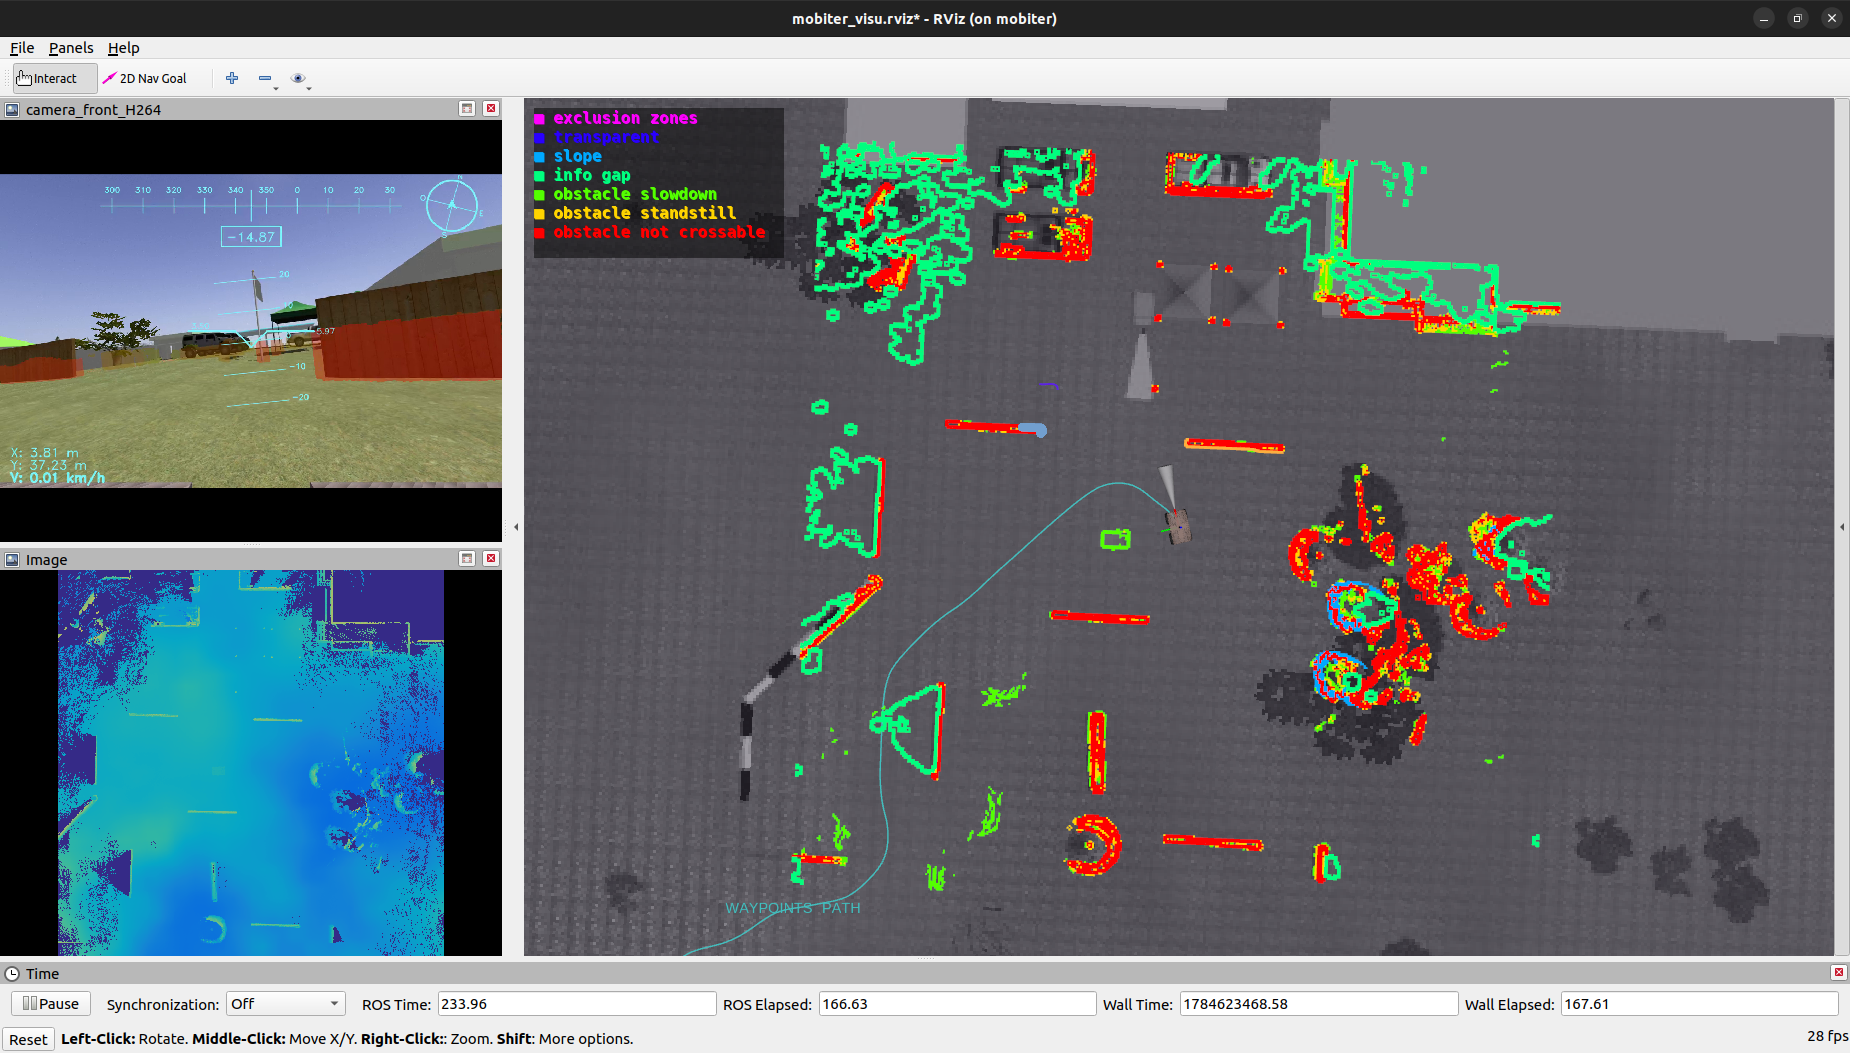
\includegraphics[width=0.9\linewidth]{Corps_rapport/rviz.png}
    \captionof{figure}{Visualisation RVIZ}
    \label{fig24}
\end{center}

\newpage
\section{Le stage}
\subsection{Les missions}
J'ai été recruté comme stagiaire chez SHERPA Engineering afin d'apporter une aide à l'intégration et aux tests terrain pour compte du défi 3 du Challenge MOBILEX*.\\\\
\indent Ma mission principale consiste à participer aux tests des différentes briques logicielles développées sur le robot. Les tests se font d'abord en simulation, puis, lorsque les résultats sont concluants, sur le terrain. Lors des tests terrains, il est nécessaire de prévoir une série de tests pertinents pour mettre à l'épreuve les briques sous test et de communiquer avec l'équipe de l'INRAE pour programmer une date et prévoir la disponibilité du matériel à utiliser pour les tests. Une fois les tests réalisés, un compte-rendu est fait à l'équipe de développement.\\\\
\indent En cas de problèmes lors des tests, il est impératif de noter les circonstances dans lesquelles ils sont apparus, trouver des scénarios reproduisant ces derniers, réaliser des diagnostics, isoler la cause et, dans la mesure du possible, proposer une solution de résolution.\\\\
\indent En dehors des sessions de tests planifiées, mes missions se sont articulées autour de deux axes principaux : \\

\begin{itemize}
\renewcommand{\labelitemi}{$\bullet$}
    \item \textbf{L'automatisation du post-traitement} : J'ai développé un générateur automatique de rapports d'essais. Cet outil synthétise les données d'exécution afin de fournir une analyse visuelle et rapide du déroulement des tests.
    \item \textbf{La standardisation des procédures} : J'ai mis sur pied un protocole et un plan de test rigoureux. Ce cadre méthodologique vise d'une part à évaluer la conformité du système vis-à-vis des exigences fonctionnelles spécifiées par la DGA pour le Défi 3, et d'autre part à garantir la répétabilité des scénarios d'essai, indépendamment de l'ingénieur chargé de l'exécution.\\
\end{itemize}
    
\indent Enfin, j'ai travaillé sur l'amélioration de la fonctionnalité de suivi de lisière en y intégrant une prise en compte des obstacles sur le chemin.


\subsection{Présentation des travaux réalisés}

\subsubsection{Prise en main du projet}
Lors de mon arrivée à SHERPA Engineering, il a été indispensable pour moi de prendre en main un projet débuté depuis plus de deux ans.\\\\
\indent Mon premier objectif a consisté à cloner le dépôt Git de l'ensemble du projet Mobiter sur notre poste de travail. Ce dernier fonctionne sous Ubuntu 22.04 et intègre Distrobox, un outil de conteneurisation permettant d'exécuter une surcouche logicielle sous un autre système d'exploitation — en l'occurrence Ubuntu 20.04. Cette configuration est indispensable pour utiliser ROS Noetic. En effet, l'intégralité de la brique logicielle MOBILEX a été développée sous cette version de ROS, qui s'avère incompatible avec la distribution native Ubuntu 22.04. \\\\
\indent Une fois le simulateur fonctionnel, j'ai alors pu me familiariser avec l'utilisation de l'IHM et les différents modes de conduite disponibles. Puis afin de pouvoir proposer des tests pertinents et comprendre l'architecture logicielle de la brique MOBILEX*, aussi bien d'un point de vue théorique que technique, il m'a fallut consulter l'ensemble des codes.

\subsubsection{Migration et évaluation du SLAM (Simultaneous Localization and Mapping)}

La pile logicielle (stack) MOBITER nécessite une estimation de pose précise et continue. Si la disponibilité permanente du GNSS RTK lors du défi 1 garantissait ces conditions, l'introduction de coupures GNSS temporaires lors du défi 2 ($< 2\text{ min}$) a imposé l'intégration d'une solution alternative. Un algorithme de SLAM LiDAR (\textbf{Kitware}), couplé à une extrapolation IMU pour augmenter la fréquence d'échantillonnage, a été déployé conjointement avec un module d'arbitrage chargé d'assurer la transition entre les sources de localisation. Bien que fonctionnelle pour le défi 2, cette architecture a révélé deux limitations majeures : \\

\begin{itemize}
    \item \textbf{Une dérive spatiale critique} : Fortement dépendante de la structure géométrique de l'environnement, la dérive intrinsèque du SLAM kitware engendrait des discontinuités de pose (sauts de localisation) trop importantes lors de la réacquisition du signal GNSS. Pour prévenir tout comportement instable, le module d'arbitrage interdisait le basculement si l'écart mesuré dépassait un seuil critique, contraignant le robot à poursuivre sa navigation en mode SLAM dégradé jusqu'à la fin de la mission.
    \item \textbf{Une charge computationnelle élevée} : Le SLAM de Kitware constituait le processus le plus budgétivore en ressources calcul de la stack, risquant d'induire des verrous de performance avec l'ajout de nouvelles fonctionnalités.\\
\end{itemize}

Face à l'allongement prévisible des masquages GNSS lors du défi 3, le SLAM LiDAR de Kitware a été remplacé par l'approche \textbf{DLIO*} (Direct LiDAR-Inertial Odometry), caractérisée par une dérive significativement plus faible. Parallèlement, un gestionnaire de discontinuité de localisation a été ajouté pour faire face à la discontinuité de pose lors des transitions SLAM$\rightarrow$GNSS, garantissant le réengagement du GNSS RTK quelle que soit la dérive cumulée tout en maintenant le suivi du scénario.\\

\begin{comment}
Au début de mon stage, l'équipe Mobiter avait engagé des travaux de refonte du module de SLAM (Simultaneous Localization and Mapping). Lors des défis précédents, la solution logicielle reposait exclusivement sur le Kitware SLAM, une approche purement LiDAR. Celle-ci présentait de graves limites dans les environnements très dégagés (comme les grands espaces extérieurs), où la rareté des caractéristiques géométriques et des retours LiDAR nuisait à la qualité de la localisation. De plus, ce composant représentait l'une des charges computationnelles les plus lourdes de la pile logicielle du projet. Afin de pallier ces défauts, le SLAM DLIO (Direct LiDAR-Inertial Odometry), combinant les données LiDAR et une centrale inertielle (IMU), a été choisi comme une alternative plus robuste pour la navigation en milieux ouverts.\\\\ 
\end{comment}

\indent C’est dans ce contexte du défi 3 que j'ai participé à l'évaluation et aux tests du SLAM DLIO en simulation et sur terrain au sein de la brique MOBILEX*. Une fois son intégration logicielle finalisée, nous avons mené une campagne de tests afin de valider son bon fonctionnement et de quantifier ses performances (en matière de dérive et de charge CPU) par rapport au Kitware SLAM et à la vérité terrain.


\paragraph{Fonctionnement du Kitware SLAM}

Le \textbf{Kitware SLAM} repose sur l'algorithme LOAM* (\textit{LiDAR Odometry And Mapping in Real-time}) \cite{LOAM}, qui se décompose en trois étapes principales :

\subparagraph{a. Le prétraitement et l'extraction des caractéristiques géométriques du nuage de points LiDAR}:

La première étape consiste à prétraiter le nuage de points LiDAR afin d'atténuer les distorsions subies lors du mouvement du véhicule pendant l'acquisition, puis d'extraire les éléments géométriques nécessaires au recalage. Contrairement aux approches traitant l'intégralité des points du scan, LOAM sélectionne uniquement les points présentant une information géométrique forte. Cette sélection réduit la charge computationnelle tout en préservant les contraintes physiques indispensables à l'estimation de pose. Deux types de caractéristiques sont principalement extraits :\\

\begin{itemize}
    \item \textbf{Les points d'arêtes (\textit{edge features}) :} ils correspondent aux zones présentant une forte variation de courbure (angles de bâtiments, contours d'obstacles).
    \item \textbf{Les points plans (\textit{surface features}) :} ils identifient les zones de faible variation de courbure, représentatives de surfaces régulières (sol, murs, façades).\\
\end{itemize}

Ces caractéristiques sont ensuite exploitées lors des phases de recalage afin de calculer la transformation rigide entre deux acquisitions successives.

\subparagraph{b. L'estimation de l'odométrie LiDAR}:

La deuxième étape vise à évaluer le déplacement relatif du robot entre deux scans consécutifs. Pour cela, LOAM réalise un recalage \textbf{scan-to-scan} entre les caractéristiques extraites de l'acquisition courante et celles de la précédente. L'estimation de la transformation spatiale est obtenue par la minimisation de deux métriques d'erreur :\\
 
\begin{itemize}
    \item Une distance point-droite pour les caractéristiques d'arêtes.
    \item Une distance point-plan pour les caractéristiques de surface.\\
\end{itemize}  

L'optimisation sous ces contraintes fournit la transformation à une fréquence supérieure à celle de la cartographie. Néanmoins, ce traitement reste sujet à la dérive par accumulation des erreurs de recalage.

\subparagraph{c. La construction de la carte et l'optimisation spatiale}:

La troisième étape reconstruit progressivement la carte globale de l'environnement tout en corrigeant la dérive accumulée par l'odométrie. À l'inverse de l'étape précédente, le recalage s'effectue cette fois entre le scan courant et la carte locale (\textbf{scan-to-map}). Les caractéristiques du nouveau nuage de points sont alignées avec la carte préexistante afin d'affiner l'estimation de pose, garantissant ainsi la cohérence spatiale à long terme.\\

Bien que la documentation détaillée du \textbf{Kitware SLAM} soit restreinte, cet algorithme intègre un système d'optimisation par graphe de poses \cite{kitware_slam}, capable de réajuster l'ensemble de la carte lors d'une fermeture de boucle (\textbf{loop closure}). Il propose également une extraction enrichie de caractéristiques, incluant la détection de ruptures d'intensité lumineuse ou d'amas de points (\textbf{blobs}).
De plus, le module offre la possibilité d'injecter des données exogènes issues d'autres capteurs (IMU, GNSS, INS, odométrie des roues, caméras RGB pour balises visuelles). Toutefois, les essais expérimentaux menés n'ont pas révélé de gain de performance significatif lors de l'intégration directe de l'IMU au sein du SLAM. Cela a justifié le choix de conserver (dans le cadre du défi 2) une version exclusivement LiDAR pour le SLAM et de coupler l'IMU de manière externe afin d'élever la fréquence de la localisation. Enfin, certaines fonctionnalités avancées ont dû être restreintes afin d'assurer le respect des contraintes temps réel de la pile logicielle (\textbf{stack}).


\paragraph{Fonctionnement du DLIO* SLAM}

DLIO* (Direct LiDAR-Inertial Odometry) \cite{dlio_slam} est un algorithme d'odométrie LiDAR-inertielle sobre en calcul et conçu pour maintenir une localisation précise et construire une carte 3D dense même lors de mouvements agressifs ou dans des environnements peu structurés. Contrairement aux approches fondées sur l'extraction de primitives géométriques (LOAM, Kitware SLAM) et le recalage intermédiaire \textbf{scan-to-scan}, DLIO adopte une approche directe opérant directement sur le nuage de points dense. Il réalise un recalage direct \textbf{scan-to-map} grace aux garanties de convergence formelles de son observateur d'état. Son traitement repose sur quatre étapes clés :

\subparagraph{a. Prétraitement et conditionnement des données denses}:

La première étape consiste à réaliser un alignement spatio-temporel des données LiDAR ($10\text{--}20\text{ Hz}$) et IMU ($100\text{--}500\text{ Hz}$) dans le repère du robot sans sous-échantillonnage agressif (par grille de voxel) ni extraction de primitives (arêtes, plans, etc.). Sur le nuage de points dense est appliqué un simple filtrage spatial de proximité destiné à éliminer les points appartenant à la structure propre du robot. L'algorithme offre aussi la possibilité d’ajouter un léger sous-échantillonnage (0.05 à 0.1m) pour les LiDARs très denses.
    
\subparagraph{b. Correction de mouvement}:

Pendant la durée du balayage LiDAR, les mouvements du robot induisent des distorsions spatiales importantes. Pour éliminer ces déformations sans recourir aux simplifications classiques (vitesse constante) ni au coût de calcul élevé d’autres méthodes d’interpolation, DLIO introduit une approche séquentielle de type \textbf{coarse-to-fine} \cite{coarse_to_fine} décrite comme suit :\\

\begin{itemize}
    \item \textbf{Coarse step} : Les mesures IMU comprises entre deux scans LiDAR successifs sont intégrées numériquement sous l’hypothèse d’un modèle de mouvement d’ordre supérieur à secousse linéaire et accélération angulaire constantes. Cela permet d’obtenir une estimation de l’état du robot à chaque nouvelle valeur IMU.
    \item \textbf{Fine step} : Pour chaque point du nuage acquis à l’instant relatif $t_n$, DLIO se sert des deux états estimés par l’IMU encadrant $t_n$ pour résoudre un jeu d’équations analytiques sous forme close paramétré uniquement par l’horodatage $t_n$. Ce calcul exact et parallélisable corrige la distorsion (\textbf{deskewing}) et projette le nuage dans le repère monde $\mathcal{W}$, générant une estimation de l'état \textit{a priori} $\hat{\mathbf{T}}_{\text{prior}}^{\mathcal{W}}$ pour le recalage géométrique.\\
\end{itemize}
    
\subparagraph{c. Recalage géométrique (GICP* : Generalized Iterative Closest Point)}:

Grâce à la précision de l'estimation initiale, DLIO s'affranchit du recalage scan-to-scan et effectue directement un alignement scan-to-map. Le nuage corrigé $\hat{\mathcal{P}}_k^{\mathcal{W}}$ est aligné sur une sous-carte locale $\hat{\mathcal{S}}_k^{\mathcal{W}}$ constituée d'images-clés (keyframes). Cet alignement s'appuie sur l'algorithme GICP \cite{gicp}, qui modélise la surface locale par des matrices de covariance et minimise la distance de Mahalanobis (correspondance plan-à-plan). L'optimisation produit la transformation $\Delta \hat{\mathbf{T}}_k$, affinant ainsi la pose globale $\hat{\mathbf{T}}_k^{\mathcal{W}}$.

\subparagraph{d. Fusion et mise à jour d'état}: 

Pour fusionner les données LiDAR et IMU, DLIO intègre un observateur géométrique non linéaire hiérarchique. Il combine la pose affinée par le GICP aux mesures IMU haute fréquence afin d'estimer l'état complet du système :

\begin{equation}
    \hat{\mathbf{x}}_k = \begin{bmatrix} \mathbf{p}^{\mathcal{W}} & \mathbf{q}^{\mathcal{W}} & \mathbf{v}^{\mathcal{W}} & \mathbf{b}_a & \mathbf{b}_\omega \end{bmatrix}^\top
\end{equation}
représentant respectivement la position, l'orientation, la vitesse et les biais de l'IMU.\\
\indent Fondé sur la théorie de la contraction, cet observateur garantit une convergence globale théorique. Les états estimés sont réinjectés dans les intégrations IMU ultérieures, fermant ainsi la boucle d'estimation.


\paragraph{Comparaison expérimentale DLIO vs Kitware SLAM}

Afin de comparer la qualité de la localisation des 2 SLAM, nous avons mené une série de tests expérimentaux sur différents terrains. Sur une trajectoire de 320 mètres réalisée dans un environnement naturel relativement riche en obstacles (\hyperref[fig27]{Figure 27}), nous avons obtenu les parcours présenté en annexe \hyperref[annexe5]{[INRAE]} et les courbes suivantes (\hyperref[fig28]{Figure 28} et \hyperref[fig29]{Figure 29}) représentant les positions et orientations estimées par chaque SLAM par rapport à la vérité terrain donnée par le GNSS RTK.\\

\begin{center}
    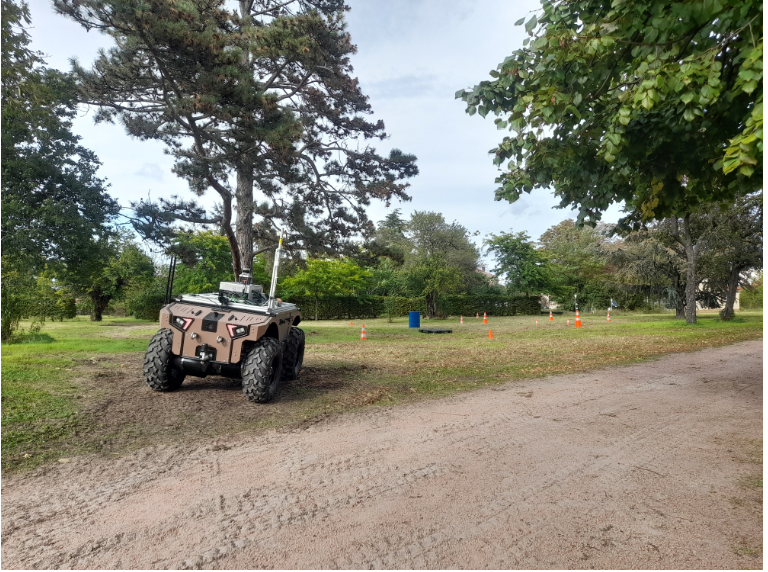
\includegraphics[width=0.5\linewidth]{Corps_rapport/inrae.png}
    \captionof{figure}{Terrain d’essais de l’INRAE Aubière}
    \label{fig27}
\end{center}

\begin{figure}[h]
    \centering
    \begin{subfigure}[b]{0.48\textwidth}
        \centering
        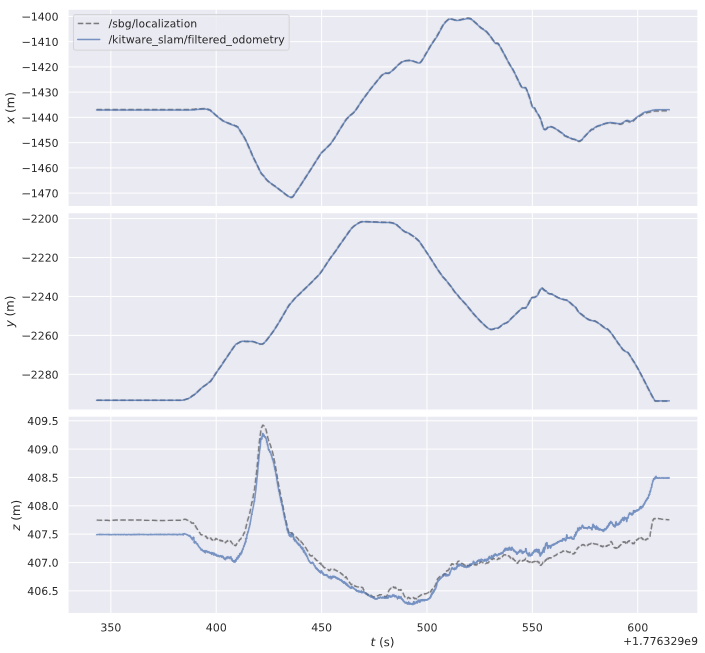
\includegraphics[width=\textwidth]{Corps_rapport/kitware_position_inrae.png}
        \caption{position évaluée par kitware}
        \label{fig:image1}
    \end{subfigure}
    \hfill
    \begin{subfigure}[b]{0.48\textwidth}
        \centering
        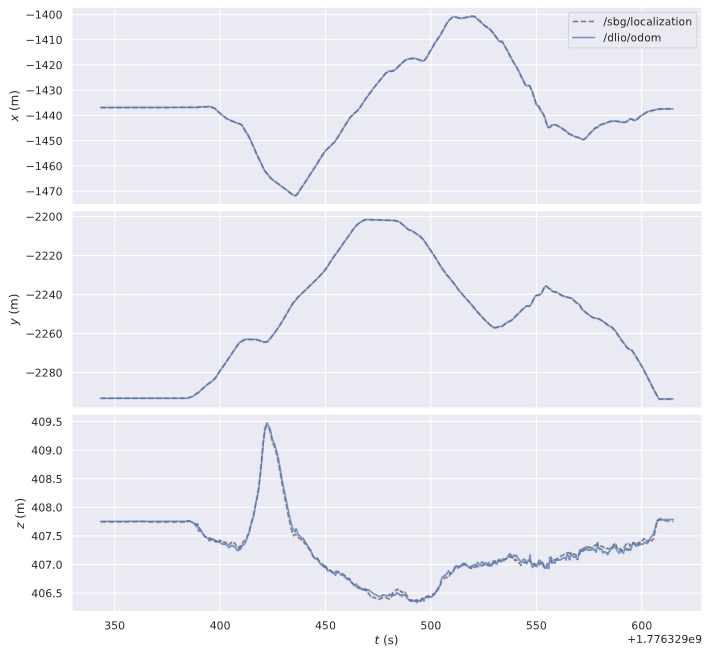
\includegraphics[width=\textwidth]{Corps_rapport/dlio_position_inrae.png}
        \caption{position évaluée par DLIO}
        \label{fig:image2}
    \end{subfigure}    
    \caption{Comparaison des positions Kitware vs DLIO vs vérité terrain}
    \label{fig28}
\end{figure}

\begin{figure}[h]
    \centering
    \begin{subfigure}[b]{0.48\textwidth}
        \centering
        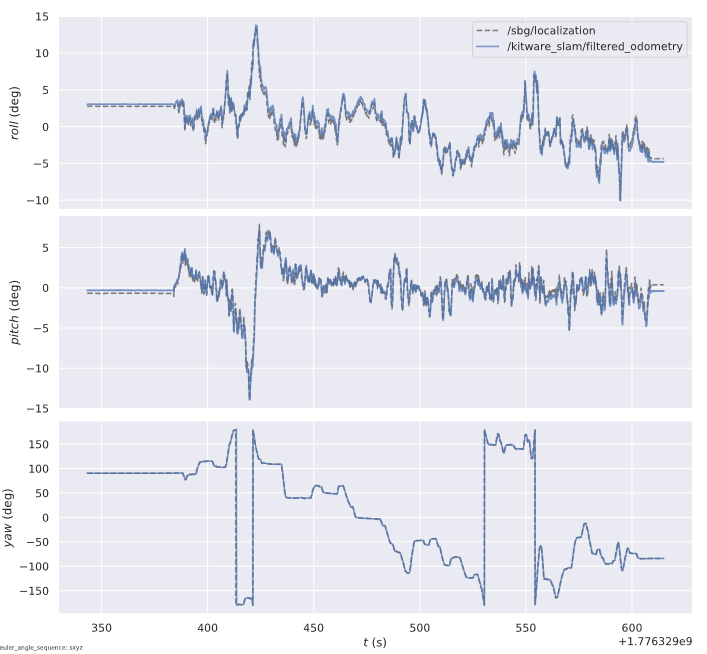
\includegraphics[width=\textwidth]{Corps_rapport/kitware_RPY_inrae.png}
        \caption{orientation évaluée par kitware}
        \label{fig:image1}
    \end{subfigure}
    \hfill
    \begin{subfigure}[b]{0.48\textwidth}
        \centering
        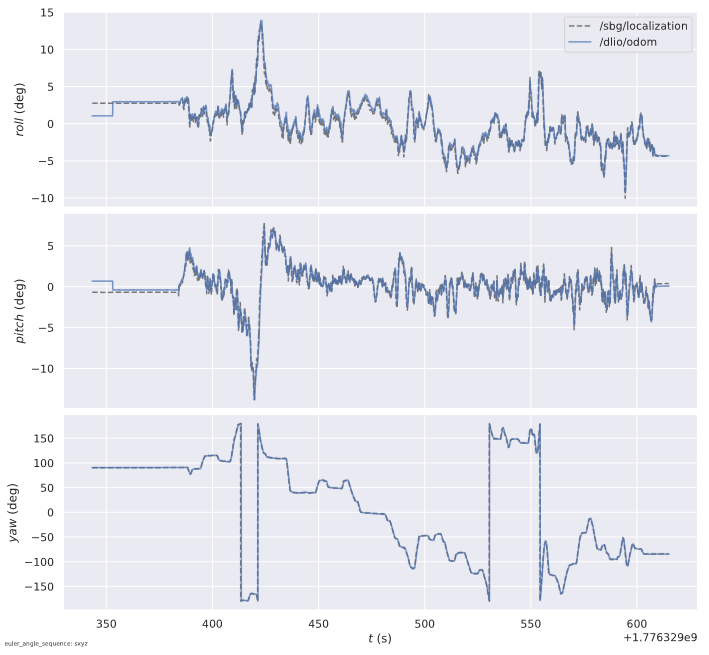
\includegraphics[width=\textwidth]{Corps_rapport/dlio_RPY_inrae.png}
        \caption{orientation évaluée par DLIO}
        \label{fig:image2}
    \end{subfigure}    
    \caption{Comparaison des orientations Kitware vs DLIO vs vérité terrain}
    \label{fig29}
\end{figure}

Au regard des courbes précedentes, on peut constater que les 2 SLAM offrent en environnement structuré des trajectoires alignées avec la vérité terrain. Cependant, le SLAM DLIO présente des erreurs de pose bien plus faible que le SLAM Kitware comme le témoigne la figure (\hyperref[fig30]{Figure 30}) ci-dessous.

\begin{center}
    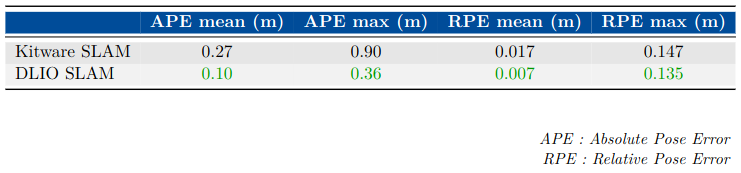
\includegraphics[width=1.0\linewidth]{Corps_rapport/Kitware_vs_dlio_metrics.png}
    \captionof{figure}{Comparaison des erreurs de pose sur le terrain d’essais de l’INRAE Aubière}
    \label{fig30}
\end{center}

Puis sur une plus longue trajectoire de près de 1 km réalisée dans un environnement naturel fortement dégagé (\hyperref[fig31]{Figure 31}), nous avons obtenu les parcours présenté en \hyperref[fig32]{Figure 32} représentant les poses estimées par chaque SLAM par rapport à la vérité terrain donnée par le GNSS RTK.\\

\begin{center}
    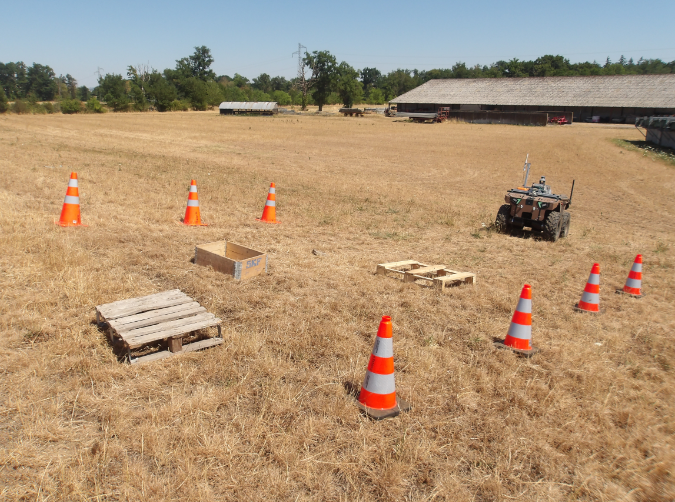
\includegraphics[width=0.5\linewidth]{Corps_rapport/montoldre.png}
    \captionof{figure}{Terrain d’essais de Montoldre}
    \label{fig31}
\end{center}

\begin{center}
    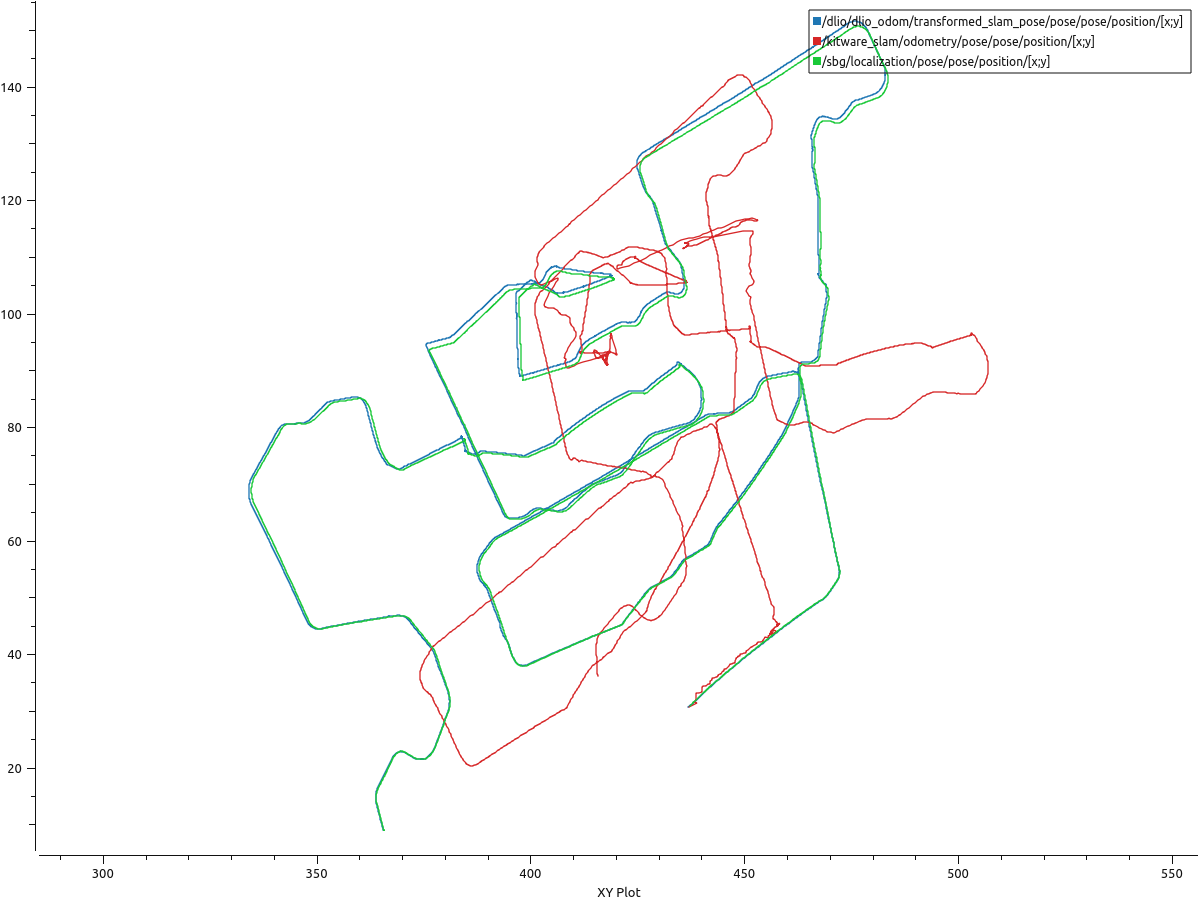
\includegraphics[width=0.8\linewidth]{Corps_rapport/dlio_vs_kitware_vs_Sbg_montoldre.png}
    \captionof{figure}{Comparaison des trajectoires DLIO vs Kitware vs vérité terrain en zone dégagée}
    \label{fig32}
\end{center}

Au regard de la figure précedente, on constate que le SLAM DLIO, grâce à son couplage inertiel-LiDAR, garantit une très bonne localisation, même en milieu dégagé. Ce n'est pas le cas du SLAM Kitware, qui montre des limites évidentes dans ces conditions. De plus, comme le montre l'annexe \hyperref[annexe6]{[montoldre]}, le SLAM DLIO présente une erreur de position maximale d'environ 1,5 mètre, tandis que celle du SLAM Kitware atteint environ 80 mètres d'erreur maximale sur ce parcours de 1 km. Enfin, on observe une réduction d’environ 50\% d’utilisation de RAM et de charge CPU avec le SLAM DLIO par rapport à notre version allégée de Kitware. Ces résultats confortent notre choix de changer de SLAM dans le cadre du défi 3.\\


\paragraph{Modifications apportées à DLIO SLAM}

Pour atteindre les performances illustrées précédemment, des modifications ont été apportées dans le code de base de DLIO. Initialement, DLIO donnait une dérive globale certes plus faible que le Kitware SLAM mais très bruité, rendant son exploitation dans la stack impossible sans dégrader la carte (\hyperref[fig33]{Figure 33}).

\begin{center}
    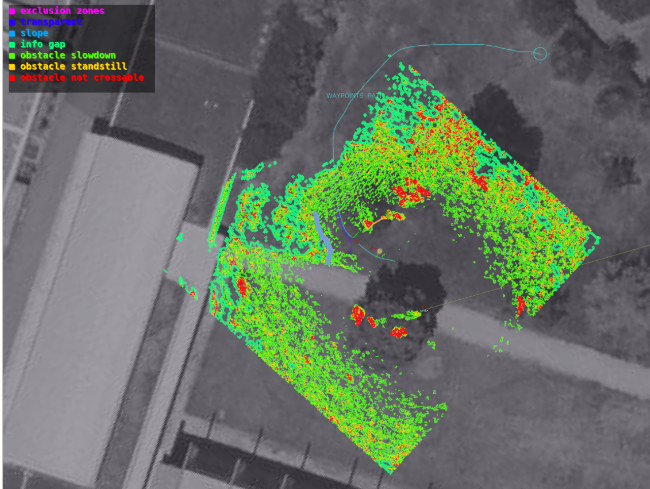
\includegraphics[width=0.5\linewidth]{Corps_rapport/map_dlio_bruit.png}
    \captionof{figure}{Carte construite avec la version originale de DLIO SLAM}
    \label{fig33}
\end{center}

Après avoir tenté d'atténuer ce bruit en ajustant les paramètres de l'observateur géométrique sans résultat concluant, une incohérence conceptuelle a été identifiée au sein du code du SLAM : \textbf{les fusions entre les observations LiDAR et IMU n'étaient pas cohérentes temporellement}.\\

Considérons $t_{\text{scan}}$ le timestamp du dernier scan LiDAR, $t_{\text{gicp}}$ le temps de calcul nécessaire au recalage GICP du scan courant sur la carte locale, et $t_{\text{now}}$ le timestamp de l'état courant (associé à la dernière fusion IMU). Dans l'implémentation originale de DLIO, la durée $t_{\text{gicp}}$ était négligée. Le résultat du recalage GICP (correspondant à la pose à $t_{\text{scan}}$) était ainsi fusionné avec un état ayant déjà évolué durant $t_{\text{gicp}}$ pour atteindre $t_{\text{now}} \approx t_{\text{scan}} + t_{\text{gicp}}$. En raison de ce décalage temporel, l'observateur géométrique calculait un écart artificiellement élevé qu'il tentait de corriger, ce qui tirait l'état du robot vers une pose passée et perturbait l'estimation des vitesses (\textit{twists}) ainsi que des biais de l'IMU.\\

Pour résoudre ce problème, un tampon (\textit{buffer}) des états fusionnés par l'observateur a été implémenté et son fonctionnement a été repensé :
\begin{itemize}
    \item \textbf{Interpolation temporelle :} Le \textit{buffer} permet d'interpoler l'état exact à l'instant $t_{\text{scan}}$ afin d'y fusionner l'observation LiDAR.
    \item \textbf{Rétropropagation :} Comme l'état continue d'évoluer pendant la phase de recalage, les mesures IMU acquises entre $t_{\text{scan}}$ et $t_{\text{now}}$ sont rejouées (rétropropagées) à partir de l'état à $t_{\text{scan}}$ corrigé par le GICP, remplaçant ainsi l'état \textit{a priori} à $t_{\text{now}}$.\\
\end{itemize}

Cette correction a permis d'accorder un poids supérieur au recalage GICP dans l'observateur, autorisant des corrections plus franches tout en réduisant la dérive globale.\\

Enfin, une dérive anormale observée en sortie de l'observateur par rapport aux résultats bruts du GICP a été résolue en substituant l'IMU intégrée du LiDAR Ouster ($100\text{ Hz}$), particulièrement bruitée, par l'IMU de la Xsens ($100\text{ Hz}$) moin bruitée. Voire annexe \hyperref[annexe7]{[pose\_gicp]} pour plus de détails. Ces modifications intégrées ont permis d'obtenir une carte de meilleure qualité et une dérive globale plus faible, comme le montre la figure ci-dessous (\hyperref[fig34]{Figure 34}).

\begin{center}
    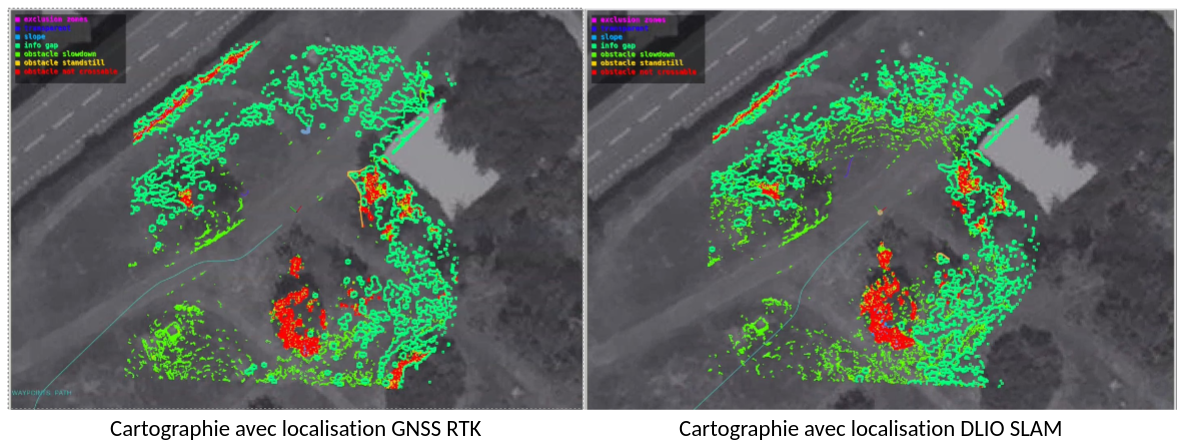
\includegraphics[width=1\linewidth]{Corps_rapport/Comparaison_map_DLIO_vs_GNSS.png}
    \captionof{figure}{Comparaison de cartographie en GNSS RTK VS en DLIO}
    \label{fig34}
\end{center}

\indent Comme le montre la figure ci-dessus, la carte générée par le SLAM DLIO est de bonne qualité et garantit une navigation fiable lorsqu'on la compare à la vérité terrain fournie avec le GNSS RTK. L'étape suivante a consisté à évaluer la dérive du SLAM DLIO par rapport à la vérité terrain en fonction de la distance parcourue.

\begin{comment}
Nous avons par la suite évalué les performances du SLAM DLIO en comparant sa trajectoire à la vérité terrain ainsi qu'à celle générée par le SLAM Kitware. C'est dans cette optique que des essais ont été menés sur les sites de l'INRAE d'Aubière et de Montoldre. La méthodologie a consisté, dans un premier temps, à enregistrer un fichier de données (rosbag) lors d'un déplacement en téléopération avec le SLAM DLIO actif, tout en enregistrant la position de référence renvoyée par la centrale de navigation SBG. Dans un second temps, ce bag a été rejoué hors ligne afin d'exécuter le SLAM Kitware et de générer un fichier unique centralisant les trois sources de localisation (GNSS RTK, DLIO et Kitware). Enfin, l'utilisation des outils de la bibliothèque EVO nous a permis de comparer et d'évaluer précisément les performances des deux algorithmes de SLAM par rapport à la vérité terrain (\hyperref[fig27]{Figure 27} et \hyperref[fig28]{Figure 28}).\\
\end{comment}


\subsubsection{Évaluation de la dérive du SLAM DLIO par rapport à la vérité terrain}

La bibliothèque python EVO, très employée pour l'évaluation de techniques de SLAM, utilise l'algorithme de Kabsch-Umeyama \cite{Kabsch} pour aligner les trajectoires avant comparaison et évaluation. Cet algorithme permet de trouver la meilleure transformation rigide (rotation et translation) qui minimise l'écart quadratique moyen (RMSD) entre deux ensembles de points appariés. Il est utile pour l'alignement d'ensembles de points en infographie, ainsi qu'en chimio-informatique et en bio-informatique pour comparer des structures moléculaires et protéiques. \\\\
\indent Cette étape de transformation est cruciale pour s'assurer que les trajectoires sont comparées dans le même référentiel, éliminant ainsi les effets de décalage initial ou de rotation. Une fois les nuage de points alignés, EVO compare les trajectoires et retourne les métriques suivantes: \\

\begin{itemize}
\renewcommand{\labelitemi}{$\bullet$}
    \item \textbf{max}: c'est la valeur de l'erreur la plus élevée enregistrée sur l'ensemble de la trajectoire.
    \item \textbf{mean}: c'est la moyenne arithmétique simple de toutes les erreurs de pose calculées.
    \item \textbf{median}: c'est la valeur centrale. Exactement la moitié des poses ont une erreur inférieure à la médiane, et l'autre moitié a une erreur supérieure.
    \item \textbf{min}: c'est la valeur de l'erreur la plus faible enregistrée sur l'ensemble de la trajectoire.
    \item \textbf{rmse} (Root Mean Square Error - Erreur Quadratique Moyenne): c'est la racine carrée de la moyenne des carrés des erreurs.
    \item \textbf{sse} (Sum of Squared Errors - Somme des Erreurs Quadratiques): c'est la somme de toutes les erreurs individuelles élevées au carré.
    \item \textbf{std} (Standard Deviation - Écart Type) : c'est une mesure de la dispersion des erreurs autour de la moyenne (mean).\\
\end{itemize}

\indent Afin de qualifier les performances du SLAM DLIO, il etait indispensable d'évaluer et visualiser sa dérive par rapport à la vérité terrain en fonction de la distance parcourue, chose qu'EVO ne permettait pas de faire. Pour cela, à partir d'un bag de données ROS contenant les trajectoires (SLAM et vérité terrain) enregistrées lors d'essais réels, nous avons implémenté un script qui calcule l'erreur euclidienne de position, la distance réelle parcourue puis la dérive du SLAM à chaque instant. La dérive étant donnée en pourcentage par la formule suivante \eqref{eq5}: 

\begin{equation} \label{eq5}
    \text{Dérive}[k] = \frac{100 \cdot \sqrt{(x_{\text{slam}}[k]-x_{\text{sbg}}[k])^2+(y_{\text{slam}}[k]-y_{\text{sbg}}[k])^2+(z_{\text{slam}}[k]-z_{\text{sbg}}[k])^2}}{\text{d}[k]}
\end{equation}
$\ $

avec $x_{\text{slam}}[k]$, $y_{\text{slam}}[k]$, $z_{\text{slam}}[k]$ les coordonnées de la position estimée par le SLAM à l'instant $k$, $x_{\text{sbg}}[k]$, $y_{\text{sbg}}[k]$, $z_{\text{sbg}}[k]$ les coordonnées de la vérité terrain fournie par la centrale SBG, et $\text{d}[k]$ la distance cumulée parcourue jusqu'à l'instant $k$, calculée de manière incrémentale selon la formule \eqref{eq6} : avec $\text{d}[0] = 0$.

\begin{equation} \label{eq6}
    \scalebox{0.9}{$\displaystyle\text{d}[k] = \text{d}[k-1] + \sqrt{(x_{\text{sbg}}[k]-x_{\text{sbg}}[k-1])^2+(y_{\text{sbg}}[k]-y_{\text{sbg}}[k-1])^2+(z_{\text{sbg}}[k]-z_{\text{sbg}}[k-1])^2}$}
\end{equation}
$\ $
 
\indent Une étape primordiale avant d'appliquer le calcul de la dérive consistait à s'assurer que les trajectoires SLAM et SBG (vérité terrain) soient dans le même repère et que, pour chaque instant $k$ (timestamp), les positions estimées par le SLAM et la vérité terrain soient appariées. Or, les deux trajectoires enregistrées dans le bag n'étaient pas parfaitement synchronisées ; nous avons donc dû les synchroniser en utilisant une fonction d'interpolation linéaire entre deux points successifs \eqref{eq7}. Cette fonction permet d'interpoler les données d'une trajectoire pour obtenir des valeurs correspondantes aux timestamps de l'autre trajectoire. Ainsi, nous avons pu aligner les deux ensembles de données et garantir que chaque position estimée par le SLAM correspondait à une position de vérité terrain à un instant donné.

\begin{equation} \label{eq7}
    f(t) = f(t_k) + \frac{t - t_k}{t_{k+1} - t_k} \cdot \bigl(f(t_{k+1}) - f(t_k)\bigr), \quad t_k \leq t \leq t_{k+1}
\end{equation}
$\ $

avec $f(t)$ la valeur interpolée à l'instant $t$, $t_k$ et $t_{k+1}$ les deux timestamps successifs encadrant $t$, et $f(t_k)$, $f(t_{k+1})$ les valeurs connues aux instants $t_k$ et $t_{k+1}$. Cette formule est appliquée indépendamment sur chaque coordonnée ($x$, $y$, $z$).\\

\indent La figure \hyperref[fig35]{Figure 35} illustre l'évolution de la dérive du SLAM DLIO par rapport à la vérité terrain en fonction de la distance parcourue. On observe que la dérive reste relativement faible, avec une valeur maximale d'environ 1,5\% sur l'ensemble de la trajectoire. Cette performance est significativement meilleure que celle du Kitware SLAM, qui présente une dérive plus importante, surtout dans les zones dégagées où les caractéristiques géométriques sont rares. Ces résultats confirment que le SLAM DLIO est une solution plus robuste et fiable pour la navigation en milieux ouverts, offrant une meilleure précision de localisation et une charge computationnelle réduite.\\ 

\begin{center}
    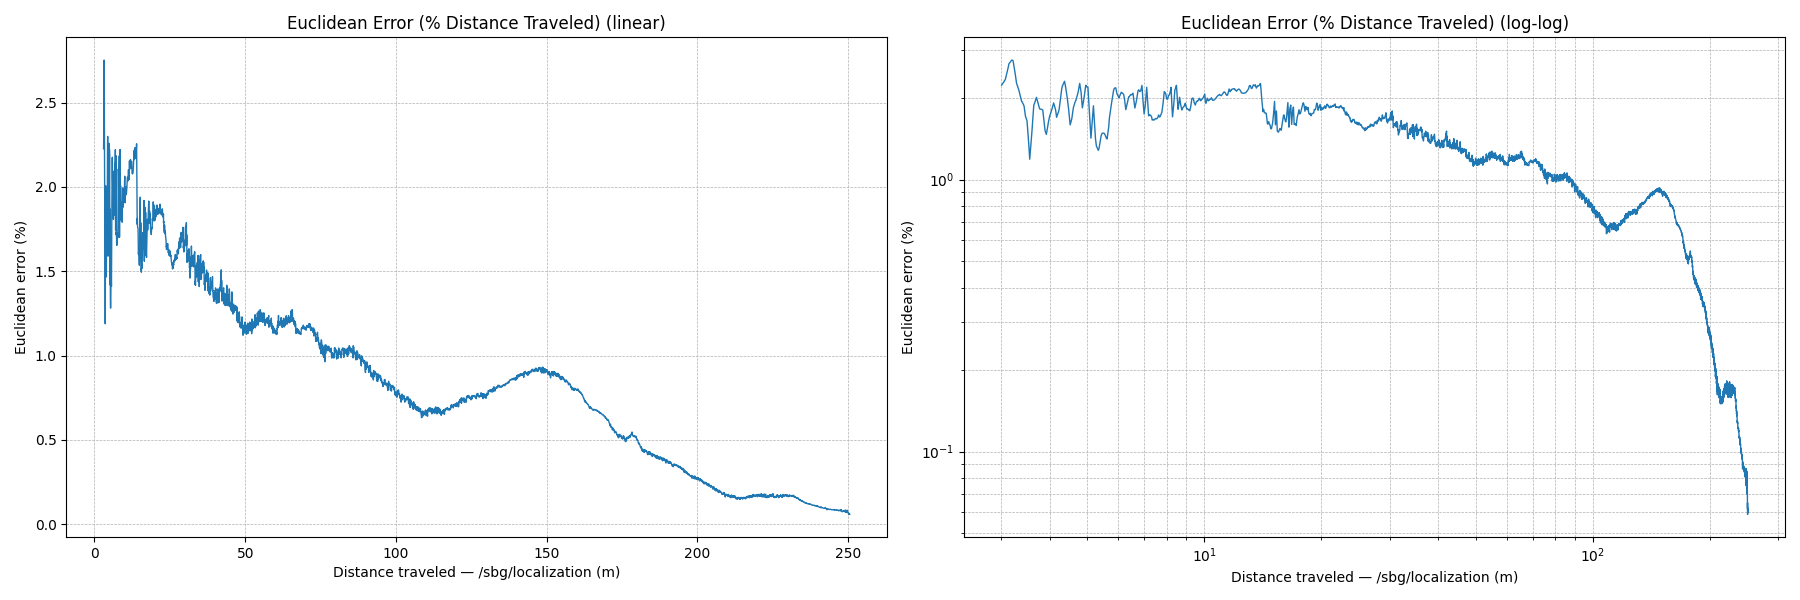
\includegraphics[width=1\linewidth]{Corps_rapport/euclidean_error_vs_distance.png}
    \captionof{figure}{Évolution de la dérive du SLAM DLIO par rapport à la vérité terrain en fonction de la distance parcourue}
    \label{fig35}
\end{center} 

Au regard de la figure ci-dessus, le SLAM DLIO présente une dérive particulièrement faible sur un parcours dégagé de 1 km, restant en dessous du seuil de 5 \% présenté par l'état de l'art dès 150 mètres parcourues. Ces résultats confirment définitivement son intégration pour la suite du challenge.\\

Afin d'évaluer l'adéquation des nouvelles fonctionnalités intégrées au module MOBILEX (notamment la navigation autonome reposant sur le SLAM DLIO) avec les exigences du défi 3 du challenge, un plan de test dédié a été conçu.

\subsubsection{Mise en place du plan de test}

Durant mon stage, il était attendu de moi la conception d'un plan de test rigoureux et reproductible afin d'évaluer les performances de la brique MOBILEX vis-à-vis des exigences du défi 3. Ce protocole vise à garantir la conformité des fonctionnalités du système avec les spécifications de la DGA, tout en assurant la répétabilité des essais, indépendamment de l'ingénieur chargé de leur exécution. Le terrain d'essais retenu pour le déroulement des tests est le site de l'INRAE Aubière du fait de sa proximité contrairement à celui de Montoldre. Il s'agissait ainsi de définir un ensemble de scénarios de test permettant la validation des exigences réglementaires fixées par la DGA (\hyperref[annexe3]{[règlementation DGA]}).\\

\indent À la suite d'échanges avec mon tuteur, nous avons opté pour le développement d'une carte géographique dynamique. Au sein de celle-ci, le positionnement des obstacles, des points de passage (waypoints) et des trajectoires s'adapte automatiquement au scénario sélectionné par l'opérateur. L'analyse topographique du terrain nous a permis d'identifier les zones propices au déroulement des différents essais. En nous appuyant sur des waypoints connus, nous avons délibérément choisi d'intégrer des obstacles (franchissables ou non) ainsi que des zones d'exclusion sur le site. Le résultat obtenu est illustré par la \hyperref[fig36]{Figure 36}.\\

\begin{center}
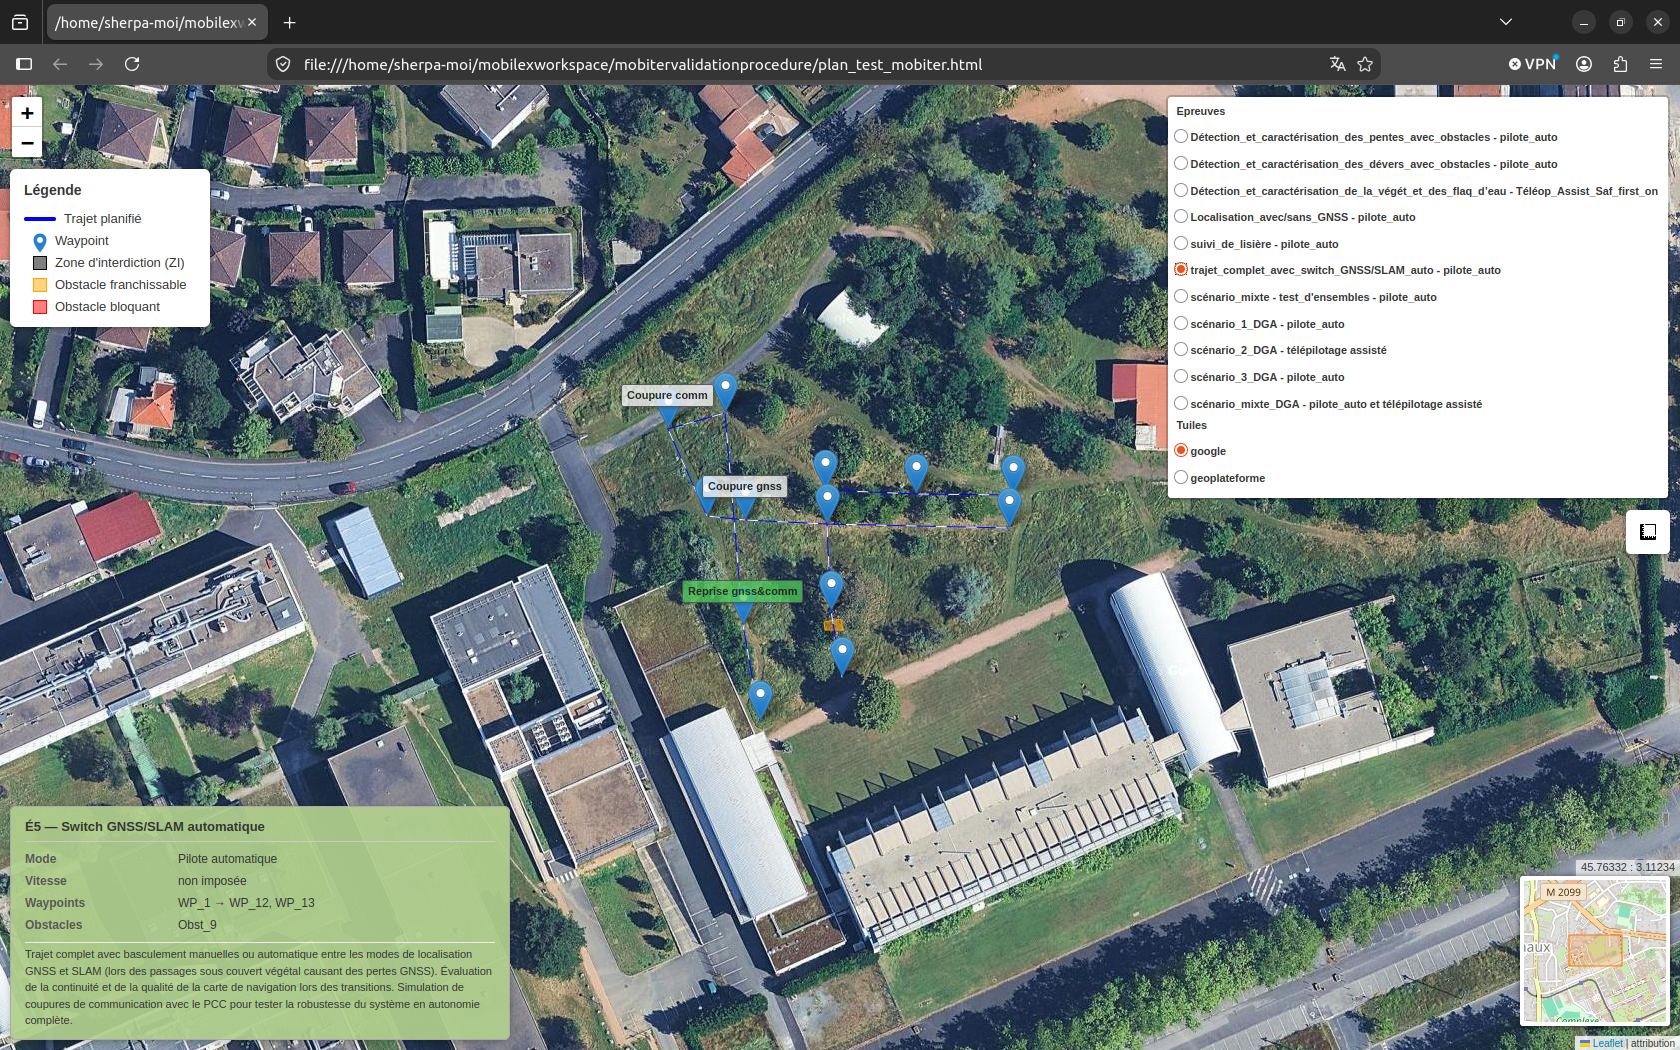
\includegraphics[width=1\linewidth]{Corps_rapport/plan_de_test_defi3.png}
\captionof{figure}{Plan de test graphique pour le défi 3}
\label{fig36}
\end{center} 

Cette carte dynamique a été développée en HTML et s'appuie sur la bibliothèque JavaScript Leaflet, dédiée à la création de cartes interactives. Elle permet de charger et d'afficher des données géospatiales issues de différentes sources, telles que des tuiles cartographiques ou des services de cartographie en ligne. L'interface utilisateur développée offre la possibilité de sélectionner divers scénarios de test ; la carte se met alors à jour automatiquement pour afficher les obstacles, les points de passage (waypoints) et les zones d'exclusion associés, tout en actualisant le descriptif de la mission dans la zone inférieure gauche.\\

\indent Une fois le plan de test graphique répétable établi, il a été nécessaire de mettre en place une checklist unique de propriétés à vérifier en ligne (lors du test) et hors ligne (après le test). Ce plan de test et cette checklist ont été conçus pour être utilisés par n'importe quel membre de l'équipe, garantissant ainsi la reproductibilité des tests et la comparaison des performances et résultats après chaque nouveau test. Elle comprend des points de contrôle précis subdivisé en 2 catégories: \\

\begin{itemize}
\renewcommand{\labelitemi}{$\bullet$}
    \item \textbf{Propriétés à vérifier en ligne} : Ces propriétés sont vérifiées en temps réel par l'opérateur lors de l'exécution du test. Elles incluent notamment la vérification de l'empatement du marquage au sol autour des waypoints, l'appui sur l'arrêt d'urgence durant le test, la reprise en téléopération du robot en cours de mission de suivi de waypoints, le ralentissement lors du franchissement d'obstacles ou de flaques d'eau ou de passage en mode SLAM, la perte de communication du robot avec le PCC, l'apparition d'accouts incessants lors du déplacement du robot et l'adéquation de la sémantique associée au retour vidéo de l'IHM avec l'environnement de test.
    \item \textbf{Propriétés à vérifier hors ligne} : Ces propriétés sont vérifiées après le test à partir des données enregistrées (ROS bag). Elles incluent notamment la vérification des trajectoires suivies par le robot, le respect des vitesses de commandes envoyées au robot, l'analyse de l'orientation (roll et pitch) du robot, et l'analyse des diagnostics émis sur l'IHM.\\
\end{itemize}

\indent Cette checklist présentée en annexe  \hyperref[annexe4]{[test\_checklist]} n'étant pas exhaustive, elle a été complétée par des points de contrôle pertinents supplémentaires en fonction des besoins et des observations faites lors des tests.\\

\indent Afin d'analyser efficacement les propriétés à vérifier hors ligne (après les essais), un générateur automatique de rapports a été développé. Cet outil synthétise les données d'exécution et fournit une analyse visuelle synthétique du déroulement des tests, facilitant ainsi le diagnostic et la prise de décision.\\

\subsubsection{Mise en oeuvre du générateur automatique de rapports d'essais}

L'une de mes missions principales a été de développer un générateur automatique de rapports d'essais. Cet outil vise à synthétiser les données d'exécution des tests pour fournir une analyse visuelle et rapide du déroulement des essais afin de faciliter les diagnostics.\\\\
\indent Le générateur de rapports d'essais a été conçu pour assurer un traitement offline des fichiers de données (ROS bag) enregistrés lors des tests. Il extrait les informations pertinentes, telles que les trajectoires, les vitesses, les erreurs de localisation, les événements critiques, les images de cartes construites et de visualisation, puis génère un rapport structuré comprenant des graphiques, des informations de diagnostic et des vidéos.\\\\
\indent Apres discussion avec l'ensemble de l'équipe, une liste d'éléments pertinents à inclure dans le rapport de test a été établie. Cette liste comprend notamment:\\

\begin{itemize}
\renewcommand{\labelitemi}{$\bullet$}
    \item La liste des diagnostics (avec timestamps) retournés sur l'IHM durant toute la durée des tests : sous forme de figure facilement interpretable puis sous forme de test plus descriptif contenant le message d'erreur associé à chaque disgnostic.
    \item Le mode de control du robot (téléopération, suivie de waypoint, ...) ainsi que le mode de localisation (GNSS, SLAM) du robot à chaque timestamps sous forme de figure.
    \item Un tracé des positions linéaires et angulaires du robot.
    \item Un tracé de la trajectoire du robot en slam et en GNSS RTK avec les waypoints à raliés, ainsi qu'une évaluation des erreurs de localisation.
    \item Un tracé de la trajectoire du robot avec les waypoints à raliés ainsi qu'une representation du mode de localisation sur chaque section de la trajectoire.
    \item Un tracé des erreurs de vitesses linéaires sur toute la tarjectoire par rapport aux vitesses de consigne souhaitée.
    \item Des vidéos synchronisées par rapport aux timestamps des bag, montrant la construction du MNE(Modele Numerique d'Elevation), de la planification globale, de la planification locale, de la carte des gradients ainsi que du retour vidéo sur l'IHM.\\
\end{itemize}

\indent L'outil a été développé en Python et utilise des bibliothèques telles que Matplotlib pour la visualisation des données, Pandas pour le traitement des données et OpenCV pour la manipulation d'images et de vidéos. A partir du bag ROS, le rapport final est généré au format html sous demande des membres de l'équipe. L'organigramme de l'outil est présenté dans la (\hyperref[fig37]{Figure 37}):\\

\begin{center}
    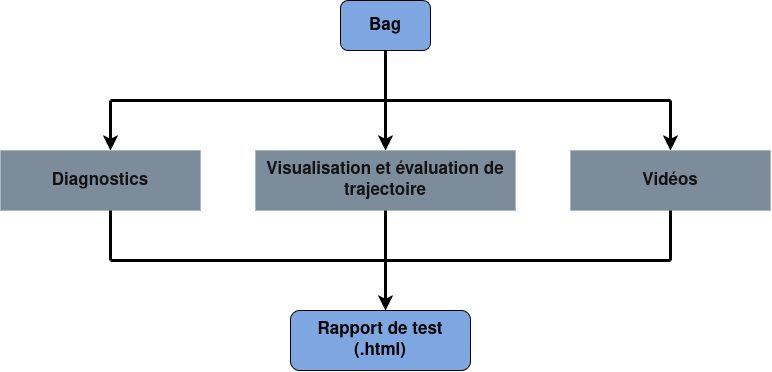
\includegraphics[width=0.8\linewidth]{Corps_rapport/org_bag_explorer.png}
    \captionof{figure}{Organigramme de l'outil de génération automatique de rapport de test}
    \label{fig37}
\end{center}

\paragraph{Extraction et génération des diagnostics de l'IHM}

L'objectif principal de ce module est d'obtenir une vision consolidée et exhaustive de l'ensemble des diagnostics émis par l'interface homme-machine (IHM) sur la totalité de la plage temporelle de l'essai. Cette approche permet notamment de capturer et de consigner les événements transitoires (des alertes fugaces qui apparaissent et disparaissent rapidement), évitant ainsi qu'ils ne soient omis par l'opérateur lors du déroulement du test en temps réel.\\

\indent Le processus débute par l'analyse du fichier d'enregistrement (bag file), dont l'objectif est d'extraire l'ensemble des topics de type \textbf{DiagnosticArray}. Si une liste restrictive de topics est fournie en paramètre, l'extraction se limite à ces derniers ; dans le cas contraire, l'intégralité des flux de type DiagnosticArray est récupérée par défaut. Une fois l'extraction effectuée, les informations utiles sont structurées et stockées chronologiquement au sein d'un dictionnaire indexé par horodatage (timestamp). À partir de cette structure de données, des scripts exploitant des library Python (pandas, numpy, matplotlib) génèrent automatiquement l'ensemble des figures d'analyse présentées précédemment, ainsi qu'un rapport de synthèse textuel (format .txt). De plus, afin de mettre en relation les anomalies matérielles ou logicielles avec l'état opérationnel du robot, l'outil extrait également les messages du topic \textbf{nav\_stack/control\_mux/mode}. L'analyse de ce topic permet de tracer et de corréler précisément les changements de modes de contrôle du système au cours de l'essai. Enfin, l'outil donne également un rapide aperçu des fréquences de publication des topics du bag par rapport celles de réference, permettant ainsi d'identifier les éventuels problèmes de communication ou de perte de données. La figure (\hyperref[fig38]{Figure 38}) suivante illustre l'organigramme de cet outil d'extraction de diagnostic:\\
 
\begin{center}
    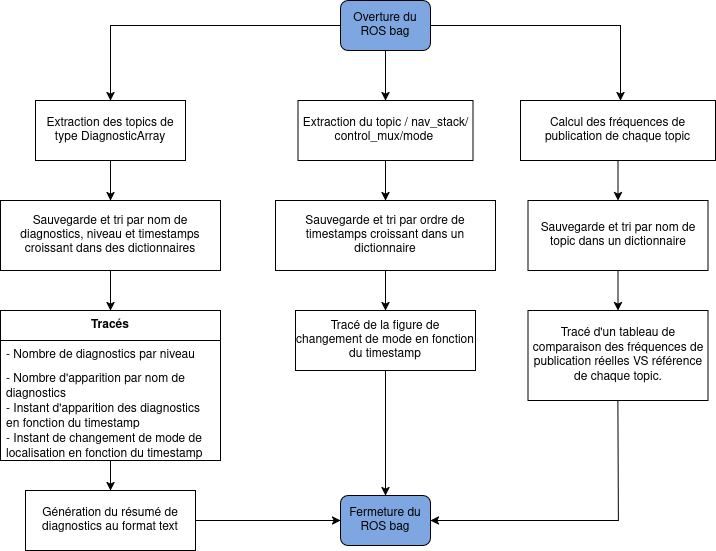
\includegraphics[width=0.7\linewidth]{Corps_rapport/org_diag_extractor.png}
    \captionof{figure}{Organigramme de l'outil d'extraction et de génération des diagnostics}
    \label{fig38}
\end{center}

\indent Comme résultat, l'outil génère plusieurs représentations graphiques, dont une frise chronologique (timeline) des diagnostics (\hyperref[fig39]{Figure 39}), indexée par identifiant d'alerte. Cette visualisation temporelle permet d'identifier immédiatement les éléments où des anomalies sont survenues, puis de fournir un résumé sur ces diagnostics anormaux détectés. Au sein de la pile logicielle (stack) MOBITER, les diagnostics sont hiérarchisés et catégorisés en quatre grands groupes fonctionnels (niveau) :\\

\begin{itemize}
\renewcommand{\labelitemi}{$\bullet$}
    \item \textbf{OK} : qui indique que tout fonctionne correctement.
    \item \textbf{WARNING} : qui indique un avertissement ou un problème potentiel.
    \item \textbf{ERROR} : qui indique une erreur nécessitant une attention immédiate.
    \item \textbf{STALE} : qui indique que les informations ne sont plus à jour.\\
\end{itemize}

\begin{center}
    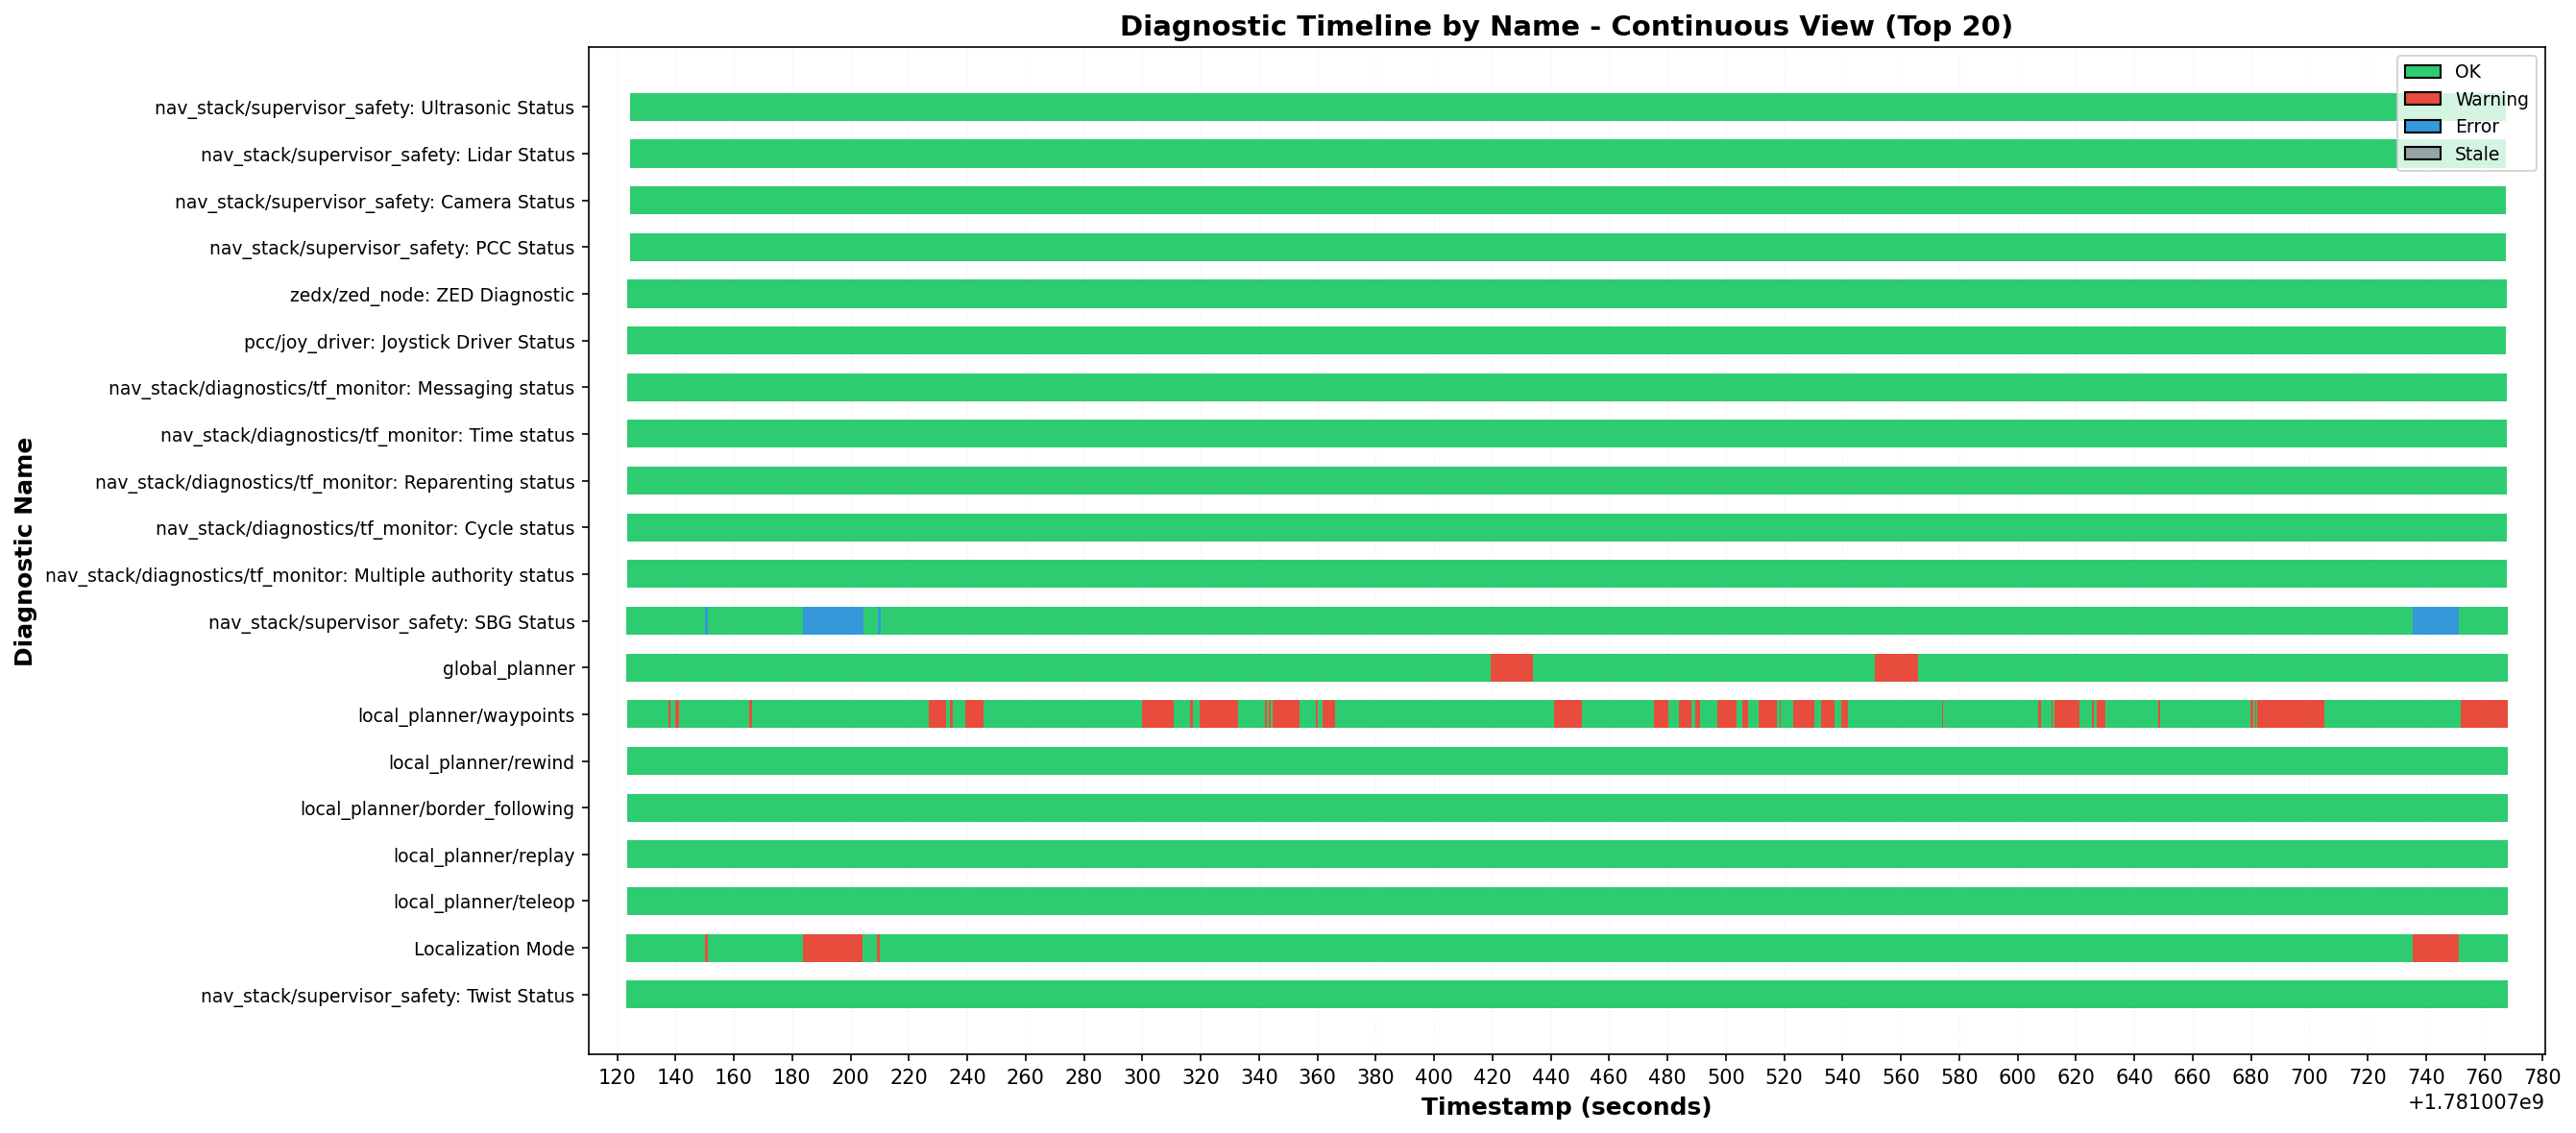
\includegraphics[width=1\linewidth]{Corps_rapport/diagnostics_timeline_by_name.png}
    \captionof{figure}{Timeline des diagnostics de l'IHM par nom de diagnostic}
    \label{fig39}
\end{center}

\indent Deplus, pour des soucis de débug il est souvent interessant de savoir à quel moment le robot a changé de mode de contrôle (téléopération, suivis de waypoint, suivis de lisiere) ou de localisation (GNSS ou SLAM). L'outil génère donc également des timelines de ces changements de mode de contrôle et de localisation (\hyperref[fig40]{Figure 40} et \hyperref[fig41]{Figure 41}).\\

\begin{center}
    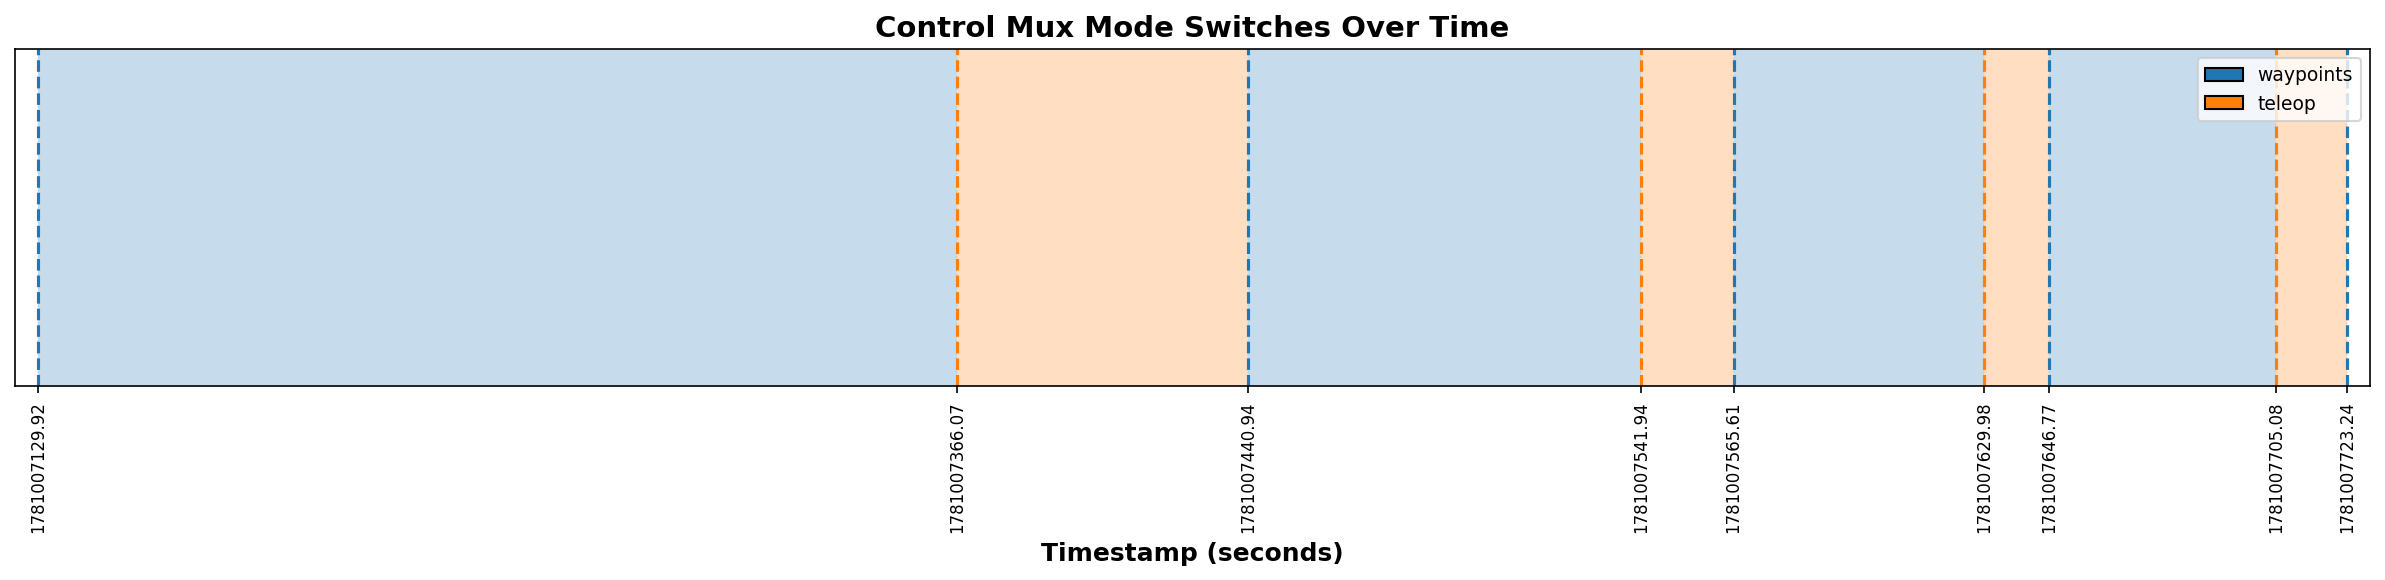
\includegraphics[width=1\linewidth]{Corps_rapport/control_mode_switches.png}
    \captionof{figure}{Timeline des changements de mode de contrôle}
    \label{fig40}
\end{center}

\indent Pour le cas de test illustré en \hyperref[fig40]{Figure 40}, on observe que l'opérateur a repris la main sur le robot en mode téléopération à 4 reprises durant le suivi de waypoints. Cela pourrait traduire une difficulté pour le robot à rallier certains points de passage en toute autonomie.\\

\begin{center}
    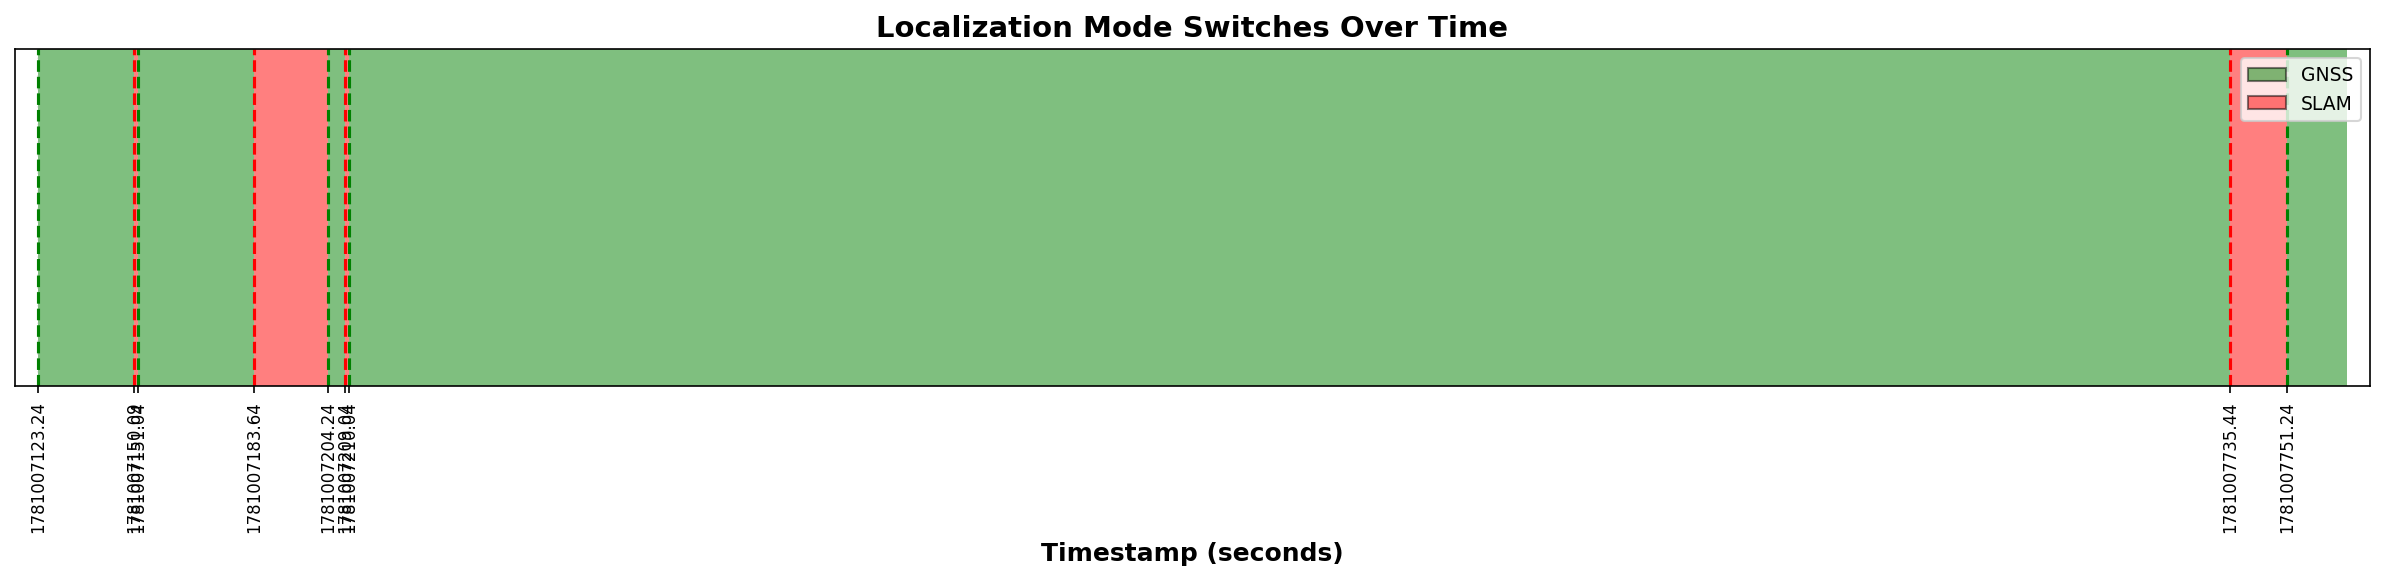
\includegraphics[width=1\linewidth]{Corps_rapport/localization_mode_switches.png}
    \captionof{figure}{Timeline des changements de mode de localisation}
    \label{fig41}
\end{center}

\indent Concernant le cas de test illustré par la \hyperref[fig41]{Figure 41}, on observe que le robot a changé de mode de localisation à 4 reprises durant le suivi de waypoints. Cela pourrait traduire plusieurs passages sous couvert végétal le long du trajet.


\paragraph{Extraction et génération des visualisation de trajectoires et d'erreurs de localisation}

Ce module a pour objectif principal de fournir une représentation visuelle et quantitative des trajectoires du robot (estimées par le SLAM et la centrale inertielle SBG Ellipse) au regard des waypoints (points de passage) à rallier. Afin d'évaluer et de comparer objectivement ces profils de déplacement, la bibliothèque Python EVO a été intégrée à l'architecture de test. L'outil automatisé exploite cette bibliothèque pour générer plusieurs types de livrables graphiques :\\

\begin{itemize}
\renewcommand{\labelitemi}{$\bullet$}
    \item \textbf{Des analyses temporelles} : l'évolution des positions linéaires et angulaires du robot au fil du temps.(\hyperref[fig43]{Figure 43})
    \item \textbf{Des comparaisons spatiales} : la superposition des trajectoires issues du SLAM et de la centrale inertielle SBG.(\hyperref[fig44]{Figure 44})
    \item  \textbf{Des métriques d'erreur} : le calcul et l'affichage de l'erreur de position relative (RPE — Relative Pose Error) pour quantifier la dérive locale du système.\\
\end{itemize}

\indent Afin d'optimiser le traitement, l'architecture de cet outil a été subdivisée en deux modules distincts :\\

\begin{itemize}
\renewcommand{\labelitemi}{$\bullet$}
    \item Le module d'extraction et de sérialisation : Cette première partie est chargée d'extraire les informations pertinentes des topics du fichier bag, puis de les enregistrer dans un fichier CSV. Les données y sont structurées sous forme de tableau indexé par horodatage (timestamp), où chaque colonne correspond à un attribut spécifique et exploitable du message d'origine.
    \item Le module d'analyse et de visualisation : Cette seconde partie assure la lecture du fichier CSV et prend en charge la génération des différentes figures d'analyse.\\
\end{itemize}

\indent Cette conception modulaire et découplée présente un double intérêt opérationnel. D'une part, elle évite de réexécuter la phase d'extraction des données du bag (processus qui peut etre lourd et chronophage) lors d'un simple ajustement graphique ou d'une modification des figures d'analyse. D'autre part, elle permet de générer un fichier CSV intermédiaire. Ce support, considérablement plus léger qu'un fichier bag, assure la persistance de données pré-traitées et exploitables pour des analyses ultérieures.\\

\indent Pour la première partie du traitement, l'outil génère ainsi un fichier CSV indexé par horodatage contenant les colonnes associées aux différents champs des messages pour les topics de type :\\

\begin{itemize}
\renewcommand{\labelitemi}{$\bullet$}
    \item \textbf{geometry\_msgs/TwistStamped} : Champ linéaire et angulaire de la vitesse afin d'avoir les vitesses de consigne envoyées au robot à chaque instant
    \item \textbf{nav\_msgs/Odometry} : Pose du robot dans les différents modes de localisation (SLAM, SBG) pour des tracés de trajectoires.
    \item \textbf{nav\_msgs/Path} : Liste et coordonnées des waypoints à rallier par le robot pour les tracés sur trajectoires.
    \item \textbf{sensor\_msgs/Imu} : Mesures inertielle pour les tracés d'orientation du robot tout au long de la trajectoire.
    \item \textbf{diagnostic\_msgs/DiagnosticArray} : Diagnostics de l'IHM pour l'identification des changements de mode de localisation afin de les superposer sur les tracés de trajectoires.\\ 
\end{itemize} 

\indent Pour la seconde partie du traitement, l'outil exploite les données du CSV pour générer une série de visualisations détaillées, complétée par des métriques d'évaluation standardisées. Ces livrables graphiques se divisent en deux catégories principales :

\subparagraph{a. Les figures d'analyse dynamique et comportementale}:

Ces tracés permettent de caractériser finement le comportement cinématique et l'état du système tout au long de son parcours : \\

\begin{itemize}
\renewcommand{\labelitemi}{$\bullet$}
    \item \textbf{Analyse spatiale et trajectographie} : Superposition et comparaison des trajectoires estimées par le SLAM et par la centrale inertielle (SBG Systems), avec projection des points de passage (waypoints) cibles.
    \item \textbf{Modes de localisation} : Visualisation temporelle et géographique du mode de localisation actif (SLAM ou GNSS RTK) sur les différentes portions de la trajectoire.(\hyperref[fig44]{Figure 44})
    \item \textbf{Attitude du châssis} : Évolution des angles d'orientation de roulis (roll) et de tangage (pitch) du robot le long de la trajectoire, permettant d'identifier d'éventuelles orientations dangereuses liées au relief.
    \item \textbf{Suivi de consigne en vitesse} : Confrontation des vitesses linéaires et angulaires de consigne avec les vitesses réelles mesurées sur le robot.
    \item \textbf{Analyse des écarts de vitesse} : Évaluation des erreurs de vitesse instantanées par rapport aux vitesses de consigne requises pour le ralliement des waypoints.(\hyperref[fig44]{Figure 44})
    \item \textbf{Performances temporelles du suivi} : Mesure fine de la durée de ralliement pour chaque waypoint intermédiaire, ainsi que le calcul du temps total d'exécution de la mission de suivi de trajectoire.
\end{itemize}

\subparagraph{b. Les figures d'évaluation géométrique de la trajectoire}:

En complément de ces analyses comportementales, l'outil intègre un module d'évaluation métrologique s'appuyant sur la bibliothèque EVO. Ce module génère automatiquement des figures d'évaluation standardisées, permettant notamment de quantifier l'erreur de pose absolue (APE - Absolute Pose Error) et l'erreur relative de pose (RPE - Relative Pose Error) par rapport à la trajectoire de référence comme présenté dans la section 2.3.\\

\indent Le processus débute par l'analyse du fichier d'enregistrement (bag file), dont l'objectif est d'extraire et de sauvegarder dans un CSV les valeurs des champs d'un ensemble de topics : \\

\begin{itemize}
\renewcommand{\labelitemi}{$\bullet$}
    \item \textbf{/dlio/dlio\_odom/transformed\_slam\_pose} et \textbf{/sbg/localization} : Pour la localisation SLAM et GNSS du robot.
    \item \textbf{/nav\_stack/function\_waypoints/waypoints\_iterator/path\_in} : Pour l'ensemble des waypoints à rallier par le robot.
    \item \textbf{/barakuda/cmd\_vel} : Pour les commandes / consignes en vitesses envoyées au robot.
    \item \textbf{/main\_odometry} : Pour extraire les vitesses réelles suivies par le robot peu importe le mode de localisation.
    \item \textbf{/nav\_stack/function\_waypoints/waypoints\_iterator/next\_waypoint\_speed} : Pour extraire les vitesses de consigne souhaitées par le robot pour le ralliement des waypoints.
    \item \textbf{/sherpa\_board/xsens\_mti/imu} : Pour extraire les angles d'orientation du robot (roulis et tangage) à chaque instant.
    \item \textbf{/diagnostics} : Pour extraire les diagnostics de l'IHM et identifier les changements de mode de localisation.\\
\end{itemize}

Une fois le CSV généré, l'outil exploite ces données pour produire automatiquement des figures resultant de tracé de colonnes vs colonnes ou de colonnes vs timestamps, ainsi que des figures d'évaluation standardisées (APE et RPE) à l'aide de la bibliothèque EVO. Ces visualisations permettent d'obtenir une vue d'ensemble du comportement du robot, de ses performances de localisation et de son suivi de trajectoire, facilitant ainsi l'identification des anomalies et l'optimisation des algorithmes de navigation. La figure (\hyperref[fig42]{Figure 42}) suivante illustre l'organigramme de cet outil:

\begin{center}
    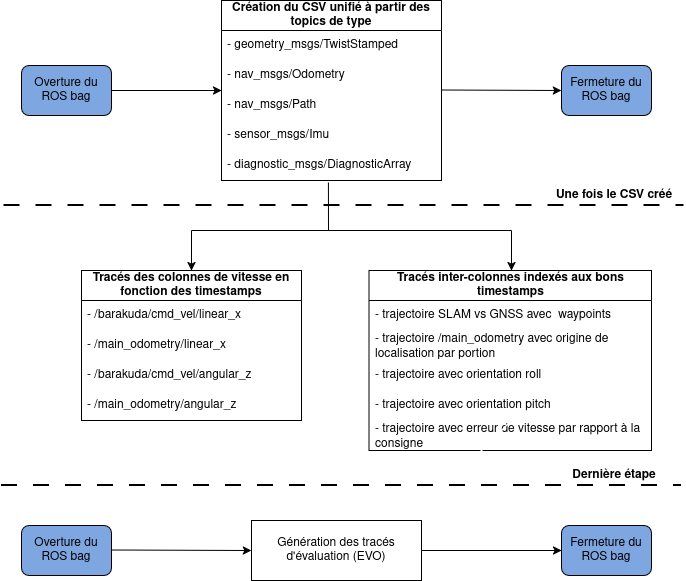
\includegraphics[width=0.7\linewidth]{Corps_rapport/org_viz_extractor.png}
    \captionof{figure}{Organigramme de l'outil d'extraction et de génération des visualisations}
    \label{fig42}
\end{center}
$\ $\

Comme résultat, l'outil génère plusieurs graphiques dont les figures (\hyperref[fig43]{Figure 43} et \hyperref[fig44]{Figure 44}) suivantes :\\

\begin{figure}[H]
    \centering
    \begin{subfigure}[b]{0.46\textwidth}
        \centering
        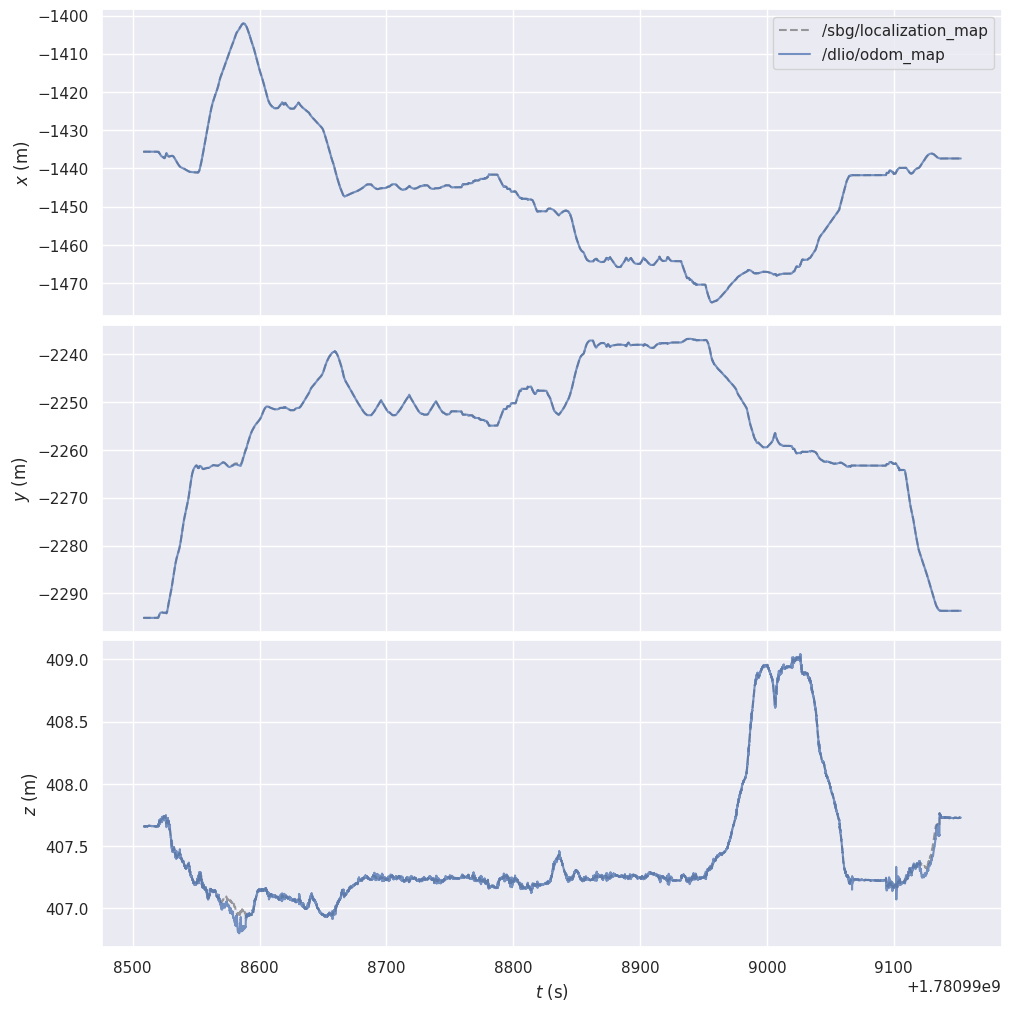
\includegraphics[width=\textwidth]{Corps_rapport/evo_trajectory_analysis_xyz.png}        
    \end{subfigure}
    \hfill
    \begin{subfigure}[b]{0.46\textwidth}
        \centering
        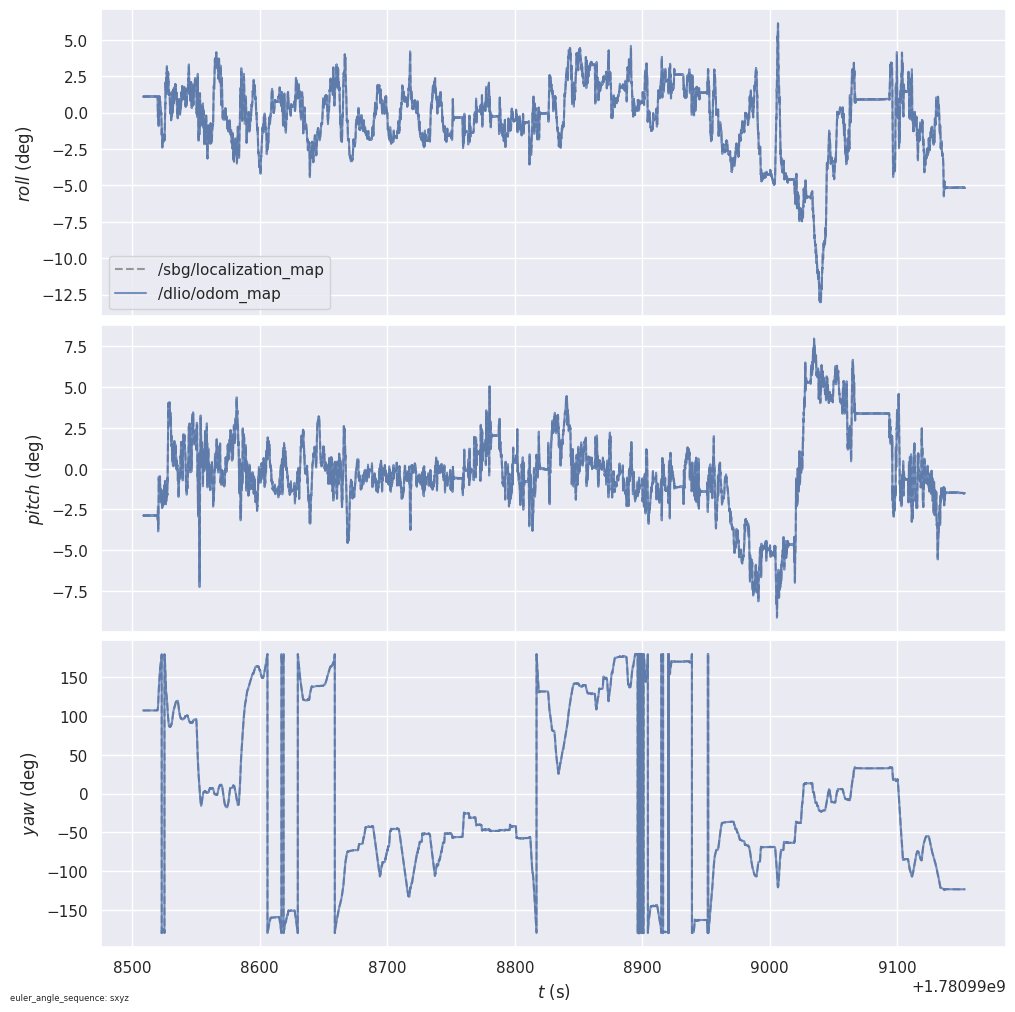
\includegraphics[width=\textwidth]{Corps_rapport/evo_trajectory_analysis_rpy.png}
    \end{subfigure}
    \caption{Visualisation et comparaison des positions linéaires et angulaires du robot}
    \label{fig43}
\end{figure}

\indent La figure \hyperref[fig43]{Figure 43} illustre la très bonne estimation de la pose du robot par le SLAM DLIO par rapport à la vérité terrain fournie par la centrale SBG. On observe que les positions linéaires et les orientations angulaires estimées par le SLAM sont très proches de celles mesurées par la centrale inertielle, ce qui confirme la précision et la fiabilité du SLAM DLIO pour la navigation.

\begin{figure}[H]
    \centering
    \begin{subfigure}[b]{0.46\textwidth}
        \centering
        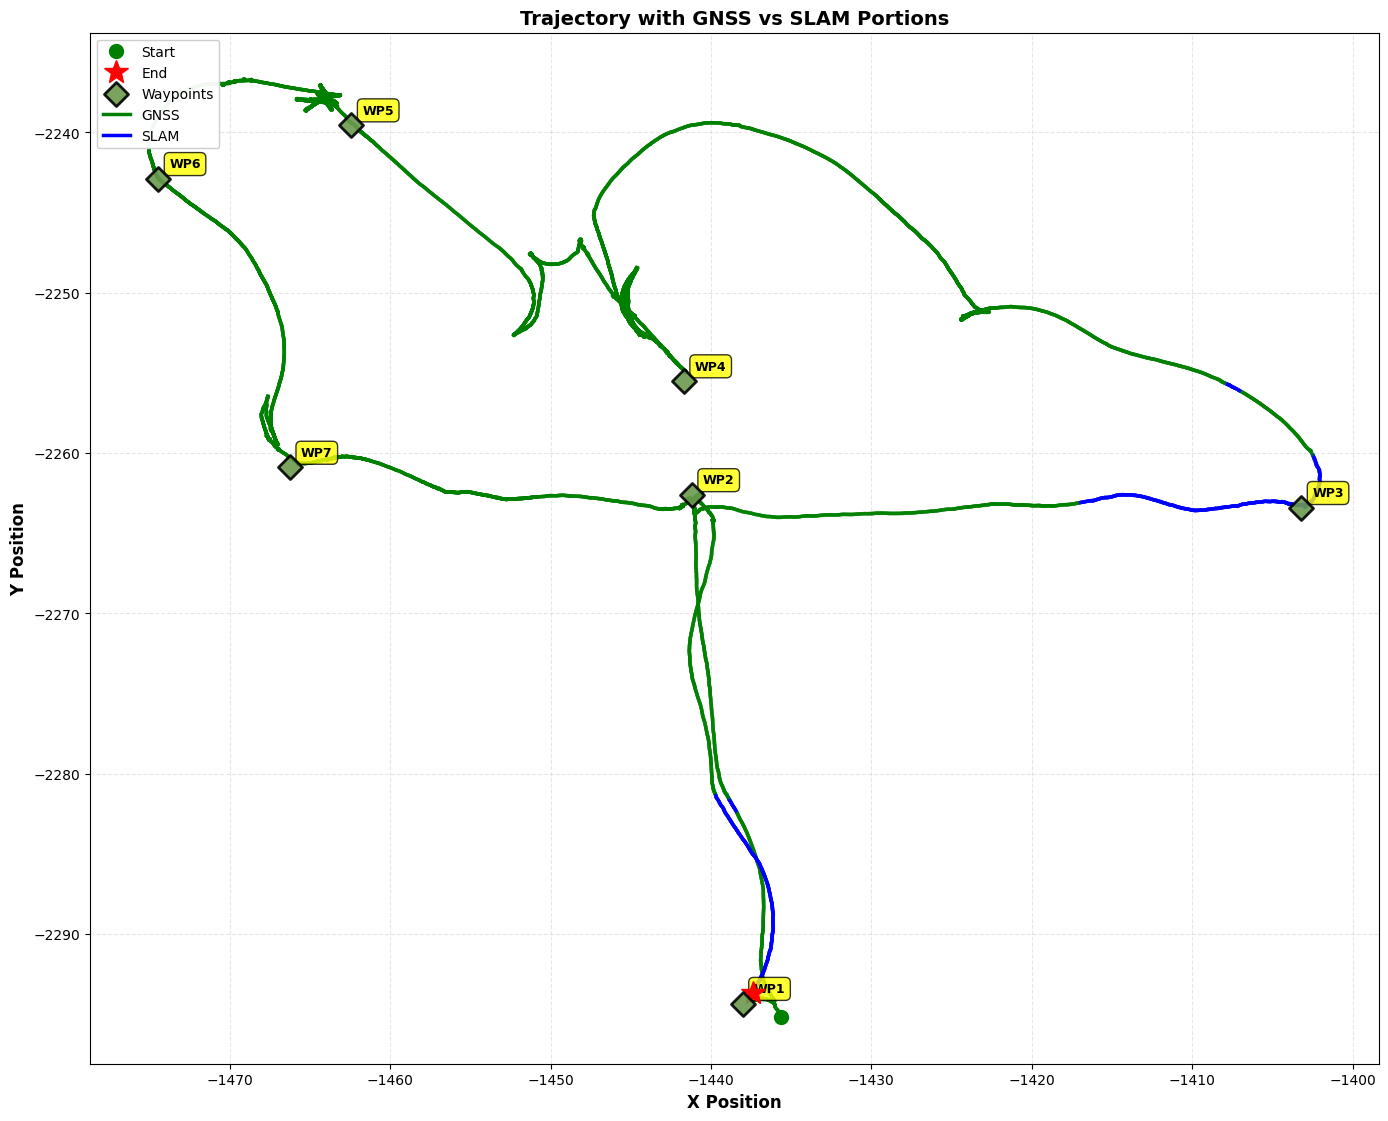
\includegraphics[width=\textwidth]{Corps_rapport/trajectory_gnss_vs_slam.png}        
    \end{subfigure}
    \hfill
    \begin{subfigure}[b]{0.5\textwidth}
        \centering
        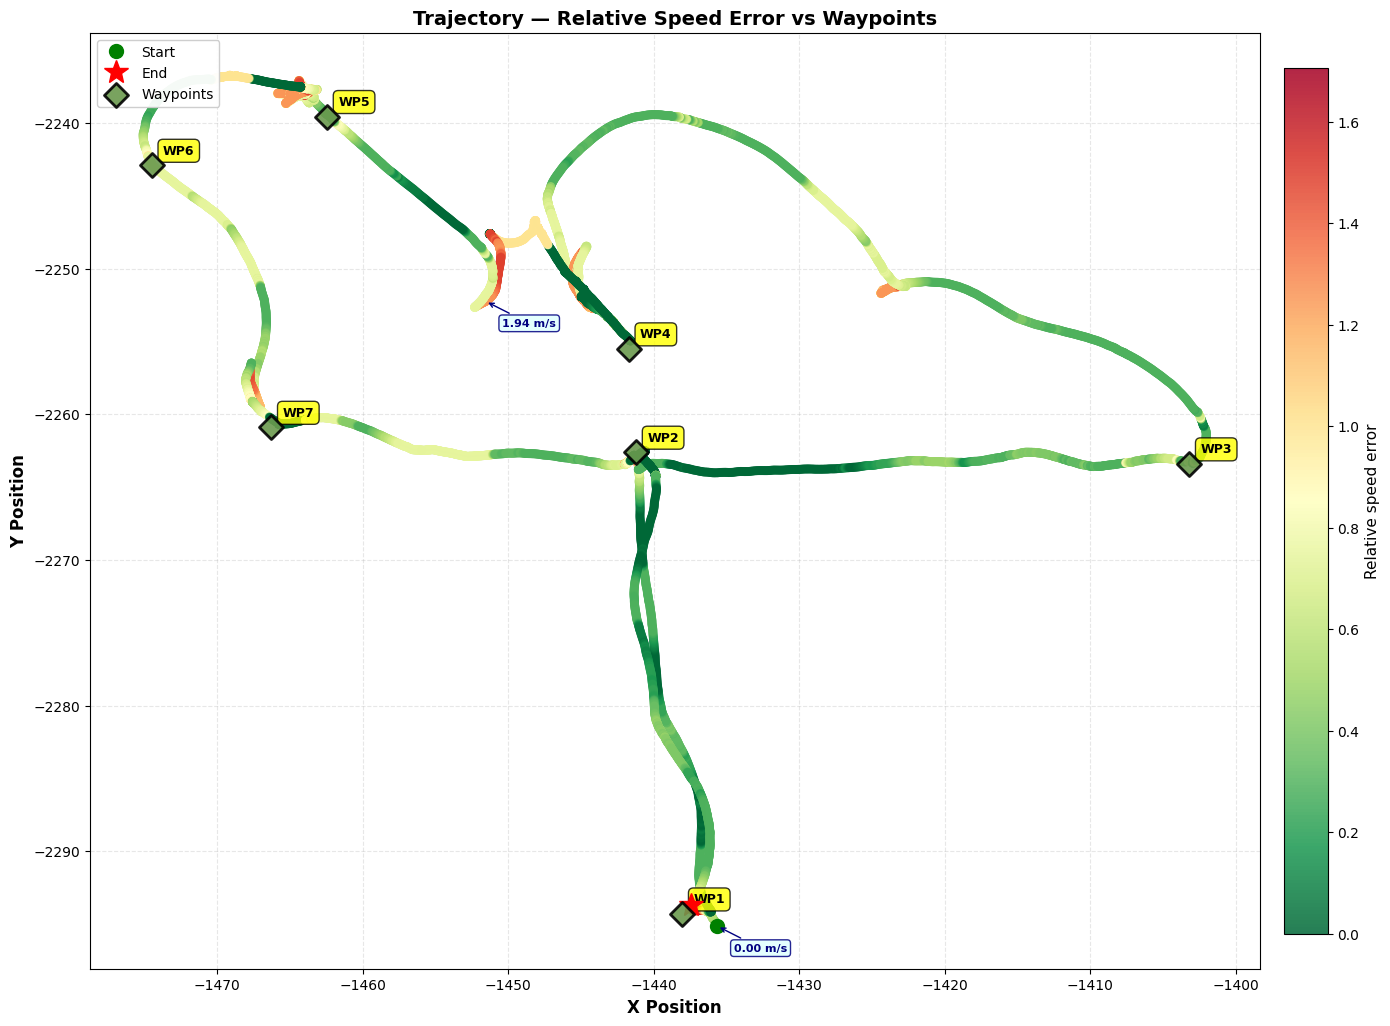
\includegraphics[width=\textwidth]{Corps_rapport/trajectory_speed_error.png}
    \end{subfigure}
    \caption{Evaluation des portions GNSS et SLAM de la trajectoire et erreur de vitesse le long de la trajectoire}
    \label{fig44}
\end{figure}
 
\indent La figure \hyperref[fig44]{Figure 44} met en évidence les portions de la trajectoire où le SLAM DLIO a été utilisé pour la localisation, ainsi que celles où le GNSS RTK a été employé. Elle pourra être comparée à la carte de végétation du site afin de vérifier que les zones de basculement automatique vers le SLAM correspondent effectivement aux zones de couvert. De plus, cette figure illustre les écarts de vitesse le long du parcours, permettant d'identifier les zones de fort ralentissement.\\

\indent Ces visualisations synthétiques permettent d'identifier rapidement les écarts géométriques entre les différentes méthodes de localisation et d'analyser finement les performances de la brique de navigation selon les scénarios de test. Il convient toutefois de souligner que la pertinence de ces indicateurs de performance (KPI) reste conditionnée à la validité de la vérité terrain (ground truth). Celle-ci nécessite une continuité absolue des données de positionnement, ce qui implique l'absence de masquage ou de perte du signal GNSS RTK durant l'acquisition des données.\\


\paragraph{Extraction et génération des vidéos de l'évolution des cartes et du retour vidéo sur l'IHM}

Ce module a pour objectif principal de fournir une représentation visuelle dynamique (vidéo) de l'évolution du MNE (Modèle Numérique d'Élévation), de la planification globale et locale, ainsi que du retour vidéo affiché sur l'interface homme-machine (IHM). S'il n'est pas spécifié de topic particulier en paramètre, l'outil automatise l'extraction des données de l'ensemble des topics \textbf{sensor\_msgs/Image} et \textbf{sensor\_msgs/CompressedImage} présents dans le rosbag. Après décodage des trames, une vidéo synchronisée est générée pour chaque topic au moyen de la bibliothèque OpenCV. Les différents topics d'images ne publiant pas à la même fréquence, l'outil effectue un rééchantillonnage temporel basé sur le timestamp des messages. Un pas temporel commun est calculé en se basant sur le topic possédant la fréquence d'échantillonnage la plus basse. Ainsi, selon leur fréquence d'origine, certains topics ne conservent qu'une image sur deux, voire une image sur quatre pour l'assemblage de leur vidéo respective. Afin d'aligner le début et la fin de l'ensemble des vidéos générées, un offset temporel est appliqué. Ce timestamp d'origine est déterminé par le topic d'image dont la première publication est la plus tardive ; toutes les trames antérieures à cet offset sont ignorées. L'outil génère ainsi un ensemble de vidéos parfaitement synchronisées. Enfin, ces flux sont unifiés au sein d'une vidéo composite par un assemblage image par image (frame-by-frame).  La figure (\hyperref[fig45]{Figure 45}) suivante illustre l'organigramme de cet outil:\\

\begin{center}
    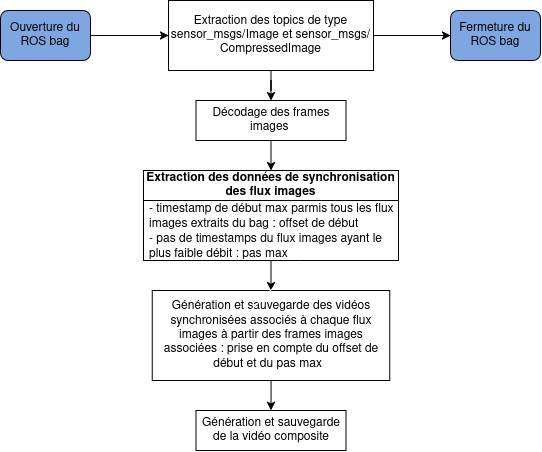
\includegraphics[width=0.7\linewidth]{Corps_rapport/org_video_extractor.png}
    \captionof{figure}{Organigramme de l'outil d'extraction et de génération de vidéos}
    \label{fig45}
\end{center}

\indent La figure (\hyperref[fig46]{Figure 46}) suivante illustre un exemple de vidéo composite générée par l'outil, montrant l'évolution des cartes et du retour vidéo sur l'IHM. Cette vidéo composite offre ainsi une vue d'ensemble du comportement du système durant les essais et permet d'observer, dans l'ordre de lecture (de gauche à droite et de haut en bas) :\\

\begin{itemize}
\renewcommand{\labelitemi}{$\bullet$}
    \item la planification globale de trajectoire. 
    \item la planification locale de trajectoire. 
    \item la carte des gradients d'élévation autour du robot. 
    \item le MNE (Modèle Numérique d'Élévation). 
    \item la visualisation LiDAR.
    \item la vue annotée de l'IHM. \\
\end{itemize}

\begin{center}
    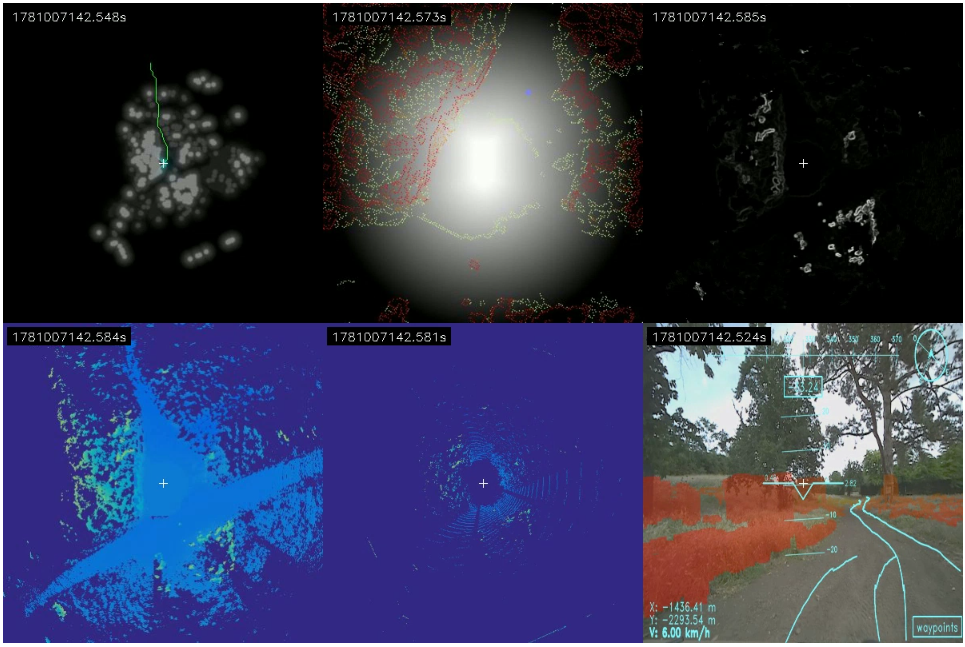
\includegraphics[width=0.7\linewidth]{Corps_rapport/video_aggra.png}
    \captionof{figure}{Vidéo composite des différentes cartes et du retour vidéo sur l'IHM}
    \label{fig46}
\end{center}


\paragraph{Structuration modulaire du générateur de rapports}

\indent Une fois le générateur de rapports de test rendu fonctionnel, l'objectif suivant a consisté à lui apporter une structure modulaire. Cette modularité devait permettre à l'utilisateur de sélectionner à la carte les informations à intégrer dans le rapport final, parmi les options suivantes : diagnostics, visualisation de trajectoires et vidéos. Pour ce faire, j'ai suivi les recommandations d'un ingénieur de l'équipe et me suis tourné vers les bibliothèques Rich et Typer. Rich permet d'améliorer l'affichage dans le terminal, rendant l'expérience utilisateur plus attrayante, tandis que Typer facilite la création d'applications en ligne de commande avec la possibilité de passer des arguments pour spécifier les éléments à générer dans le rapport. L'outil se presente comme le montre la figure suivante (\hyperref[fig47]{Figure 47}):\\
 
\begin{center}
    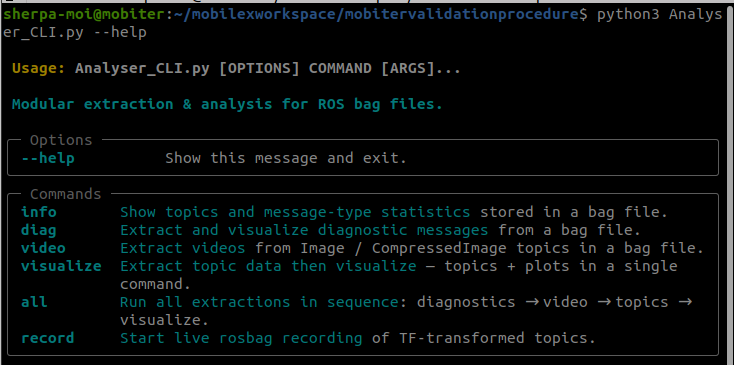
\includegraphics[width=0.7\linewidth]{Corps_rapport/presentation_outil_extraction.png}
    \captionof{figure}{Visualisation terminal de l'outil de génération automatique de rapport de test}
    \label{fig47}
\end{center}


















\subsubsection{Proposition de méthode d'automatisation de la validation de tests en robotique mobile: cas d'application sur Mobiter}

La validation des systèmes autonomes (robots agricoles, drones, véhicules autonomes, robots sous-marins) repose traditionnellement sur des expérimentations sur le terrain. Bien qu'indispensables, ces essais réels présentent de fortes contraintes : un coût financier élevé, des risques matériels et humains, ainsi qu'une répétabilité limitée en raison de la variabilité des conditions environnementales.  

Pour répondre à ces limites, le test en simulation s'est imposé comme une démarche complémentaire majeure. Il permet d'exécuter de façon intensive des suites de tests à moindre coût et en toute sécurité. Les architectures logicielles de simulation se déclinent principalement sous trois formes :  \\

\begin{itemize}
    \item Model-in-the-Loop (MiL) : vérification précoce sur des modèles abstraits (ex. Simulink).
    \item Software-in-the-Loop (SiL) : intégration du logiciel embarqué réel dans un environnement virtuel simulant capteurs et actionneurs.
    \item Hardware-in-the-Loop (HiL) / Vehicle-in-the-Loop (ViL) : exécution sur le matériel physique connecté à des composants virtuels.\\
\end{itemize}

L'automatisation complète de la chaîne de validation soulevait trois verrous scientifiques et techniques fondamentaux : la spécification d'un oracle de test automatisé, la génération de cas de test contraints et variés, et la prise en compte du non-déterminisme.

\paragraph{Méthode basée sur la spécification et l'automatisation des oracles de test}

Le problème de l'oracle de test consiste à déterminer automatiquement si le comportement observé lors d'une exécution correspond au comportement attendu. En robotique autonome, la définition d'un oracle est complexe en raison de l'effet « boule de neige » des décisions logicielles, du volume massif de données produites et de l'absence de spécification complète.

\subparagraph{Oracles basés sur des invariants et propriétés de sûreté}:

Pour contourner la difficulté de prédiction exacte de la trajectoire d'un robot, une approche privilégiée consiste à définir des oracles spécifiés reposant sur des invariants fonctionnels et de sécurité.\cite{2021TOU30119b}  \\

Dans les travaux portant sur le robot agricole Oz et le robot sous-marin REMI, les oracles ont été formalisés autour d'une classification de propriétés :  \\

\begin{itemize}
    \item Propriétés liées aux phases de mission : contrôle du respect de la séquence d'étapes (ex. suivi de ligne, manœuvre de demi-tour, transition vers l'inter-rang suivant).
    \item Seuils physiques et cinématiques : vérification des vitesses maximales, des angles de braquage ou des accélérations par rapport aux limites de sécurité fixées.
    \item Événements catastrophiques et sécurité : détection de collisions, franchissement des limites du terrain, déclenchement inapproprié des arrêts d'urgence ou dépassement des seuils de batterie.
    \item Gestion des erreurs et perception : vérification de la cohérence des messages d'erreur et de la bonne détection des repères visuels ou laser (ex. piquets de fin de rang).  \\
\end{itemize}

Ces oracles peuvent fournir un verdict binaire (Pass/Fail) ou un score quantifié (ex. degré d'écart par rapport à une consigne), permettant de cerner les défaillances par niveau de sévérité.




\subparagraph{Oracles métamorphiques}:

Lorsque la spécification exacte est absente, les oracles peuvent reposer sur des relations métamorphiques. Cela consiste à vérifier la cohérence des sorties entre plusieurs exécutions liées par des transformations géométriques ou environnementales (ex. invariance du comportement sous rotation ou translation du terrain).




\paragraph{Méthodes basées sur la génération automatique de cas de test contraints}

Pour alimenter les campagnes de tests en simulation, il est nécessaire de générer automatiquement des environnements virtuels complexes (topographie, obstacles, conditions de mission).\cite{2021TOU30119b} 

\subparagraph{Approches existantes : Reproduction vs Génération procédurale}:

Reproduction de cas réels : extraction de scènes virtuelles à partir de données réelles enregistrées (cartes GPS, nuages de points). Très utilisée dans l'automobile, cette méthode est limitée par la faible diversité des scènes rejouées. 

Génération procédurale : création synthétique reposant sur des algorithmes stochastiques (ex. bruit de Perlin pour les cartes de hauteur/relief). Elle assure une forte diversité, mais peine à respecter strictement des règles métiers complexes.  

\subparagraph{Approche déclarative hybride : Le framework TAF (Testing Automation Framework)}:

Pour surmonter les limites des approches traditionnelles de type generate-then-filter (inaptes aux environnements très contraints), Clément Robert propose le framework TAF. TAF repose sur un langage spécifique au domaine basé sur XML (XML-TAF) combinant un modèle de données purement déclaratif et la gestion de contraintes complexes.  

L'architecture de TAF met en œuvre une méthode de résolution hybride :\\

\begin{itemize}
    \item Modélisation abstraite : description des entités de la scène (légumes, rangées, obstacles, paramètres de mission) sous forme de nœuds et de paramètres régis par des distributions statistiques.
    \item Résolution par couche et solveur SMT : utilisation d'un solveur SMT (ex. Z3) pour résoudre les contraintes logiques et arithmétiques inter-variables, couplée à un échantillonnage aléatoire pour préserver la diversité des données générées.\\
\end{itemize}

Évalué sur plusieurs cas d'étude (dont la génération de champs de légumes pour le robot Oz), TAF démontre des performances supérieures ou compétitives par rapport à des outils comme PLEDGE, tout en garantissant un haut niveau de couverture de l'espace de test. 


\paragraph{Prise en compte du non-déterminisme et tests de non-régression}

L'application des tests de non-régression en robotique mobile se heurte au non-déterminisme intrinsèque des systèmes autonomes.

\subparagraph{Origines du non-déterminisme}:

Le comportement d'un robot varie entre deux exécutions d'un même cas de test. Ce phénomène découle de plusieurs facteurs :  \\

\begin{itemize}
    \item L'architecture logicielle multithread et les communications asynchrones en best-effort (ex. middlewares comme ROS).
    \item L'utilisation d'algorithmes décisionnels approchés (heuristiques de planification de trajectoire).
    \item Les décalages horlogers et concurrences propres à la plate-forme de simulation elle-même.\\
\end{itemize}

\subparagraph{Stratégie de répétition vs exploration}:

Pour qu'un test de non-régression fournisse un verdict fiable (éviter les faux positifs ou négatifs dûs au non-déterminisme), les travaux de [Robert et al., IRC 2020] préconisent d'évaluer l'impact du nombre de répétitions. En exécutant de façon répétée une suite de tests ($X_{N,M}$ exécutions), l'étude démontre que :  \\

\begin{itemize}
    \item Une exécution unique est insuffisante pour garantir la détection d'une défaillance intermittente.  
    \item Un compromis optimal entre coût de calcul et fiabilité de détection permet de fixer un nombre minimal de répétitions (ex. 5 répétitions par cas de test) pour stabiliser le verdict d'oracle.  
\end{itemize}



\paragraph{Synthèse et perspectives} 

L'automatisation du test en robotique mobile repose sur une chaîne outillée intégrée : \\

\begin{itemize}
    \item Modélisation déclarative et génération SMT (TAF) pour créer des environnements structurés, variés et physiquement valides.
    \item Exécution en simulation SiL (Gazebo/ROS) répétée plusieurs fois pour absorber le non-déterminisme du système.
    \item Analyse automatisée par oracles basés sur des invariants pour porter un verdict binaire ou quantifié sans intervention humaine.\\
\end{itemize}

Ces recherches démontrent que le test en simulation ne doit plus être considéré comme un simple outil de prototypage, mais comme un pilier rigoureux et automatisé du processus de qualification et de non-régression des logiciels autonomes critiques.

















\subsubsection{Robustification du mode suivi de lisière : gestion d'obstacles sur le chemin de suivi}

Comme présenté dans la section 2.2, le mode de suivi de lisière est un mode de navigation autonome conçu pour permettre au robot de longer une lisière d'arbres ou de végétation. Cependant, lors des campagnes de tests, ce mode a révélé des limites opérationnelles majeures en présence d'obstacles non franchissables obstruant le chemin de suivi.\\

\indent En effet, face à un obstacle, le robot s'immobilisait systématiquement. Ce blocage s'explique par le paramétrage de sécurité du planificateur local (local planner) associé à ce mode, configuré pour inhiber les commandes de vitesse générées par le correcteur de pure poursuite (pure pursuit) dès qu'une trajectoire entrait en collision avec un obstacle. Ce comportement passif s'est avéré particulièrement pénalisant et non viable dans le cadre du Défi 3 du challenge.\\

\indent Pour pallier cette faiblesse, une première approche a consisté à optimiser l'algorithme de détection de lisière en élargissant le rayon du cercle d'analyse. L'objectif était d'intégrer les obstacles proches de la lisière (seuil fixé à 1,5 mètre) afin qu'ils soient directement assimilés à la lisière elle-même, forçant ainsi le robot à la contourner naturellement. Néanmoins, cette solution s'est avérée insuffisante pour deux raisons majeures :\\

\begin{itemize}
\renewcommand{\labelitemi}{$\bullet$}
    \item \textbf{Obstacles isolés} : Elle ne permettait pas de traiter les obstacles situés au centre du chemin de suivi, trop éloignés de la lisière pour entrer dans le rayon d'analyse étendu.
    \item \textbf{Perte de référence visuelle (Masquage)} : Lors de l'amorce de la manœuvre d'évitement, la trajectoire d'évitement éloignait le robot de sa trajectoire nominale, lui faisant perdre de vue la lisière de référence qu'il suivait initialement.\\
\end{itemize}

\indent De plus, l'augmentation arbitraire du rayon du cercle de détection a introduit un effet de bord critique. Cette modification réduit en effet l'aptitude du système à détecter la continuité de la lisière située immédiatement derrière l'obstacle (si celui-ci n'est pas très proche de la lisière), créant ainsi une "zone d'ombre" algorithmique, comme l'illustre la figure ci-dessous (\hyperref[fig48]{Figure 48}): \\

\begin{figure}[H]
    \centering
    \begin{subfigure}[b]{0.6\textwidth}
        \centering
        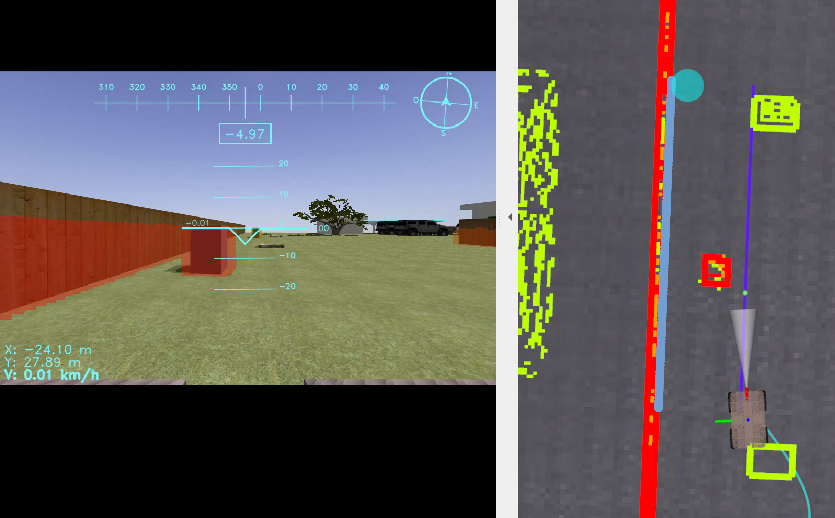
\includegraphics[width=\textwidth]{Corps_rapport/suivi_lisiere_05.png}        
    \end{subfigure}
    \hfill
    \begin{subfigure}[b]{0.25\textwidth}
        \centering
        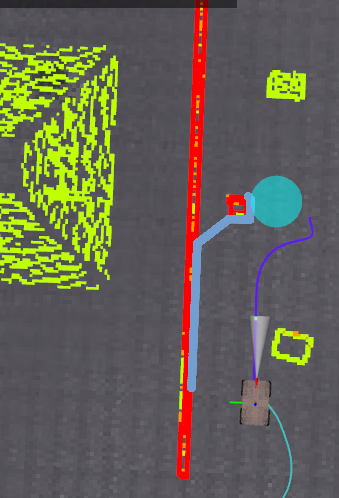
\includegraphics[width=\textwidth]{Corps_rapport/suivi_lisiere_1.png}
    \end{subfigure}
    \caption{Evaluation de la taille du cercle de détection de lisière sur la capacité à détecter la continuité de la lisière derrière un obstacle}
    \label{fig48}
\end{figure}

\indent L'idée suivante était de garder un petit cercle et d'introduire un mécanisme de mise à jour intelligent du chemin de suivi. Au début de mon stage, ce chemin était actualisé à chaque nouvelle détection de lisière, ce qui posait des problèmes lors des manœuvres de contournement d'obstacle car un nouveau chemin était calculé à partir de la lisière détectée sur l'obstacle lors de la manœuvre. L'objectif était donc de mettre à jour le chemin courant si et seulement si le nouveau chemin issu de la nouvelle détection de lisière est cohérent. Par cohérent, nous entendons un test de longueur de chemin car la longueur d'une lisière suivie ne baisse pas drastiquement entre deux déplacements élémentaires successifs du robot.\\

\indent Face aux limites des ajustements purement géométriques, l'approche retenue a consisté à conserver un rayon de détection restreint (garantissant un bon pouvoir de résolution) tout en introduisant un mécanisme de filtrage et de mise à jour dynamique cohérent du chemin de suivi. Initialement, le chemin de référence du robot était recalculé et écrasé de manière asynchrone à chaque nouvelle détection de lisière. Lors des phases de contournement, ce comportement générait des instabilités critiques : l'algorithme interprétait l'obstacle lui-même comme la nouvelle lisière à suivre, perturbant ainsi la trajectoire globale du robot.\\

\indent Pour résoudre ce problème, une logique de transition d'état conditionnelle a été implémentée. Désormais, le chemin courant n'est mis à jour par une nouvelle détection que si cette dernière respecte un critère de cohérence spatio-temporelle. Ce filtre repose sur l'hypothèse physique selon laquelle la longueur d'une lisière continue ne peut subir de variation drastique (diminution brutale) entre deux pas de calcul successifs du système (de l'ordre de quelques millisecondes). Mathématiquement, soit $L_{t}$ la longueur du chemin issu de la détection à l'instant $t$, et $L_{t-1}$ la longueur du chemin précédemment validé. La mise à jour du chemin de navigation est autorisée si et seulement si la longueur du nouveau chemin respecte l'équation suivante \eqref{eq8}:

\begin{equation}
\frac{L_{t-1}}{2} \leq L_{t}
\label{eq8}
\end{equation}

\begin{itemize}
\renewcommand{\labelitemi}{$\bullet$}
    \item \textbf{En cas de détection cohérente} : Si la condition est respectée, le chemin est mis à jour, garantissant l'adaptation du robot aux légères courbures de la lisière.
    \item \textbf{En cas d'anomalie ou de masquage} : Si la condition n'est pas respectée, la mise à jour est inhibée. Le robot conserve et suit son chemin précédent, ce qui lui permet de franchir la zone de perturbation (l'obstacle).\\
\end{itemize}

Malgré plusieurs ajustements fins (\textit{fine-tuning}) des paramètres du planificateur local et du contrôleur \textit{Pure Pursuit} — notamment l'augmentation de l'horizon de planification, la réduction du coût de rotation autour de l'axe $z$ pour le planificateur et l'accroissement de la distance de visée (\textit{lookahead distance}) du contrôleur —, le robot ne parvenait pas à contourner les obstacles présents sur la trajectoire de suivi. Il a été conclu que le contrôleur \textit{Pure Pursuit} n'offrait pas une liberté suffisante au planificateur local de type DWA (\textit{Dynamic Window Approach}). Ce dernier, agissant dans l'espace des commandes, ne pouvait pas modifier suffisamment les consignes de vitesse pour écarter le robot des obstacles. Une solution efficace consistait donc à déformer le chemin généré par l'algorithme de détection de lisière en amont du contrôleur \textit{Pure Pursuit}.\\

À cette fin, nous avons choisi d'implémenter un premier planificateur local dans l'espace de la tâche. Ce module prend en entrée le chemin issu de la détection de lisière ainsi que le nuage de points obstacles au tour du robot. Il génère une nouvelle trajectoire qui garantit le suivi de la lisière à la distance souhaitée tout en évitant les obstacles. Ce nouveau chemin est ensuite transmis au contrôleur \textit{Pure Pursuit}, dont les commandes de vitesse (linéaire et angulaire) sont vérifiées puis ajustées, si nécessaire, par le second planificateur local de type DWA avant d'être envoyées au robot.(\hyperref[fig49]{Figure 49})\\

Après concertation avec mon tuteur et d'autres membres de l'équipe, l'algorithme \textit{Elastic Band} (bandes élastiques) \cite{eband} a été choisi pour réaliser ce planificateur dans l'espace de la tâche.\\

\begin{center}
    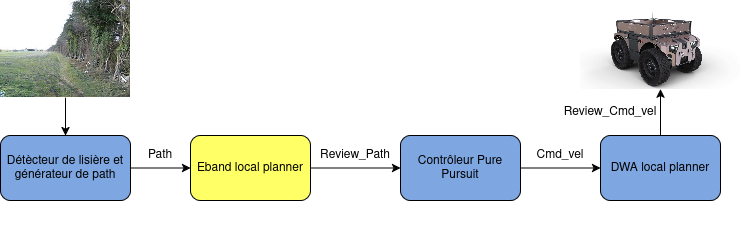
\includegraphics[width=1.0\linewidth]{Corps_rapport/org_review_border_follow.png}
    \captionof{figure}{Flowchart du mode de suivi de lisière revu}
    \label{fig49}
\end{center}

Dans la figure ci-dessus, sont représentés en bleu les modules déjà existants dans la stack MOBITER et en jaune le module à rajouter.

\paragraph{Fonctionnement du planificateur Elastic Band}

L'approche par \textbf{bandes élastiques} articule la planification globale et le contrôle réactif en temps réel en modélisant une trajectoire initiale sans collision sous la forme d'une structure flexible soumise à des forces virtuelles. En s'ajustant dynamiquement aux flux de données capteurs, la bande se déforme pour générer un parcours fluide et sécurisé face aux obstacles fixes ou mobiles, tout en minimisant localement sa longueur et en conservant la topologie du chemin d'origine. L'intérêt majeur de cette méthode réside dans son optimisation incrémentale : la qualité de la trajectoire s'affine continuellement à mesure que le robot progresse, tout en maintenant une charge de calcul minimale à chaque itération.\\

L’approche des bandes élastiques telle que proposée à l'origine se compose principalement de deux étapes : 

\begin{itemize}
\renewcommand{\labelitemi}{$\bullet$}
    \item \textbf{raffinement de la bande} : Cette étape consiste à supprimer les bulles inutiles et à combler les lacunes de la bande afin de réduire la charge de calcul.
    \item \textbf{optimisation de la bande} : Cette étape consiste à calculer les forces internes et externes et à modifier les positions des bulles en conséquence.
\end{itemize}


\subparagraph{a. Le concept des Bulles (Bubbles)}:

Pour fonctionner à des fréquences compatibles avec le contrôle temps réel ($\approx 10\text{ Hz}$ à $100\text{ Hz}$), l'algorithme évite le calcul coûteux de l'espace de configuration libre ($C\text{-space}$) global. Il introduit la notion de bulle de liberté locale $B(b)$.\\

\begin{itemize}

    \item \textbf{Définition géométrique (cas holonome 2D)} : Pour une configuration $b$, si $p(b)$ représente la distance minimale absolue entre le robot et l'obstacle le plus proche, la bulle $B(b)$ est définie par le disque centré sur $b$ et de rayon $q$ tel que:
    
    \begin{equation}
        B(b) = \{q : \Vert{}b - q\Vert{} < p(b)\}  
        \label{eq9}
    \end{equation}

    Tout point situé à l'intérieur de cette bulle garantit l'absence de collision avec l'environnement. \\

    \item \textbf{Extension aux robots orientables (3 DDL : $x, y, \theta$)} : La métrique de distance intègre la rotation via le rayon maximal $r_{\max}$ de la géométrie du robot par rapport à son centre :
    
    \begin{equation}
        D(\Delta b) = \sqrt{\Delta b_x^2 + \Delta b_y^2} + r_{\max} \vert{}\Delta b_\theta\vert{}
        \label{eq10}
    \end{equation}

    La bulle 3D s'exprime alors comme $B(b) = \{q : D(b - q) < p(b)\}$. \\

    \item \textbf{Condition de continuité de la bande} : La bande élastique est constituée d'une chaîne discrète de postures (via-points) associées à leurs bulles respectives. Pour garantir l'existence d'une trajectoire continue sans collision, deux bulles consécutives $B(b_i)$ et $B(b_{i+1})$ doivent obligatoirement se chevaucher ($\text{Overlap} \neq \emptyset$).\\

    \item \textbf{Adaptabilité spatiale} : La densité de discrétisation varie automatiquement. En zone dégagée, les bulles sont grandes et espacées, tandis qu'à proximité des obstacles, les bulles rétrécissent, augmentant la résolution locale du chemin.

\end{itemize}


\subparagraph{b. Modélisation de la déformation par forces artificielles}:

La forme du chemin est régie par un système de forces artificielles appliquées à chaque bulle $b_i$, cherchant un état d'équilibre quasi-statique. \\

\begin{itemize}

    \item \textbf{Force totale ($f$)} : La force totale appliquée à la bulle $b_i$ est la somme vectorielle des forces internes de contraction et des forces externes de répulsion :
    
    \begin{equation}
        f = f_c + f_r
        \label{eq11}
    \end{equation}

    \item \textbf{Force interne de contraction ($f_c$)} : Elle simule la tension mécanique d'un élastique pour raccourcir le chemin et supprimer le mou (slack) provoqué par les contours inutiles :
    
    \begin{equation}
        f_c = k_c \left( \frac{b_{i-1} - b_i}{\Vert{}b_{i-1} - b_i\Vert{}} + \frac{b_{i+1} - b_i}{\Vert{}b_{i+1} - b_i\Vert{}} \right)
        \label{eq12}
    \end{equation}

    où $k_c$ est le gain de tension interne. Les forces sont normalisées pour maintenir une tension uniforme le long de la chaîne. \\

    \item \textbf{Force externe de répulsion ($f_r$)} : Elle repousse la bande hors des zones à haut risque pour maximiser la marge de sécurité autour des obstacles :
    
    \begin{equation}
        f_r = \begin{cases}  k_r (\rho_0 - p) \dfrac{\partial p}{\partial b} & \text{si } p < \rho_0 \\  0 & \text{si } p \ge \rho_0  \end{cases}
        \label{eq13}
    \end{equation}    
    
    où $k_r$ est le gain de répulsion et $\rho_0$ représente le rayon d'influence de l'obstacle. Le gradient $\frac{\partial p}{\partial b}$ est estimé par différences finies locales. \\

    \item \textbf{Force modifiée et stabilité ($f^*$)} : Afin d'éviter le glissement longitudinal indésirable des bulles le long de la bande (ce qui provoquerait des cycles infinis de création/suppression de points), la force totale subie par une bulle est projetée sur l'axe orthogonal à la trajectoire :
    
    \begin{equation}
        f^* = f - \frac{f \cdot (b_{i-1} - b_{i+1})}{\Vert{}b_{i-1} - b_{i+1}\Vert{}^2} (b_{i-1} - b_{i+1})
        \label{eq14}
    \end{equation}

\end{itemize}

Lors du déplacement du robot ou des obstacles, la bande ajuste sa structure topologique par ré-échantillonnage :  \\
\begin{itemize}
\renewcommand{\labelitemi}{$\rightarrow$}
    \item Insertion de bulles : Si l'écartement entre deux bulles adjacentes devient trop grand au point de rompre leur chevauchement, une nouvelle bulle est insérée au milieu pour restaurer l'intégrité topologique du chemin. Si l'insertion échoue à rétablir le recouvrement, le déplacement est invalidé (signal d'échec nécessitant une re-planification globale).  
    \item Suppression de bulles : Si la bulle $B(b_i)$ devient redondante (i.e. si ses deux voisines $B(b_{i-1})$ et $B(b_{i+1})$ se chevauchent directement), la bulle $B(b_i)$ est supprimée pour alléger la charge de calcul.\\
\end{itemize}

 
\begin{comment}
Garantit la continuité $C^1$ de la trajectoire (ex. via splines sous contrainte de bulles), éliminant les arrêts aux angles morts. 
Calcul local basé uniquement sur la distance à l'obstacle le plus proche $p(b)$, dispensant de construire la map $C\text{-space}$ globale.  
Absorbe les bruits de perception et les obstacles imprévus en déformant la trajectoire sans recalculer un plan complet.  
La chaîne de bulles fournit une preuve géométrique formelle que la trajectoire déformée reste strictement sans collision.
\end{comment}

La trajectoire locale modifiée qui en résulte est ensuite transmise à un suiveur de trajectoire local qui calcule le point d’intersection entre la séquence de lignes reliant les centres des bulles et la circonférence de la bulle autour du robot. Le suiveur de trajectoire fait varier la vitesse en fonction de la taille des bulles et calcule enfin une vitesse sûre en tenant compte des limites de vitesse du robot et des bulles suivantes.


\paragraph{Résultats de l'implémentateur de  l'Elastic Band sur le mode de suivi de lisière}

Une fois le rajout de l'algorithme de bandes élastiques implémenté \cite{eband_planner} dans la stack, la modification du chemin de suivi de lisière a été testée en simulation. Les résultats ont montré que le robot était désormais capable de contourner les obstacles présents sur la trajectoire de suivi à condition que ces obstacles ne se trouvent pas directement sur le chemin de suivi car ceci résulte en un échec de l'optimiseur de l'algorithme de bandes élastiques qui se retrouve coincé dans un minimum local. La \hyperref[fig50]{Figure 50} suivante illustre bien cet echec : \\

\begin{figure}[H]
    \centering
    \begin{subfigure}[b]{0.325\textwidth}
        \centering
        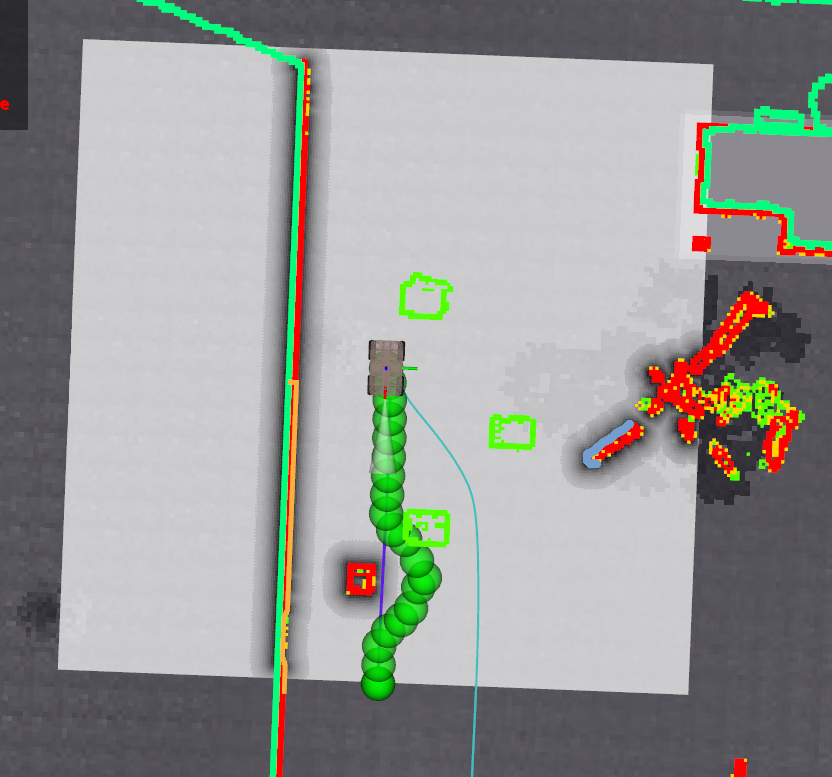
\includegraphics[width=\textwidth]{Corps_rapport/eband_3.png}   
        \caption{Contournement réussi d'un obstacle proche du chemin de suivi sans compression des bulles}
        \label{fig:image1}
    \end{subfigure}
    \hfill
    \begin{subfigure}[b]{0.325\textwidth}
        \centering
        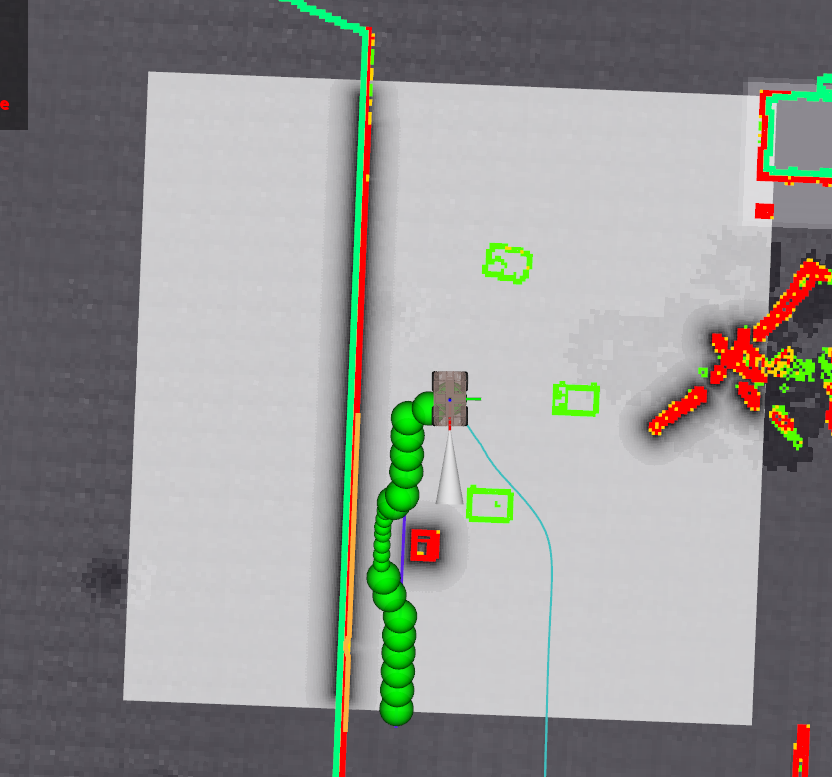
\includegraphics[width=\textwidth]{Corps_rapport/eband_2.png}
        \caption{Contournement réussi d'un obstacle proche du chemin de suivi avec compression des bulles}
        \label{fig:image2}
    \end{subfigure}
    \hfill
    \begin{subfigure}[b]{0.325\textwidth}
        \centering
        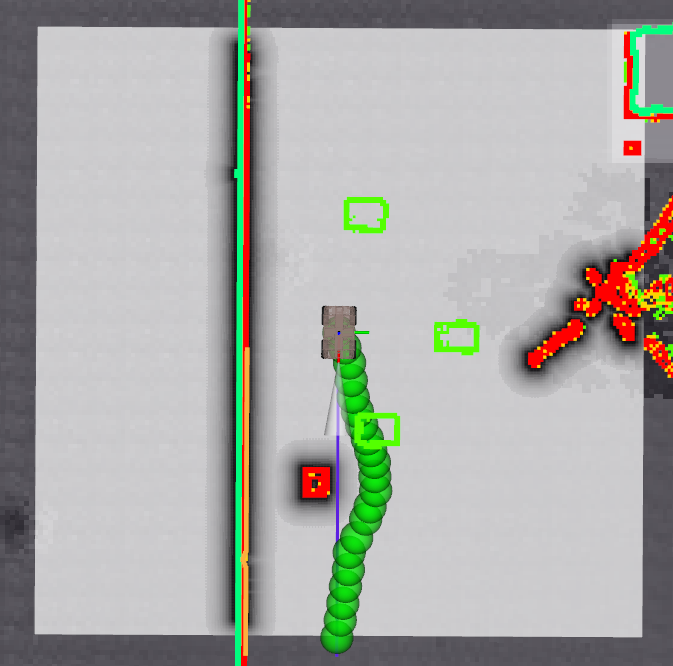
\includegraphics[width=\textwidth]{Corps_rapport/eband_1.png}
        \caption{Échec du contournement d'un obstacle placé directement sur le chemin de suivi}
        \label{fig:image3}
    \end{subfigure}
    \caption{Résultats de l'implémentation de l'algorithme original de bandes élastiques sur le suivi de lisière}
    \label{fig50}
\end{figure}

La \hyperref[fig:image3]{Figure 50(c)} illustre un échec de contournement lorsque l'obstacle est placé directement sur le chemin de suivi. Ce ci est logique car l'optimiseur de l'algorithme de bandes élastiques se retrouve coincé dans un minimum local. En effet, d'apres l'equation \eqref{eq13}, la gradient $\frac{\partial p}{\partial b}$ est nul lorsque le point representatif du robot se trouve sur l'obstacle et $p$ devient nulle, ce qui empêche l'optimiseur de se déplacer vers une position plus sûre car aucune force répulsive n'est générée.\\

La \hyperref[fig:image3]{Figure 50(c)} illustre un échec de contournement lorsque l'obstacle est placé directement sur le chemin de suivi. Ce comportement s'explique par le fait que l'optimiseur de l'algorithme des bandes élastiques se retrouve coincé dans un minimum local. En effet, d'après l'équation \eqref{eq13}, le gradient $\frac{\partial p}{\partial b}$ s'annule lorsque le point représentatif du robot se situe exactement sur l'obstacle et que la distance $p$ devient nulle. Cela empêche l'optimiseur de dévier la trajectoire vers une position plus sûre, aucune force répulsive n'étant alors générée.\\



\paragraph{Modification de l'optimiseur de l'algorithme de bandes élastiques}





















\begin{comment}

\subsubsection{Intégration des dernières modifications de la brique de cartographie après refactoring}
Une fois le projet bien pris en main, une première mission m'a été confiée pour, d'une part, me familiariser avec la méthodologie de versionnement sur Git et, d'autre part, prendre en main la procédure de mise en route du robot et de la Brique MOBILEX*.\\\\
Le projet venait de subir une refonte complète et la brique de cartographie, qui avait été modifiée sur l'ancienne version afin d'ajouter un filtre de Kalman* permettant de pondérer la mise à jour de la carte en fonction de la confiance accordée aux données provenant des capteurs, devait être intégrée à la nouvelle version de la Brique MOBILEX* puis testée. Cette intégration consistait à revoir le mapping des topics et le nom des paquets appelés, ainsi qu'à ajouter l'installation des nouvelles librairies dans la procédure d'installation du projet et leur appel dans les paquets en modifiant les fichiers CMakeLists utilisés pour la compilation* de ces derniers.\\\\
Après avoir intégré et testé en simulation le bon fonctionnement de cette dernière, M. Barbier et moi sommes allés la tester à l'INRAE. Le robot n'ayant pas été réutilisé depuis la refonte du projet, il a fallu, dans un premier temps, remettre l'installation au propre. J'ai ensuite pu me familiariser avec la procédure de mise en route du projet sur le robot.\\\\
Pour tester la brique, nous avons lancé la Brique MOBILEX* complète incluant cette dernière dans des conditions idéales, c'est-à-dire avec une position précise au centimètre fournie par le GNSS RTK. Pour obtenir cette précision, une base fixe dont la position est connue de manière précise compare la position calculée à partir du signal GPS avec sa vraie position et envoie des corrections au récepteur présent sur le robot. Il a alors suffi de couper l'envoi des corrections pour dégrader volontairement la précision de la position afin de s'assurer que la carte ne se dégrade pas trop rapidement.\\\\
Les résultats ont montré que la carte se mettait moins à jour, ce que nous souhaitions, mais que les mesures imprécises restaient tout de même trop prises en compte, rendant la carte inexploitable au bout de quelques secondes (\hyperref[fig20]{Figure 20} et \hyperref[fig21]{21}).\\
\begin{center}
    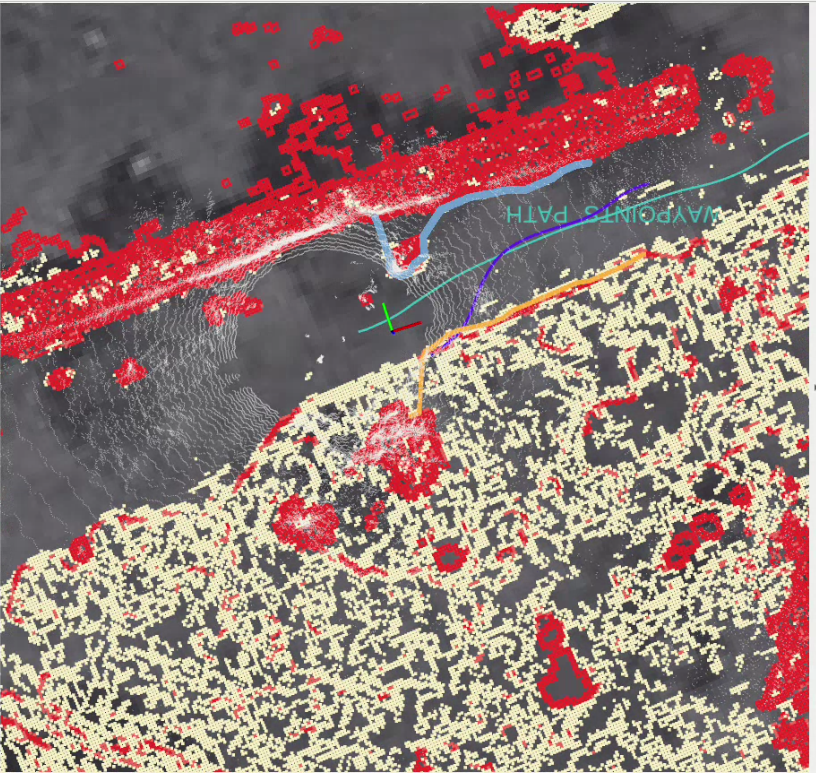
\includegraphics[width=0.7\linewidth]{Corps_rapport/map_rtk.png}
    \captionof{figure}{Carte des obstacles avec GNSS RTK}
    \label{fig20}
\end{center}
\begin{center}
    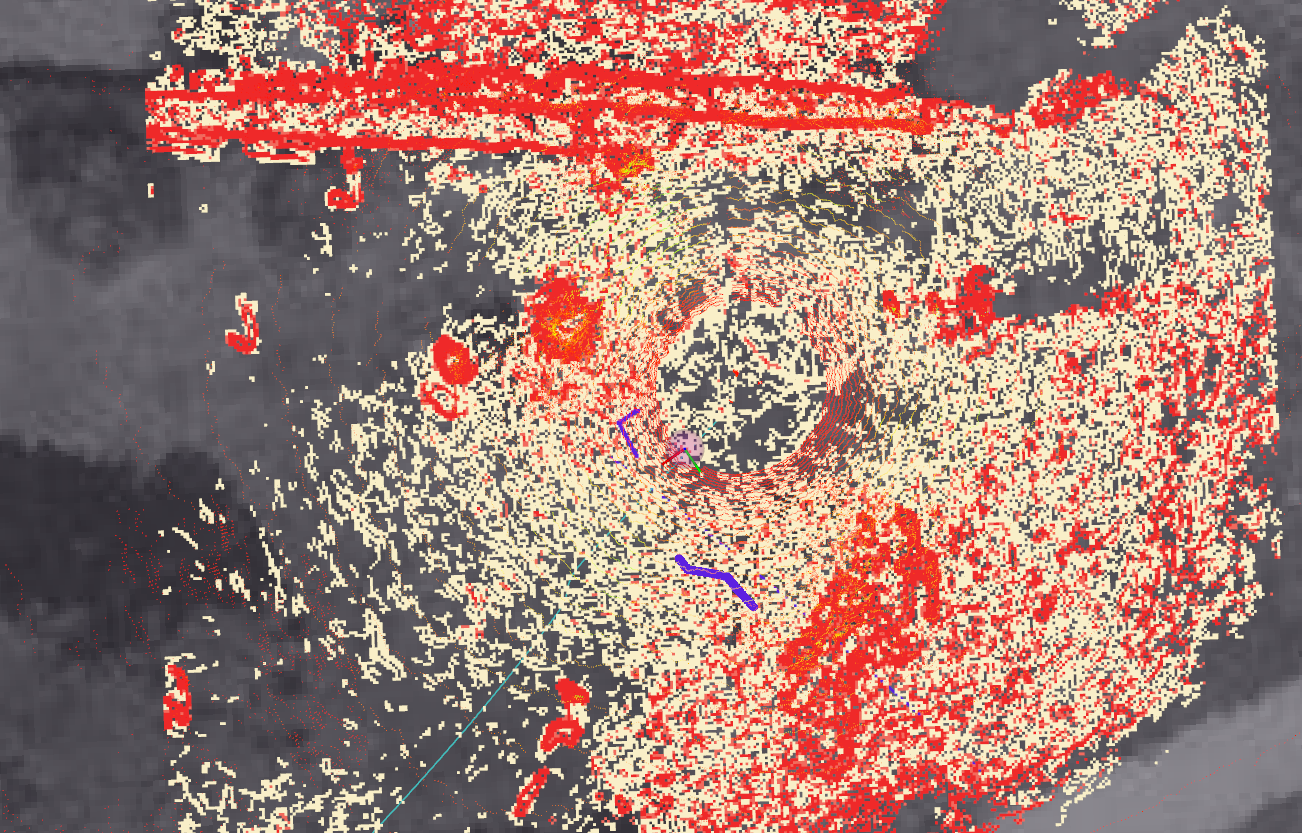
\includegraphics[width=1\linewidth]{Corps_rapport/map_sans_rtk.png}
    \captionof{figure}{Carte des obstacles après 5 secondes de perte des corrections du mode RTK}
    \label{fig21}
\end{center}

Une solution simple a alors été envisagée. Elle consiste à détecter toute anomalie sur le fonctionnement du GNSS en mode RTK pour ajouter un switch visant à sous-estimer la précision de la position retournée dès lors que la fiabilité de la mesure n'est plus garantie (problème de capteur, d'envoi des corrections, de couverture GPS, etc.).\\\\
Pour préparer l'ajout de ce switch, il m'a été demandé d'ajouter une fonction Python permettant de vérifier tout un ensemble de paramètres à tout instant et de publier le résultat de la vérification sous la forme d'un flag.
\subsubsection{Investigations sur un problème de téléopération}
Lors des tests à l'INRAE, la présence d'une personne de l'institut est obligatoire et un ingénieur a été recruté l'an dernier pour encadrer ces tests.\\\\
Lors des tests de la nouvelle brique de cartographie, cette personne a constaté que le robot mettait plus de temps à réagir en téléopération à plus de $2\ m.s^{-1}$ qu'avant le refactoring, que lors de tests réalisés par l'INRAE avec leur propre brique de commande ou qu'en le contrôlant avec la télécommande fournie par SHARK Robotics.\\\\
La téléopération assistée devait être présentée à la DGA lors de la revue d'avancement prévue le mois suivant. M. Barbier et moi avons alors investigué sur ce problème en urgence.\\\\
La première piste explorée fut un délai potentiel au sein de la chaîne de commande. En remontant l'ensemble de la chaîne de commande, nous n'avons pas trouvé de délai entre la réalisation d'une commande à la manette et sa traduction en vitesses de roues à envoyer au robot. Cependant, en comparant les instants d'envois des commandes au robot et le moment où le robot réagissait à ces dernières, on observait un décalage de l'ordre de $0,5\ s$.\\\\
L'hypothèse alors formulée était que notre interface du robot programmée en Python faisait appel à des fonctions de communication provoquant ce délai de $0,5$ seconde, là où l'INRAE utilisait une interface en C++ faisant appel à d'autres fonctions pour communiquer avec le robot ne provoquant pas ce délai. Le problème était que les tests réalisés par l'INRAE remontaient à longtemps et qu'ils n'arrivaient pas à remettre en route leurs codes, mais nous ont dit que leur interface était une adaptation de notre interface pour l'intégrer à leur environnement.\\\\
Nous avons alors décidé de récupérer leur interface pour pouvoir la comparer avec la nôtre et l'intégrer dans notre Brique MOBILEX* pour avoir une interface en C++. Cette réintégration n'a rien changé sur le comportement du robot.\\\\
En examinant la réponse du robot à l'envoi d'une commande en téléopération, je me suis rendu compte qu'en plus du délai de $0,5$ seconde observé, il y avait des dépassements de l'ordre de 30 \% sur la vitesse angulaire, pouvant causer ces difficultés de contrôle.\\\\
J'ai alors proposé de refaire le paramétrage du correcteur de taux de lacet.\\\\
N'ayant pas de modèle du système, nous avons réalisé ce paramétrage à la main comme il est courant de faire pour un correcteur PID. Pour éviter de trop abîmer le terrain, nous avons utilisé des consignes échelons faibles de $0,25\ rad.s^{-1}$.\\\\
En vérifiant le bon fonctionnement du correcteur lors d'un suivi de waypoints, nous nous sommes rendu compte que le modèle que nous cherchions à asservir n'est pas linéaire car là où il n'y avait aucune anomalie notable à $0,25\ rad.s^{-1}$, on observait des dépassements de 20 \% à $2\ rad.s^{-1}$.\\\\
Il a alors été proposé de réaliser une linéarisation par partie du correcteur pour atténuer ces phénomènes, mais que cette solution serait étudiée ultérieurement car elle n'interviendrait pas dans l'urgence actuelle de résoudre les problèmes de téléopération avant la revue d'avancement prévue deux semaines plus tard.\\\\
En inspectant les commandes angulaires fournies par le nœud Joy\_node, nous nous sommes rendu compte que le joystick analogique avait une grande zone morte, faisant passer le joystick de la position nulle à maximale au plus petit mouvement. De plus, les échelles de consignes de vitesse angulaires étaient de $0$ à $3\ rad.s^{-1}$ là où l'INRAE allait de $0$ à $1\ rad.s^{-1}$. L'achat d'un joystick de meilleure qualité et la modification de l'échelle ont permis de grandement améliorer le contrôle du robot lors de virages, mais il restait lent à s'arrêter en comparaison avec le contrôle à la manette fournie par SHARK Robotics.\\\\
La configuration des pentes d'accélération et de décélération dans l'interface du Barakuda a alors été remise en question car l'ancien ingénieur de SHERPA Engineering qui avait travaillé sur l'interface n'avait pas documenté le choix de la limite d'accélération à $1.38\ m.s^{-2}$. Il se trouve que cette valeur avait été donnée à l'oral par un ingénieur de SHARK Robotics pour protéger les variateurs du robot. Cependant, en mesurant les accélérations réalisées par la télécommande du robot, on s'est rendu compte que les limites d'accélérations utilisées sont supérieures à $2.5\ m.s^{-2}$ et que la décélération est encore plus franche car le robot serre ses freins lors du relâchement du joystick.\\\\
Lors d'une réunion organisée par la DGA regroupant l'ensemble des consortiums et des représentants de SHARK Robotics, nous avons posé la question de la nécessité de limiter l'accélération du robot à $1.38\ m.s^{-2}$ alors que la télécommande fournie ne l'est pas, et il se trouve qu'aucun autre consortium n'avait reçu cette indication et les représentants de SHARK Robotics n'étaient pas non plus au courant de cette limitation. Nous avons alors décidé d'aligner nos rampes d'accélérations sur celles de la télécommande du robot, soit $2.5\ m.s^{-2}$, ce qui a résolu le problème de contrôle en téléopération et permis au passage de diminuer le temps de prédiction des LUTs de la planification locale, la rendant plus permissive.
\subsubsection{Installation et test de la sémantique caméra}
Une fois l'urgence résolue, nous avons pu reprendre les tests des ajouts pour le défi 2. Un des grands enjeux du défi 2 à traiter est la présence d'herbes hautes, de fumée et de brouillard parasitant le LIDAR*. \\\\
La solution imaginée pour répondre à cette problématique est l'utilisation de la sémantique caméra.\\\\
La brique de sémantique caméra a alors été développée pour évaluer dans un premier temps la faisabilité de la solution.\\\\
M. Barbier et moi nous sommes alors occupés d'installer l'ensemble des outils utilisés par cette nouvelle brique sur le robot et avons évalué ses performances lors de la détection du sol et de la fumée.\\\\
L'évaluation des performances consistait à vérifier la qualité de la détection du sol, y compris dans les herbes hautes, et de la fumée lorsque le robot est à l'extérieur et à l'intérieur de cette dernière, le tout en s'assurant que la charge CPU et GPU induite par la segmentation* ne compromette pas les performances temps-réel de la Brique MOBILEX*.\\\\
Les résultats obtenus montrent que la segmentation* fonctionne globalement bien pour la détection du sol (\hyperref[fig22]{Figure 22}) malgré certaines frames où le détecteur open-set ne détecte rien, et que les performances temps-réel sont toujours assurées (temps d'inférence* ~60 ms). Cependant, la détection de la fumée n'est quant à elle pas exploitable en l'état. Lorsque le robot est à l'extérieur de la fumée, il ne détecte qu'une partie de cette dernière (\hyperref[fig23]{Figure 23}) et lorsqu'il se situe dans la fumée, le détecteur open-set ne détecte plus rien (\hyperref[fig24]{Figure 24}).\\
\begin{center}
    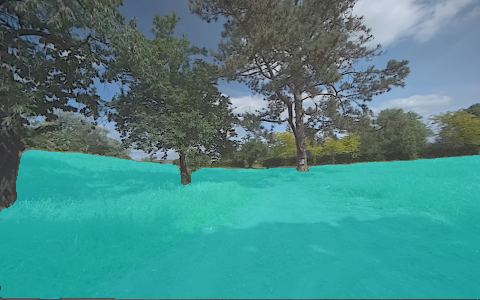
\includegraphics[width=0.8\linewidth]{Corps_rapport/ground.png}
    \captionof{figure}{Segmentation du sol}
    \label{fig22}
\end{center}
\begin{center}
    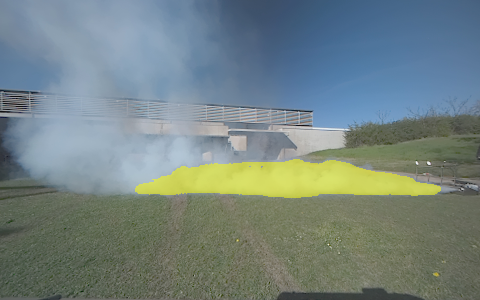
\includegraphics[width=0.8\linewidth]{Corps_rapport/fumee_exterieur.png}
    \captionof{figure}{Segmentation de la fumée depuis l'extérieur}
    \label{fig23}
\end{center}
\begin{center}
    
\includegraphics[width=0.8\linewidth]{Corps_rapport/fumee.png}
    \captionof{figure}{Segmentation de la fumée au sein de cette dernière}
    \label{fig24}
\end{center}
\subsubsection{Calibration extrinsèque caméra-LIDAR}
La phase d'évaluation étant concluante pour la détection du sol, l'utilisation de la sémantique caméra a été retenue pour pouvoir naviguer dans les hautes herbes.\\\\
Pour pouvoir intégrer cette solution au projet, il a été nécessaire de réaliser la calibration extrinsèque entre la caméra et le LIDAR*, car ces derniers seront voués à être fusionnés lors de la création de la carte. Plus précisément, la solution planifiée serait de se servir du nuage de points produit par la ZED pour d'une part avoir une redondance capteur pour diminuer le manque d'information dans la carte à l'avant du véhicule et anticiper la gestion des pannes capteurs et d'autre part, fournir une information sémantique dans les différentes tuiles de la carte.\\\\
Étant devenu familier avec la procédure d'utilisation du robot, cette tâche m'a été confiée en toute autonomie.\\\\
La première idée de calibration était de réaliser la calibration à tâtons en projetant le nuage de points LIDAR* dans l'image caméra et de modifier la transformation entre la caméra et le LIDAR* jusqu'à ce que les points se superposent correctement dans une scène contenant des objets de différentes tailles à différentes distances.\\\\
Lors des tests de visualisation de la superposition du nuage de points de la caméra avec celui du LIDAR*, les résultats n'étaient pas concluants, ce qui nous a laissé penser que la calibration réalisée n'était pas suffisamment précise.\\\\
Une calibration plus qualitative a alors été imaginée en réalisant une méthode ICP point-to-plane entre le nuage de points de la caméra et le nuage de points LIDAR*. La méthode ICP point-to-plane est une technique utilisée pour aligner deux nuages de points en trois dimensions. Contrairement à la méthode ICP point-to-point, qui minimise la distance entre les points correspondants des deux nuages, la méthode point-to-plane minimise la distance entre les points d'un nuage et les plans tangents estimés à partir de l'autre nuage de points.\\\\
Cette méthode est souvent préférée dans les applications où les nuages de points ont des densités différentes ou lorsque l'on souhaite obtenir une meilleure précision dans l'alignement, ce qui est notre cas, car le nuage de points de la caméra est bien plus dense que celui du LIDAR*.\\\\
Pour réaliser cette méthode ICP, j'ai commencé par créer un nœud ROS* me permettant d'extraire les nuages de points caméra et LIDAR* dans leur repère respectif et de les enregistrer dans des fichiers binaires. Ensuite, j'ai créé un script Python me permettant de lire le contenu de ses fichiers, de filtrer les points et, en me servant de la bibliothèque Open3D, de réaliser la méthode ICP en point à plan et de visualiser le résultat.\\\\
La calibration par la méthode ICP était sensiblement proche de la précédente et lors de la visualisation avec Open3D (\hyperref[fig25]{Figure 25}) les nuages de points se superposaient bien tandis que lors des tests, la visualisation sur RVIZ était toujours décalée (\hyperref[fig26]{Figure 26}).\\
\newpage
\begin{figure}[h]
    \centering
    \begin{subfigure}[b]{0.7\textwidth}
        \centering
        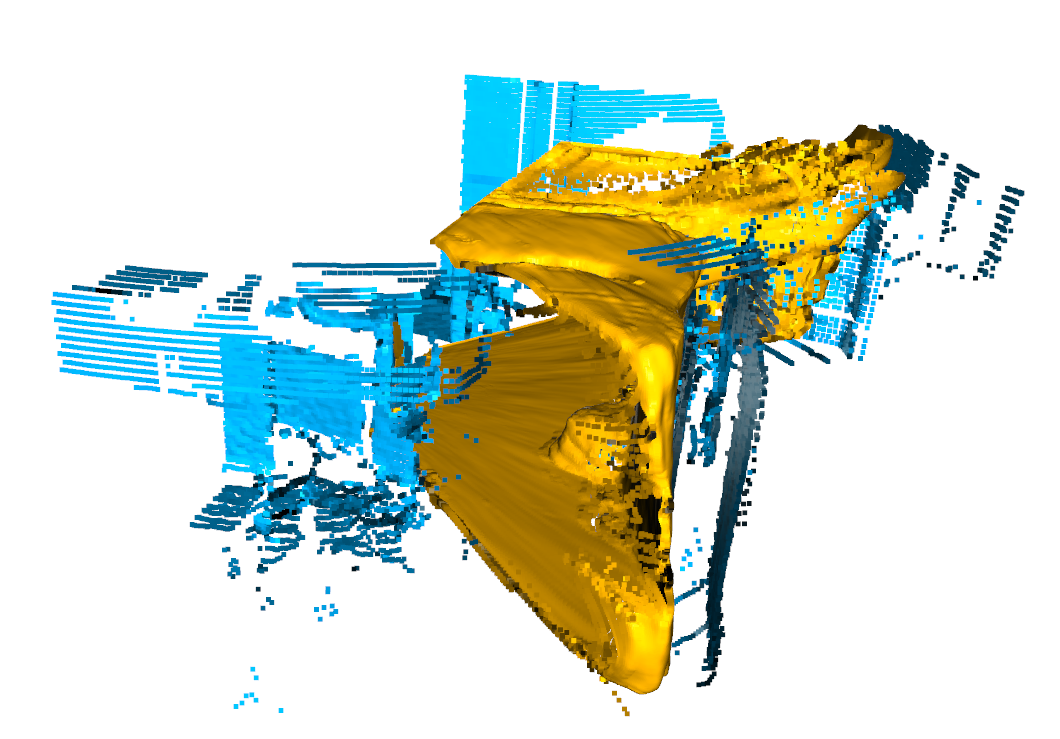
\includegraphics[width=\textwidth]{Corps_rapport/ICP_avant_tf.png}
        \caption{Avant transformation}
        \label{fig:image5}
    \end{subfigure}
    \begin{subfigure}[b]{0.7\textwidth}
        \centering
        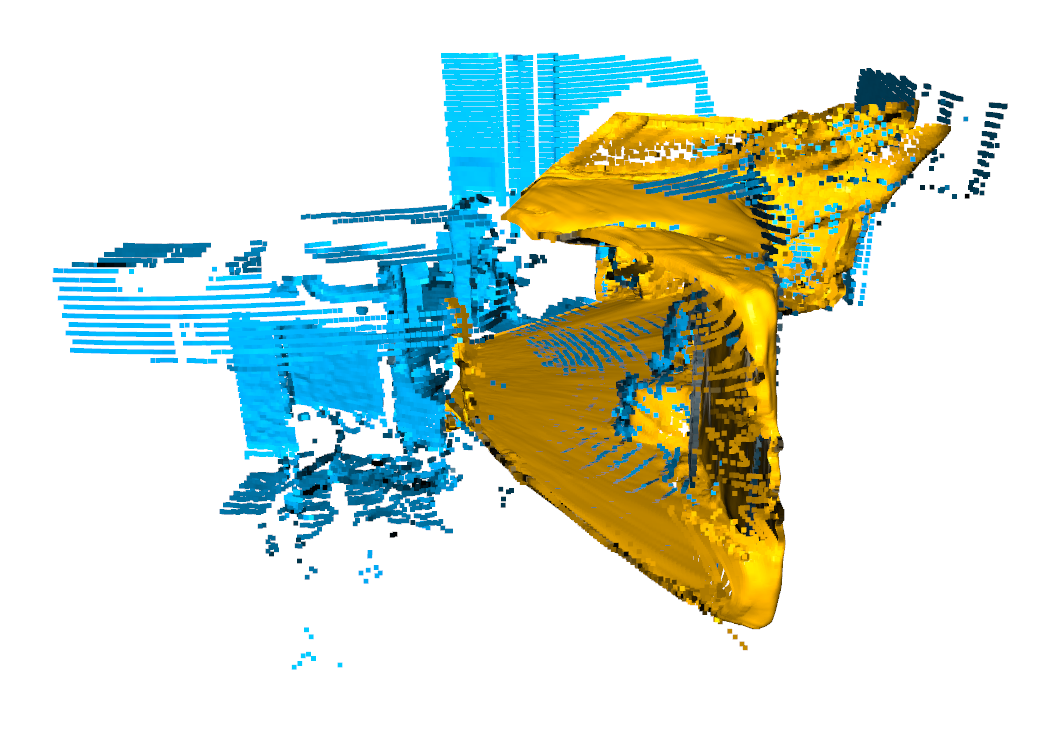
\includegraphics[width=\textwidth]{Corps_rapport/ICP_apres_tf.png}
        \caption{Après transformation}
        \label{fig:image6}
    \end{subfigure}
    \caption{Calibration extrinsèque Caméra-LIDAR par la méthode ICP point to plane}
    \label{fig25}
\end{figure}
\newpage
\begin{center}
    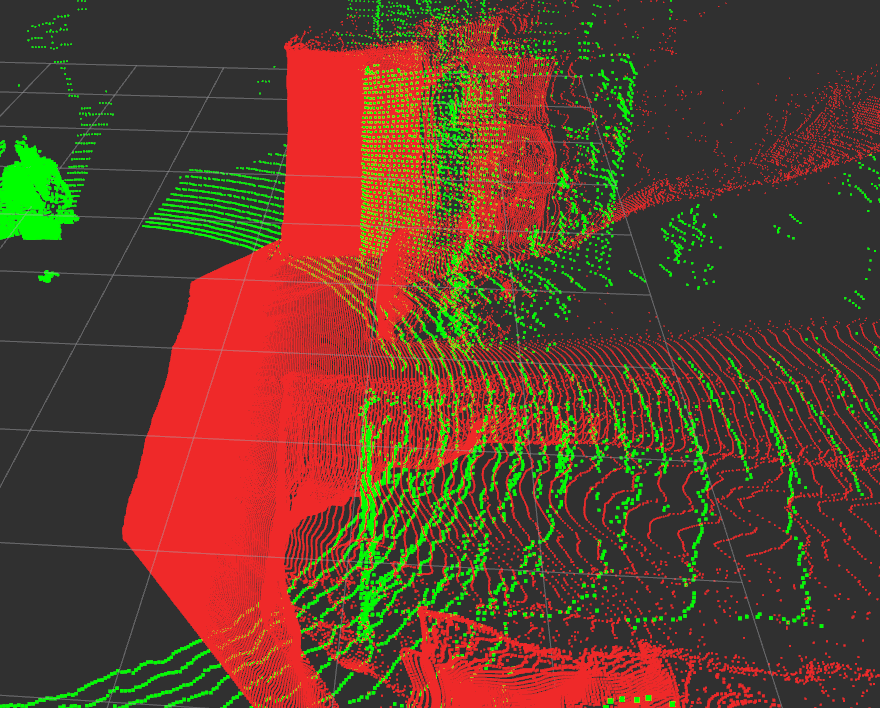
\includegraphics[width= 0.6\linewidth]{Corps_rapport/lidar_camera_mv_tf.png}
    \captionof{figure}{Visualisation de la calibration extrinsèque sous RVIZ}
    \label{fig26}
\end{center}
$\ $\\
Mes doutes se sont alors penchés sur une mauvaise publication de la transformation entre la caméra et le LIDAR* et après un peu d'inspection, je me suis rendu compte que le problème provenait du driver de la caméra qui écrasait continuellement notre transformation en la remplaçant par une transformation identité.\\\\
Après modification du fichier launch du driver, les nuages de points caméra et LIDAR* se superposent comme souhaité (\hyperref[fig27]{Figure 27}).\\
\begin{center}
    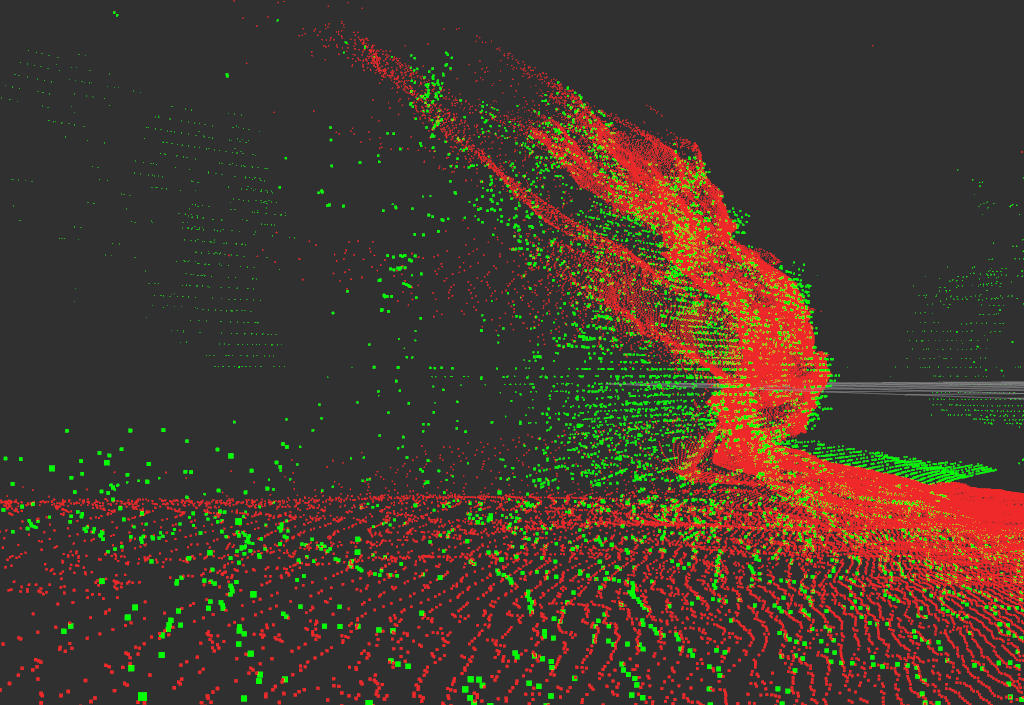
\includegraphics[width=0.8\linewidth]{Corps_rapport/lidar_camera1.png}
    \captionof{figure}{Visualisation de la calibration extrinsèque sous RVIZ après correction du driver}
    \label{fig27}
\end{center}
\subsubsection{Test du nouveau suivi de lisière}
Lors du premier défi, deux problèmes avaient été identifiés : un problème de détection de la lisière lors de la présence d'angles droits et un problème concernant la génération de la trajectoire du suivi de lisière avait été constaté. La trajectoire générée pouvait traverser le bas-côté à suivre. Ce problème était cependant masqué par la couche du local planner qui empêchait au robot d'entrer dans le bas-côté, ce qui faisait que le robot arrivait tout de même à suivre les lisières, mais anormalement lentement.\\\\
Cette génération de trajectoire a alors été modifiée en une translation de la lisière détectée selon la direction de la moyenne des normales de la détection tandis que le problème de détection dans les angles droits a été rectifié en ajustant les paramètres du détecteur.\\\\
Lors de mes tests de ces modifications, je me suis rendu compte que la lisière fluctuait d'une détection à l'autre, ce qui forçait le correcteur à diminuer sa vitesse pour tenter de s'aligner en permanence à la trajectoire donnée.\\\\
Pour pallier ce problème, j'ai pris l'initiative d'assouplir les contraintes du correcteur en augmentant la distance du point de visée anticipée et en diminuant l'impact du rayon de courbure de la trajectoire sur la vitesse linéaire. Cela nous donne un correcteur allant bien plus vite moyennant des écarts latéraux à la courbe un peu plus importants.\\\\
J'ai alors présenté mes résultats à l'équipe qui les a validés.
\subsubsection{Installation et configuration du réseau avec 2 interfaces}
 Historiquement, il n'y avait sur le robot et le PC débarqué que les antennes 5 GHz mais, lors des épreuves du premier défi, il y a eu des problèmes de communication lorsque le robot passait derrière des obstacles denses. \\\\
 Pour pallier ce problème, ces antennes ont d'abord été remplacées par des antennes 2,4 GHz sauf que la télécommande du robot utilise également ce type d'antennes, ce qui provoquait des perturbations et rendait le robot inutilisable. Un compromis a alors été imaginé en remettant les antennes 5 GHz pour faire passer les importants flux de données, majoritairement utilisés pour du débug, et en ajoutant des antennes 868 MHz pour assurer une communication fiable des données nécessaires au fonctionnement du robot, c'est-à-dire l'envoi des commandes et le retour vidéo pour le téléopérateur.\\\\
 L'ingénieur de tests INRAE et moi avons été chargés d'installer et de configurer les antennes 868 MHz. Un problème s'est rapidement posé, les antennes ne sont pas compatibles POE actif et ne pouvaient donc pas être installées sur les 4 ports POE du calculateur. Il restait alors 2 ports déjà utilisés : le premier par la carte électronique SHERPA et le second par l'antenne 5 GHz.\\\\
 J'ai alors pensé à une solution faisant intervenir un routeur pour pouvoir rediriger les données provenant du réseau 5 GHz et du réseau 868 MHz à l'interface réseau du robot. J'ai vu qu'il existait des switchs permettant de créer des VLANs et de faire du routage entre ces VLANs, ce qui aurait permis d'avoir les 2 réseaux sur un même switch et de faire le routage vers l'interface du réseau. Malheureusement, l'INRAE ne possédait qu'un switch ne proposant pas cette fonctionnalité.\\\\
Après quelques recherches, nous nous sommes rendu compte qu'il est possible de donner plusieurs adresses IP à une même interface réseau. En affectant une adresse pour chaque antenne à l'interface, nous avons pu configurer le réseau en n'utilisant qu'une interface du PC embarqué et un switch ordinaire.\\\\
On obtient alors l'architecture réseau \hyperref[fig28]{Figure 28} :
\begin{center}
    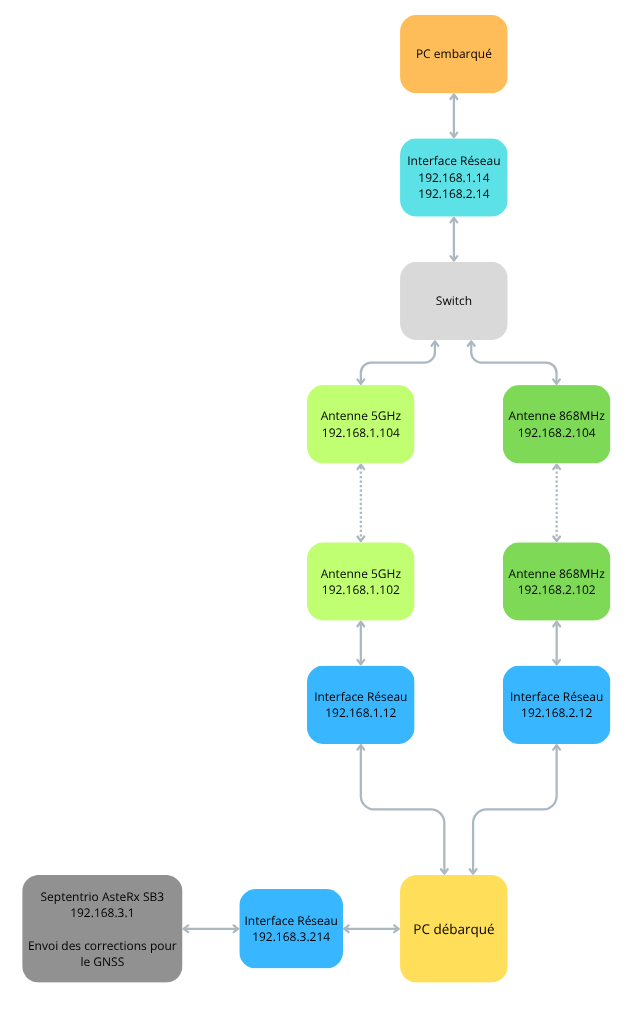
\includegraphics[width=0.7\linewidth]{Corps_rapport/PC débarqué.png}
    \captionof{figure}{Diagramme synoptique de l'architecture réseau du système}
    \label{fig28}
\end{center}
\subsubsection{Configuration et test de l'envoi d'images compressées sur l'antenne 868MHz}
L'installation double antenne étant fonctionnelle, il a alors fallu configurer le routage des différentes données sur les bonnes interfaces et automatiser à l'aide de scripts bash les opérations nécessaires au choix de l'interface à utiliser.\\\\
Une mesure de la bande passante des antennes 868 MHz a révélé que cette dernière était bien trop faible (150 ko/s) pour pouvoir transmettre l'image annotée au PC déporté. Une compression de cette dernière en h265 a alors été mise en place, divisant la bande passante nécessaire par plus de 200, la faisant passer de 17Mo/s à 80ko/s, pour une qualité à peine dégradée.\\\\
La compression h265 nécessite d'encoder l'image du côté du PC embarqué avant de l'envoyer au PC débarqué, ce qui nécessite un décodage du côté de ce dernier. \\\\
Des tests de fiabilité de la liaison ont alors été réalisés, pour comparer le réseau 5 GHz et le réseau 868 MHz, notamment sur la portée et la résilience lors de la présence d'obstacles (bâtiments et végétation dense) entre le PC débarqué et le robot.\\\\
Pour ces tests, l'envoi de l'image encodée a été fait sur chaque réseau en temps réel et le décodage a été réalisé par deux nœuds distincts. Nous avons alors pu afficher les deux retours vidéo côte à côte pour les comparer.\\\\
Les résultats obtenus montrent que l'ajout de la compression sur le retour vidéo a considérablement réduit les problèmes de communication de l'antenne 5 GHz, et que cette dernière était plus fiable, que ce soit en présence d'obstacles ou à grande distance. Nous avons alors conclu que l'ajout de l'antenne 868 MHz n'était pas nécessaire et que l'ajout de la compression ainsi qu'un choix sur les données à transmettre permettent de contrôler le robot à plus de 150 m en présence d'obstacles sans coupures, ce qui sera largement suffisant pour le défi 2.
\subsubsection{Autres tests réalisés}
D'autres tests ne rencontrant pas de problèmes particuliers ont été réalisés comme par exemple :\\
\begin{itemize}
    \item Une journée de tests à Montoldre pour tester l'ajout de la prise en compte du manque d'information dans la carte comme des obstacles au fur et à mesure que le robot s'en approche et pour évaluer les améliorations apportées par le refactoring sur la stabilité du robot lors de la conduite autonome à 3 m/s. Le seul problème noté ce jour-là était que le robot opérait de gros virages lors du retrait de l'arrêt d'urgence de sa télécommande pour lancer la conduite autonome de ce dernier. Le problème provenait du gain intégral qui commençait à s'accumuler dès lors que la conduite autonome était lancée par le téléopérateur, avant même d'avoir retiré l'arrêt d'urgence.\\
    \item Le test du mode safety first en téléopération qui ne présenta qu'un léger problème d'affichage dans l'IHM.\\
    \item Le test d'une nouvelle IHM, avec comme objectif d'évaluer l'amélioration de l'ergonomie pour qu'elle soit utilisable par une personne ne travaillant pas sur le projet. Quelques bugs mineurs ont été constatés dont un problème sur l'ajout de paramètres reconfigurables dynamiquement avec dynamic reconfigure. J'ai finalement réussi à résoudre le problème et ayant trouvé la fonctionnalité intéressante pour faciliter le paramétrage des correcteurs, j'ai modifié les briques contenant des correcteurs Pure Pursuit et longitudinaux ainsi que le correcteur de taux de lacet inclus dans l'interface du Barakuda pour ajouter la possibilité de modifier les gains dynamiquement.\\
    \item Une assistance lors des tests d'une nouvelle loi de commande avec observateurs de glissement développées par l'INRAE, qui a récemment été abandonnée car son utilisation n'était pas indispensable et que j'avais pointé une incohérence dans le protocole de tests qui était que l'on comparait pour une même trajectoire, l'écart du robot à cette dernière lors de l'utilisation de la loi de commande de l'INRAE et lors de l'utilisation du contrôleur Pure Pursuit et de la régulation longitudinale actuellement utilisés. Le problème était que la loi de commande INRAE ne fait aucune régulation de vitesse à l'approche de virages. Les résultats obtenus auraient donc été en faveur de la loi actuellement utilisée. L'utilisation de la loi de commande INRAE sera revue avec l'ajout d'une régulation longitudinale lorsque nous observerons une incontrôlabilité du robot à cause de glissements, peut-être lorsque nous monterons en vitesse.
\end{itemize}
\subsubsection{Intégration d'un planificateur global RRT*}
Enfin, en parallèle de mes tests, une tâche de fond m'a été proposée pour m'initier à la programmation en C++ lors des périodes de creux. Cette tâche consistait à reprendre un planificateur global RRT* réalisé par un ancien stagiaire l'an dernier sur la Brique MOBILEX* avant refactoring et de l'intégrer à la nouvelle version. Ce planificateur permettrait de s'affranchir de la contrainte de discrétisation du chemin liée à l'échantillonnage du MNE car les nœuds sont générés dans l'espace continu. \\\\
Le planificateur était une classe héritant d'autres classes qui avaient été modifiées lors du refactoring.\\\\
J'ai commencé par me former rapidement au concept de programmation orientée objet avec un cours d'OpenClassrooms puis j'ai pu intégrer cette classe en comparant le comportement du planificateur A* avant et après refactoring pour adapter le RRT* afin qu'il fonctionne avec les nouvelles méthodes utilisées.\\\\
Le RRT* fonctionne mais doit être modifié dans l'objectif de fournir des courbes C2, c'est-à-dire des courbes dont la dérivée seconde est continue.
\subsection{Travaux à venir}
Étant à peine plus de la moitié de mon stage, beaucoup de développements ont été réfléchis ou entamés, nécessitant des tests à venir.\\\\
En voici une liste non exhaustive :
\subsubsection{Tests de l'intégration de la détection et prise en compte des pentes et dévers}
Pour détecter et caractériser le caractère franchissable ou non des pentes et dévers, une solution consistant à se resservir du filtre de Sobel utilisé pour la détection des obstacles est envisagée, avec la particularité d'être utilisé sur une version sous-échantillonnée du MNE et avec de nouveaux seuils.\\\\
Les tests consisteront alors à s'assurer que le robot s'engage dans des pentes et dévers franchissables et contourne celles et ceux qui ne le sont pas.
\subsubsection{Tests de l'intégration de la couche sémantique dans le MNE}
Pour pouvoir intégrer les informations sémantiques dans le MNE, la solution retenue est d'attribuer à chaque point du nuage de points de la caméra une information de franchissabilité ou non. Ensuite, lors de la fusion du nuage de la caméra et du nuage LIDAR* pour mettre à jour la carte, cette information serait ajoutée aux tuiles de la carte, uniquement par les points du nuage de la caméra.\\\\
Les tests consisteront alors à vérifier que le robot puisse s'engager dans des herbes hautes.
\subsubsection{Tests de l'intégration de la couche ultrasonique dans le MNE}
Un point dur du défi 2 est la gestion des obstacles transparents car ces derniers ne sont ni détectés par le LIDAR*, ni détectés par la caméra. Une solution en cours d'évaluation serait d'utiliser les capteurs ultrasoniques pour les fusionner avec les nuages de points LIDAR* et caméra dans le MNE.\\\\
Des premiers tests ont été réalisés pour évaluer l'enveloppe de détection du capteur et la fiabilité des détections.\\\\
Les résultats obtenus montrent que le capteur pourrait nous permettre de détecter des obstacles d'au moins 50x50 cm jusqu'à 4 mètres, mais que l'orientation de ces derniers pourrait grandement affecter la distance à partir de laquelle ils seraient détectés.\\\\
Malgré ces résultats mitigés, cette solution a été retenue faute d'autres alternatives et d'autres tests seront à réaliser lors de l'ajout de cette fusion dans le MNE pour s'assurer de la bonne détection des obstacles transparents et de l'absence de fausses détections, notamment à l'approche de pentes et herbes hautes.
\subsubsection{Tests de l'impact de la fumée après modification du traitement des points LIDAR}
Pour gérer la présence de fumée, une solution jouant sur le filtrage des points LIDAR* en fonction de l'intensité a commencé à être testée et a donné des résultats prometteurs.\\\\
Des tests de l'impact de la fumée sur le nuage de points caméra et sur l'ultrason sont à réaliser maintenant que ces derniers sont également utilisés pour mettre à jour le MNE.
\subsubsection{Tests de la localisation et cartographie par SLAM}
Comme nous l'avions vu précédemment, la perte du GNSS est actuellement un point critique à résoudre car sans GNSS, la carte ne peut plus être mise à jour correctement.\\\\
Une solution en cours d'évaluation par l'Institut Pascal serait de fusionner l'odométrie fournie par le GNSS avec une odométrie fournie par un algorithme de SLAM.\\\\
Les premiers résultats obtenus sont prometteurs mais une crainte se pose sur la capacité à intégrer cette solution à la Brique MOBILEX*.\\\\
Une solution de secours qui pourrait être envisagée serait de réaliser la fusion d'odométrie non plus avec le SLAM mais avec une odométrie visuelle qui peut être fournie par la caméra.\\\\
L'évaluation de la qualité de cette odométrie m'a été demandée et est en cours. Si les résultats sont satisfaisants, je serai chargé de réaliser la fusion des odométries. La piste de fusion serait alors l'utilisation d'un filtre de Kalman* codé en Python dont la sortie alimenterait le MNE.
\subsubsection{Tests de navigation avec des pannes capteurs}
Pour continuer d'assurer le fonctionnement de la Brique MOBILEX* lors de pannes capteurs, nous avons réfléchi aux difficultés qui seront rencontrées lors de chaque panne capteur et au comportement à donner au robot dans ces conditions :\\\\
\begin{itemize}
    \item \textbf{Perte du LIDAR*} : Lors d'une perte LIDAR*, le robot continuera de mettre à jour la carte en utilisant le nuage de points de la caméra et l'ultrason. Une difficulté pourrait être rencontrée lors de la présence de fumée, où le comportement de la caméra et de l'ultrason restent à déterminer.\\
    \item \textbf{Perte de la caméra} : Comme pour une perte LIDAR*, le robot continuera de mettre à jour la carte en utilisant le nuage de points LIDAR* et l'ultrason. Le robot ne pourra cependant plus rouler dans les hautes herbes si ces dernières n'avaient pas été cartographiées avec l'information sémantique au préalable. Le robot devrait donc les considérer comme des obstacles et les contourner, ou bien s'arrêter jusqu'à la récupération de la caméra.\\
    \item \textbf{Perte du GNSS} :  Lors d'une perte GNSS, le robot doit détecter la panne pour sous-estimer la covariance du GNSS si celui-ci retourne des valeurs pour que le filtre de Kalman* priorise l'utilisation de la seconde méthode d'odométrie fusionnée (SLAM ou odométrie visuelle de la caméra).\\
    \item \textbf{Perte d'une antenne de communication} : Lors d'une perte de communication avec le PC débarqué, le robot continuera la mission en cours. Un problème de localisation pourra intervenir car les corrections de la base fixe ne seront plus envoyées au GNSS, ce qui provoquera une anomalie reprenant le comportement en cas de perte de ce dernier. Les antennes 868 MHz étant installées, une piste d'utilisation de ces dernières pour conserver l'envoi des corrections est également en cours de discussion.\\
\end{itemize}
Les autres composants ne subiront pas de pannes provoquées.\\\\
Des tests ont déjà été réalisés avec succès pour détecter la panne des capteurs ci-dessus.
\subsubsection{Tests hautes vitesses à Montoldre pour les cas du défi 2}
Lorsque l'ensemble des cas de situations du défi 2 auront été traités, des tests à haute vitesse à Montoldre seront organisés. Ces tests viseront à reproduire le plus fidèlement possible les différents scénarios auxquels nous seront confrontés le jour des épreuves.\\\\
La mise en place de ces tests m'a été confiée, notamment la réalisation des parcours reproduisant les scénarios et leur ajout dans l'IHM pour ne pas perdre de temps lors de la journée de tests.
\subsubsection{Tests des modifications du local planner}
Enfin, lors de tests de suivi de waypoints à différentes vitesses dans le simulateur, je me suis rendu compte de trois problèmes.\\\\
Le premier est que dans un cas particulier, lors d'un dégagement, le robot s'approche trop près d'un obstacle alors que la planification locale est censée exclure toute commande provoquant cette situation et qu'une fois trop près de l'obstacle, la planification ne trouve plus aucune solution. Après vérification de plusieurs hypothèses, l'hypothèse retenue serait que le modèle cinématique du robot serait imparfait, ce qui pourrait le faire dévier de la trajectoire planifiée. Cette hypothèse est confortée par l'observation de glissements du robot dans le simulateur, probablement dus à une mauvaise modélisation du contact roue/sol.\\\\
Le second intervient lors de la procédure de dégagement. Lorsque le robot, en se dégageant, trouve que la solution optimale est quasiment identique au chemin aller, il se met alors à faire des allers-retours sur place, les mêmes conditions provoquant les mêmes calculs de commande.\\\\
La résolution de ces problèmes demanderait de refaire certaines parties de la planification locale, ce qui risquerait de prendre beaucoup de temps sans garantie de résultats car le choix et le paramétrage de la fonction coût est délicat. Ces modifications ne seraient alors étudiées uniquement lorsque les autres points auront été validés.

\end{comment}

\newpage
\section*{Conclusion}

Ce stage d'ingénieur, réalisé au sein de SHERPA Engineering, nous a permis de contribuer à la montée en maturité technologique de la Brique MOBILEX* dans le cadre de la dernière année du Challenge MOBILEX*. Sur le plan méthodologique, nos travaux ont permis de formaliser un plan de test terrain répétable assorti d'une checklist de contrôle pour s'assurer du bon déroulement des essais. En parallèle, le développement d'un outil d'extraction et de génération automatique de rapports de test, validé sur des jeux de données réels, facilite désormais le dépouillement des campagnes d'expérimentation. Sur le plan algorithmique, l'intégration d'un planificateur local par bandes élastiques a été initiée et testée en simulation Gazebo, démontrant une bonne capacité de déformation du chemin initial de suivi de lisière face aux obstacles situés à proximité de ce chemin.\\

L'ensemble des essais menés confirme la capacité de la Brique MOBILEX* à gérer la navigation autonome d'un robot en milieu non structuré comportant des obstacles naturels (positifs et/ou négatifs), aussi bien en conduite autonome qu'en téléopération assistée. Toutefois, plusieurs ajustements restent nécessaires avant les épreuves finales. L'algorithme de bandes élastiques doit encore évoluer pour traiter le contournement des obstacles situés directement sur le chemin initial, tandis que la gestion des transitions entre les modes de localisation et la mise à jour du MNE nécessitent une consolidation. Par ailleurs, des travaux sont en cours pour intégrer la segmentation sémantique de SegFormer dans la carte d'obstacles pour la prise en compte de la traversabilité des hautes herbes, tout comme la refonte de l'estimation des pentes vers un Modèle Numérique de Terrain plus précis.\\

La finalisation de ces développements permettra au consortium d'exécuter l'ensemble des scénarios du dernier défi du challenge. Au-delà de cette compétition, la modularité de l'architecture logicielle développée constitue une base solide, transposable à d'autres applications de robotique mobile hors-route telles que l'agriculture de précision, l'inspection industrielle ou les interventions en milieu hostile.

\newpage
\section*{Développement Durable et Responsabilité Sociétale}


\subsection*{Impact environnemental}
Bien que le projet ait été proposé pour un contexte militaire, les algorithmes développpés peuvent servir à soutenir le développement durable. Un des secteurs les plus polluants est l'agriculture. La nécessité d'accroitre sans arrêt la production force les industriels à avoir recours à de nombreux pesticides, engrais et autres agents chimiques déversés en quantité qui finissent par polluer durablement le sol.\\\\
Un premier apport serait de pouvoir automatiser certaines tâches comme l'application de ces produits de manière localisée pour réduire les quantités utilisées. On pourrait également imaginer qu'un entretien plus régulier permettrait d'accroitre la production sans avoir recours à ces agents chimiques. Enfin, l'utilisation de la vision artificielle et des techniques de planification permettraient de diminuer l'usure et le risque de casse des machines en évitant des obstacles et en optimisant les trajectoires pour limiter les efforts mécaniques.\\\\
D'un point de vue plus global, l'automatisation de véhicules, notamment routiers, pourrait permettre d'optimiser la consommation de carburant en optimisant le trafic, réduisant le risque d'embouteillages, ce qui réduirait le temps passé sur la route et ainsi, les émissions de CO2 et autres polluants. La conduite pourrait également être optimisée pour réduire l'usure des véhicules et le risque d'accidents. Enfin, des stratégies d'optimisation de flottes de véhicules pourraient permettrent de réduire le nombre de véhicules sur la route, réduisant la pollution induite par leur conduite et les aménagements nécessaires à leur stockage.
\subsection*{Impact sociétal}
D'un point de vue sociétal, l'adoption de véhicules autonomes soulève des questions légales et éthiques freinant sa démocratisation sur les routes. La législation fait état de 6 niveaux de conduite :\\
\begin{itemize}
\renewcommand{\labelitemi}{$\bullet$}
    \item Niveau 0 : Le conducteur conduit sans aucune aide à la conduite.\\
    \item Niveau 1 : Le conducteur a accès à des fonctionnalités d'aide à la conduite relativement simples comme le limitateur de vitesse, la détection d'obstacles ou le freinage d'urgence automatique.\\
    \item Niveau 2 : Les fonctionnalités d'aide à la conduite sont plus complexes comme le Park Assist, ou la direction assistée. Le véhicule peut dorénavant prendre le contrôle du volant dans quelques scénarios bien définis.\\
    \item Niveau 3 : La conduite peut être autonome sur de grandes distances pour certains cas d'application. Le conducteur doit néanmoins être en mesure de reprendre le contrôle du véhicule en quelques secondes lors de la présence de scénarios complexes, par exemple : un accident.\\
    \item Niveau 4 : La conduite peut être autonome dans la majorité des situations et le véhicule doit pouvoir avertir le conducteur en cas d'une situation non gérée en amont. Si le conducteur ignore l'avertissement, le véhicule doit pouvoir se mettre en sécurité de manière autonome. Le conducteur doit toujours pouvoir reprendre le contrôle du véhicule à tout instant.\\
    \item Niveau 5 : Le véhicule est entièrement autonome. Il n'y a plus de volant ou pédales et par conséquent, plus de conducteur.\\
\end{itemize}
Actuellement, des véhicules de niveau 3 commencent à être commercialisés et des prototypes de niveau 4 sont en phase de tests. La législation française n'autorise cependant que les véhicules jusqu'au niveau 3 à ce jour et prend du temps à évoluer. Cette évolution est d'autant plus lente que les enjeux en terme de sécurité routières sont conséquents et introduisent une question éthique sur la responsabilité en cas d'accident. Pour les niveaux 0 à 4, le conducteur pouvant reprendre le contrôle du véhicule serait le responsable en cas d'accident. En revanche pour le niveau 5, la voiture n'ayant plus de conducteur, il n'y a pas encore de consensus sur la responsabilité.\\\\
L'adoption de ces voitures dans un futur proche pourrait permettre de révolutionner le trafic routier en réduisant son impact carbonne comme vu précédemment, mais également en fluidifiant le trafic et en augmentant la sécurité routière. De nouveaux modèles de transports pourraient être imaginés, privilégiant une mise à disposition commune du parc de voitures pour remplacer le modèle de la voiture individuelle.\\\\
Pour des secteurs offroad, l'adoption de véhicules autonomes ou disposant de systèmes ADAS* spécifiques pourrait permettre d'alléger la charge mentale des conducteurs en les assistant pour conduire dans des environnements complexes ou en automatisant certaines tâches comme par exemple dans l'agriculture, automatiser l'entretien d'un champ, ou encore dans la manutention, automatiser le transport de marchandises dans les entrepôts.\\\\
Enfin, l'automatisation de véhicules est déjà présente dans la domotique, permettant aux personnes de déléguer une partie de l'entretien de leur logement avec l'utilisation d'aspirateurs, tondeuses et autres appareils autonomes.


\newpage
\section*{Bilan personnel}

\begin{comment}
Pour conclure ce rapport sur un bilan plus personnel, j'ai sincèrement apprécié travailler sur le projet MOBITER au sein de SHERPA Engineering.\\\\
Durant ce stage, j'ai pu mettre à profit de nombreuses compétences acquises durant ma formation en Génie Electrique à Polytech et durant mon master PAR.\\\\
D'un point de vue théorique, le fait de devoir mettre en place des tests m'a demandé de bien comprendre le fonctionnement de l'ensemble des briques théoriques (perception, planification et contrôle), ce qui m'a été facilité par les notions acquises durant mon Master. \\\\
Les réunions et débats sur les choix théoriques ou les discussions avec certains membres de l'équipe m'ont permis de développer ma culture scientifique sur l'état de l'art des notions liées à la robotique mobile et à l'intelligence artificielle. J'ai également appris beaucoup de choses concernant les capteurs comme leur fonctionnement ou les fonctionnalités que l'on peut trouver sur le marché aujourd'hui, ce qui est indispensable en tant qu'ingénieur.\\\\
Sur le plan technique, j'ai ressenti un certain manque de pratique en Python me faisant perdre un peu en efficacité mais j'ai surtout été pénalisé par mon ignorance totale du fonctionnement de la programmation orientée objet, ce qui m'a contraint de me former rapidement pour pouvoir avancer sur le projet. Je ne me sens pas encore très à l'aise avec le concept mais je ne doute pas du fait que cela viendra avec la pratique. La programmation en C++ ne m'a pas posé de problèmes particuliers hormis les notions liées à la programmation orientée objet car beaucoup des compétences acquises en programmation en C à Polytech sont retranscrivables en C++. Il en est de même pour la programmation en Bash dont mes connaissances et quelques recherches m'ont suffit pour réaliser des scripts permettant de simplifier la procédure de lancement du robot lors des tests.\\\\
Durant ce stage, j'ai le sentiment d'avoir fait de grands progrès en programmation, de manière générale en structurant mieux mes codes, mais également dans l'ensemble des langages utilisés : Python, C++ et Bash. J'ai également appris à utiliser CMake pour compiler les différentes briques et librairies en C++, chose qui me posait régulièrement des problèmes auparavant. J'ai aussi pu gagner en aisance avec Ubuntu et ROS ce qui m'a permis de résoudre seul des problèmes liés à une mauvaise compilation ou installation de paquet lorsque j'étais en journée de tests.\\\\
Sur le plan lié à la gestion du projet, le fait d'avoir déjà eu une première expérience en tant que "chef de projet" (dans le sens où j'étais souvent la personne qui prenait les initiatives et assurait un suivi de l'avancement de l'ensemble du projet) sur le projet laser, je n'ai pas senti de difficultés particulières pour communiquer avec les différents membres du consortium. Mes prises de paroles ont souvent été jugées pertinentes et mes rapports clairs. Ma prise d'initiative a également été appréciée, me donnant très rapidement une grande autonomie.\\\\
Les tests terrain m'ont permis d'apprendre à concevoir un protocole de tests en prenant en compte le fonctionnement des briques à tester pour proposer des tests pertinents, les données à récolter et analyser et les comptes-rendus factuels à transmettre au reste de l'équipe. Ces phases de tests m'ont également permis d'apprendre à faire face à des imprévus nécessitant une réaction rapide pour pouvoir reprendre les tests en mobilisant dans un premier temps mes connaissances théoriques et techniques pour déceler la cause du problème, si possible le résoudre et sinon, récolter un ensemble de données pour pouvoir exposer le problème et les conditions de son apparition au reste de l'équipe. Pour éviter de perdre une journée prévue aux tests, je prévois souvent plusieurs tests différents nous permettant de basculer sur un test différent en cas de problème sur l'initial. Ma capacité à réagir en présence de problèmes a également été notifiée. On m'a cependant fait le reproche de trop me précipiter lors de la formulation d'hypothèses sur les causes d'un problème, ne prenant pas assez de recul sur le fonctionnement du système complet.\\\\
Enfin, sur des compétences plus générales, j'ai le sentiment d'avoir gagné en aisance en anglais technique grâce aux nombreux articles scientifiques que j'ai lu. J'ai également gagné en capacités à exposer mon point de vue de manière compréhensible et argumentée. Cependant, à la rédaction de ce rapport, je me rends compte de mes difficultés à synthétiser un sujet et tend à trop entrer dans les détails.
\end{comment}





Pour conclure ce rapport sur un bilan plus personnel, j'ai sincèrement apprécié participer aux travaux du projet MOBITER au sein de SHERPA Engineering. Ce stage a représenté une occasion privilégiée d'allier théorie et pratique terrain, tout en développant une réelle maturité professionnelle.\\

D'un point de vue théorique et scientifique, l'immersion dans le projet m'a permis d'assimiler les notions fondamentales de la robotique mobile et d'approfondir mes connaissances sur les méthodes de perception 3D et de modélisation de l'environnement. La mise en place de protocoles de test m'a imposé de maîtriser le fonctionnement interne des capteurs et des algorithmes associés. Cette démarche m'a initié aux méthodes de recherche rigoureuses et à une approche scientifique méthodique, indispensables pour évaluer l'état de l'art et prendre des décisions techniques éclairées.\\

Sur le plan technique et logiciel, ce stage m'a offert une forte familiarisation avec le langage Python et l'écosystème ROS, me permettant de gagner en autonomie lors du traitement de données et du développement de scripts. J'ai également pu m'initier à la programmation orientée objet en C++, un passage nécessaire pour interagir avec les briques algorithmiques complexes. De plus, la gestion de version et le travail collaboratif sous Git sont devenus des réflexes quotidiens, garantissant la traçabilité des évolutions logicielles au sein de l'équipe.\\

En matière d'expérimentation et de validation, la conception de plans de test et la validation expérimentale des briques logicielles sur le terrain m'ont appris à faire le lien entre la simulation et la réalité opérationnelle. Faire face aux aléas des essais m'a poussé à développer une capacité d'analyse rapide pour déceler l'origine des dysfonctionnements, récolter les données nécessaires (rosbags) et proposer des corrections adaptées sans perdre de vue la sécurité du système.\\

Enfin, sur le plan humain et organisationnel, ce stage m'a permis d'affirmer mon autonomie, d'améliorer ma communication au sein d'une équipe multidisciplinaire et de mieux structurer ma démarche de résolution de problèmes. Cette expérience confirme mon souhait de poursuivre mon parcours d'ingénieur dans le domaine de la robotique mobile et des systèmes autonomes.




\newpage
\begin{thebibliography}{99}

\bibitem{anr2023mobilex}
AGENCE NATIONALE DE LA RECHERCHE (ANR). Règlement général du Challenge MOBILEX [en ligne]. Paris : ANR, 2023. Disponible sur : <\href{https://anr.fr/fileadmin/aap/2023/aap-mobilex-2023-reglement-general.pdf}{https://anr.fr/fileadmin/aap/2023/aap-mobilex-2023-reglement-general.pdf}> (consulté le 16.03.2026).

\bibitem{thrun2009robotic}
THRUN S. Robotic Mapping: A Survey. In: Exploring Artificial Intelligence in the New Millenium. San Francisco: Morgan Kaufmann, 2009.

\bibitem{lombard2020stochastic}
LOMBARD C. D., VAN DAALEN C. E. Stochastic triangular mesh mapping: A terrain mapping technique for autonomous mobile robots. Robotics and Autonomous Systems, 127, 103449, 2020.

\bibitem{jaspers2017multi}
JASPERS H., HIMMELSBACH M., WUENSCHE H. J. Multi-modal local terrain maps from vision and lidar. In: 2017 IEEE Intelligent Vehicles Symposium (IV), pp. 1119-1125. IEEE, 2017.

\bibitem{guerrero2015lidar}
GUERRERO J. A., JAUD M., LENAIN R., ROUVEURE R., FAURE P. Towards LIDAR-RADAR based terrain mapping. In: 2015 IEEE International Workshop on Advanced Robotics and its Social Impacts (ARSO), pp. 1-6. IEEE, 2015.

\bibitem{yoloworld2024}
TINGCHENG T., XIZHOU Z., LEHUI L., XIAOHUI X., JIANWEI Y., LEWEN W., XIAOHUA Z., JIANFENG G., BIN X., YUJUN L., XIAOGANG W. YOLO-World: Real-Time Open-Vocabulary Object Detection. arXiv preprint arXiv:2402.09287, 2024.

\bibitem{efficientsam2024}
ZHU X., YANG F., KIRILLOV A., GIRSHICK R., DOLLÁR P., HE K. EfficientSAM: Leveraged Masked Image Pretraining for Efficient Segment Anything. arXiv preprint arXiv:2401.06397, 2024.

\bibitem{segmentanything2023}
KIRILLOV A., MINTUN E., RAVI N., MAITIN-SHEPARD J., GORDON G., SHARMA P., RYALI C., DASARI N., LIAO H., CHEN X., ZHU X., GABEUR V., LIU P., YANG F., DAMON L., DOLLÁR P., GIRSHICK R. Segment Anything. arXiv preprint arXiv:2304.02643, 2023.

\bibitem{hart1968formal}
HART P. E., NILSSON N. J., RAPHAEL B. A formal basis for the heuristic determination of minimum cost paths. IEEE Transactions on Systems Science and Cybernetics, 1968, vol. 4, no. 2, pp. 100-107.

\bibitem{dijkstra1959note}
DIJKSTRA E. W. A note on two problems in connexion with graphs. Numerische Mathematik, 1959, vol. 1, pp. 269-271.

\bibitem{prm1996}
KAVOUSSIANOS J. C., LATOMBE J.-C. Probabilistic roadmaps for path planning in high-dimensional configuration spaces. IEEE Transactions on Robotics and Automation, 1996, vol. 12, no. 4, pp. 566-580.

\bibitem{rrt2000}
LAVALLE S. M., KUFFNER J. J. Rapidly-exploring random trees: A new tool for path planning. In: Proceedings of the IEEE International Conference on Robotics and Automation, 2000, pp. 1297-1302.

\bibitem{rrtstar2011}
KARAMOUZAS I., FRAZOLLI E. RRT*: Optimal Rapidly-exploring Random Trees. In: Proceedings of the International Workshop on the Algorithmic Foundations of Robotics, 2011, pp. 1-10.

\bibitem{deremetz}
DEREMETZ M., LENAIN R., COUVENT A., THUILOT B., CARIOU C. A generic control framework for mobile robots edge following. International Conference Informatics in Control, Automation and Robotics, à paraître.

\bibitem{fox1997dynamic}
FOX D., BURGARD W., THRUN S. The dynamic window approach to collision avoidance. IEEE Robotics \& Automation Magazine, 4(1), pp. 23-33, 1997.

\bibitem{akmandor20203d}
AKMANDOR N. Ü., PADIR T. A 3D reactive navigation algorithm for mobile robots by using tentacle-based sampling. In: 2020 Fourth IEEE International Conference on Robotic Computing (IRC), pp. 9-16. IEEE, 2020.

\bibitem{ozdemir2018follow}
ÖZDEMIR A., SEZER V. Follow the gap with dynamic window approach. International Journal of Semantic Computing, 12(01), pp. 43-57, 2018.

\bibitem{rummelhard2014probabilistic}
RUMMELHARD L., NÈGRE A., PERROLLAZ M., LAUGIER C. Probabilistic Grid-based Collision Risk Prediction for Driving Application. Experimental Robotics, pp. 821–834, 2014.

\bibitem{laconte2021lambda}
LACONTE J. Lambda-Field: a Novel Framework For Risk Assessment In Occupancy Grids. Thèse Robotique. Clermont-Ferrand: Université Clermont Auvergne, 2021.

\bibitem{laconte2021novel}
LACONTE J., KASMI A., POMERLEAU F., CHAPUIS R., MALATERRE L., et al. A Novel Occupancy Mapping Framework for Risk-Aware Path Planning in Unstructured Environments. Sensors, 21(22), pp. 7562, 2021.

\bibitem{benrabah2023dual}
BEN RABAH M., RANDRIAMIARINTSOA E., MORCEAUX J., CHAPUIS R., AUFRERE R. Dual occupancy and knowledge maps management for optimal traversability risk analysis. IEEE Fusion, 2023.

\bibitem{hill2022online}
HILL A., et al. Online Tuning of Control Parameters for Off-Road Mobile Robots: Novel Deterministic and Neural Network-Based Approaches. IEEE Robotics \& Automation Magazine, 30(3), pp. 44-55, 2022.

\bibitem{RST}
LENGAGNE S. Correction des systèmes linéaires échantillonnés [En ligne]. Support de cours. Polytech Clermont. [s.d.]. Disponible sur : <\href{https://moodle2024.uca.fr/pluginfile.php/691566/mod_resource/content/2/Auro3_Seance.pdf}{https://moodle2024.uca.fr/pluginfile.php/691566/mod\_resource/content/2/Auro3\_Seance.pdf}> (Consulté le 20.05.2026).

\bibitem{purepursuit}
THOMASFERMI. Algorithms for Automated Driving: Pure Pursuit. [En ligne]. Disponible sur : <\href{https://thomasfermi.github.io/Algorithms-for-Automated-Driving/Control/PurePursuit.html}{https://thomasfermi.github.io/Algorithms-for-Automated-Driving/Control/PurePursuit.html}> (Consulté le 17.06.2026).

\bibitem{LOAM}
J. Zhang and S. Singh, “Loam : Lidar odometry and mapping in real-time,” in Proceedings of Robotics. Disponible sur : <\href{https://www.researchgate.net/publication/282704722_LOAM_Lidar_Odometry_and_Mapping_in_Real-time}{https://www.researchgate.net/publication/282704722_LOAM_Lidar_Odometry_and_Mapping_in_Real-time}> (Consulté le 28.07.2026).

\bibitem{kitware_slam}
Kitware, “Lidar SLAM : Spotlight on Kitware’s open-source library.” Disponible sur : <\href{https://www.kitware.com/lidar-slam-spotlight-on-kitwares-open-source-library/}{https://www.kitware.com/lidar-slam-spotlight-on-kitwares-open-source-library/}>, 2022. Blog officiel.

\bibitem{dlio_slam}
K. Chen, R. Nemiroff, and B. T. Lopez, “Direct lidar-inertial odometry : Lightweight lio with continuous-time motion correction,” in IEEE International Conference on Robotics and Automation (ICRA), 2023. Disponible sur : <\href{https://arxiv.org/pdf/2203.03749}{https://arxiv.org/pdf/2203.03749}>.

\bibitem{coarse_to_fine}
\href{https://www.researchgate.net/publication/336438983_An_Offline_Coarse-To-Fine_Precision_Optimization_Algorithm_for_3D_Laser_SLAM_Point_Cloud}{An Offline Coarse-To-Fine Precision Optimization Algorithm for 3D Laser SLAM Point Cloud}

\bibitem{gicp}
A. Segal, D. Haehnel, and S. Thrun, “Generalized-icp,” in Proceedings of Robotics : Science and Systems (RSS), 2009.

\bibitem{Kabsch}
KABSCH W. A solution for the best rotation to relate two sets of vectors. Disponible sur : <\href{https://en.wikipedia.org/wiki/Kabsch_algorithm}{https://en.wikipedia.org/wiki/Kabsch_algorithm}> (Consulté le 28.06.2026).

\bibitem{eband}
QUINLAN S., Khatib O. Elastic Bands: Connecting Path Planning and Control. In: Proceedings of the IEEE International Conference on Robotics and Automation (ICRA), 1993. Disponible sur : <\href{https://khatib.stanford.edu/publications/pdfs/Quinlan_1993_ICRA.pdf}{https://khatib.stanford.edu/publications/pdfs/Quinlan_1993_ICRA.pdf}>.

\end{thebibliography}  

\newpage
\rfoot{} % Suppress page number for TOC page
\sectionfont{\centering\color{cyan}{}}
\setcounter{tocdepth}{4}
\tableofcontents
\sectionfont{\color{cyan}{}}

\newpage
\newpage 
\thispagestyle{empty}
\vspace*{\fill} 
\begin{center}
    \Huge \textbf{Annexes} 
\end{center}
\vspace*{\fill}
\newpage
\renewcommand{\thepage}{}
\sectionfont{\centering\color{cyan}{}}
\section*{Table des annexes}
\sectionfont{\color{cyan}{}}
\noindent
\hyperref[sec:annexe1]{Annexe 1 : RQT Graph du simulateur Gazebo} \dotfill \pageref{annexe1}\\
\hyperref[sec:annexe2]{Annexe 2 : Checklist du rapport} \dotfill \pageref{annexe2}\\
\hyperref[sec:annexe3]{Annexe 3 : Scénario défi 3 DGA} \dotfill \pageref{annex3:scenarios_DGA}\\
\hyperref[sec:annexe4]{Annexe 4 : Plan de test - Checklist} \dotfill \pageref{annex4:test_checklist}

\newpage
\pagestyle{fancy}
\pagenumbering{Roman}
\section*{Annexe 1 : RQT graph du simulateur Gazebo}
\begin{figure}[h]
    \centering
    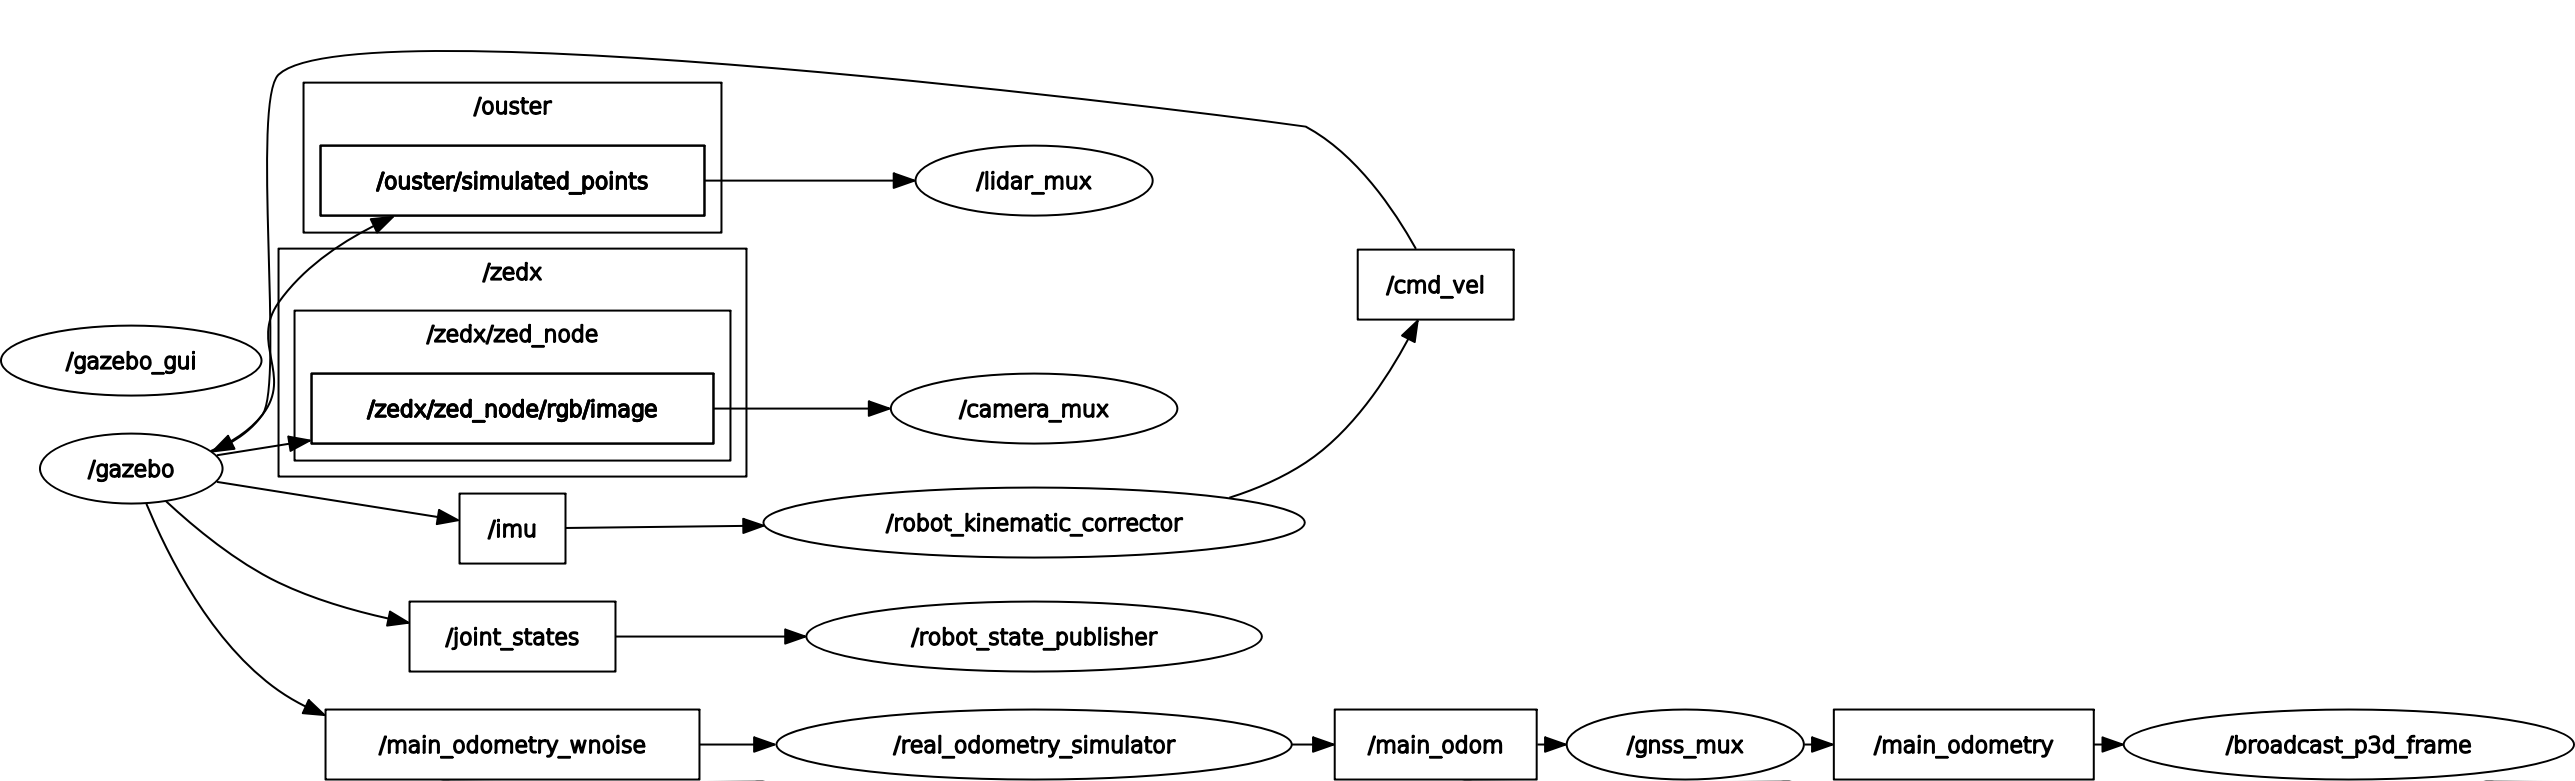
\includegraphics[scale=0.28,angle=90, origin=c]{Appendix/gazebo_sim_graph.png}
    \label{annexe1}
\end{figure}

\newpage
\section*{Annexe 2 : Checklist du rapport}
\begin{figure}[h]
    \centering
    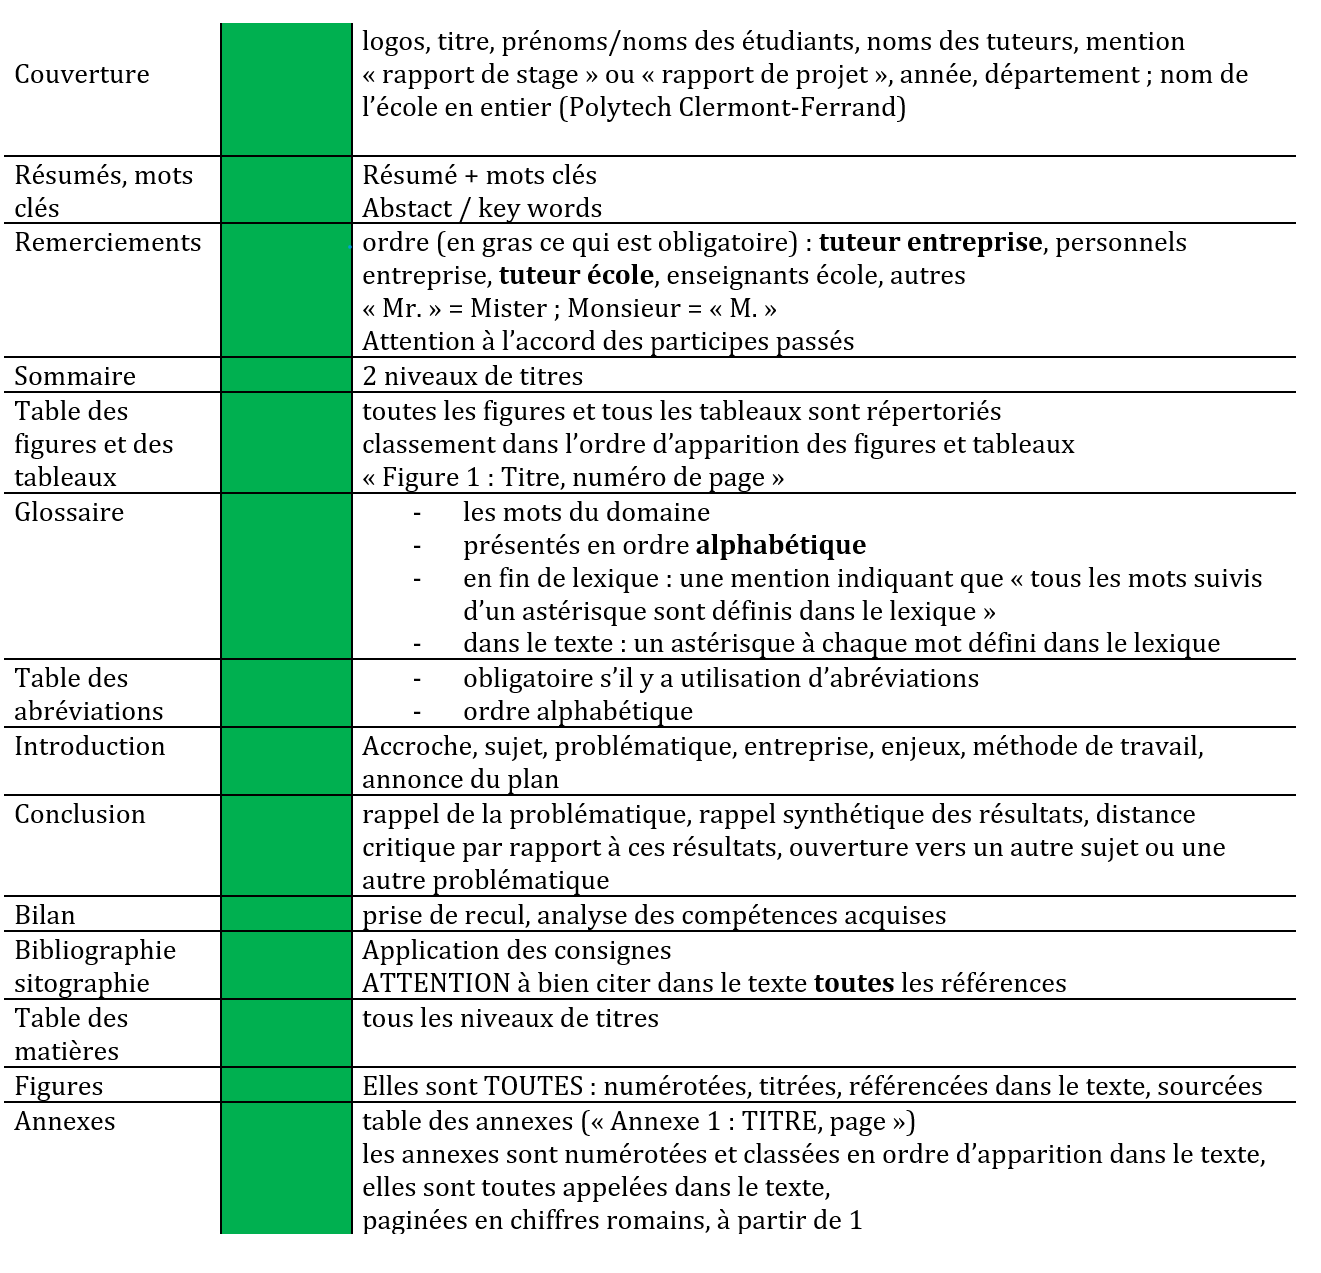
\includegraphics[width=1 \linewidth]{Appendix/checklist.png}
    \label{annexe2}
\end{figure}

\newpage
\section*{Annexe 3 : Scénario défi 3 DGA}
\label{annex3:scenarios_DGA}

\begin{center}
    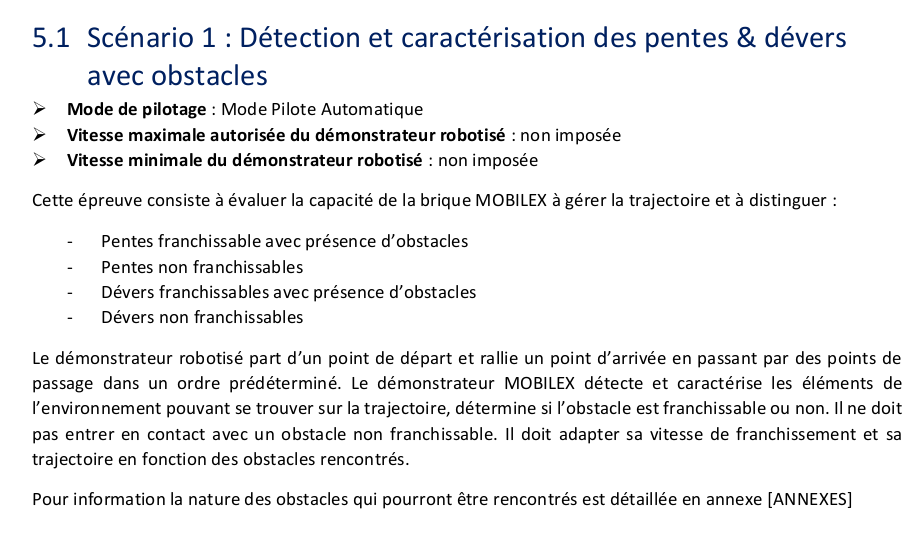
\includegraphics[width=\linewidth, height=0.45\textheight, keepaspectratio]{Appendix/scenario1.png}
\end{center}
\begin{center}
    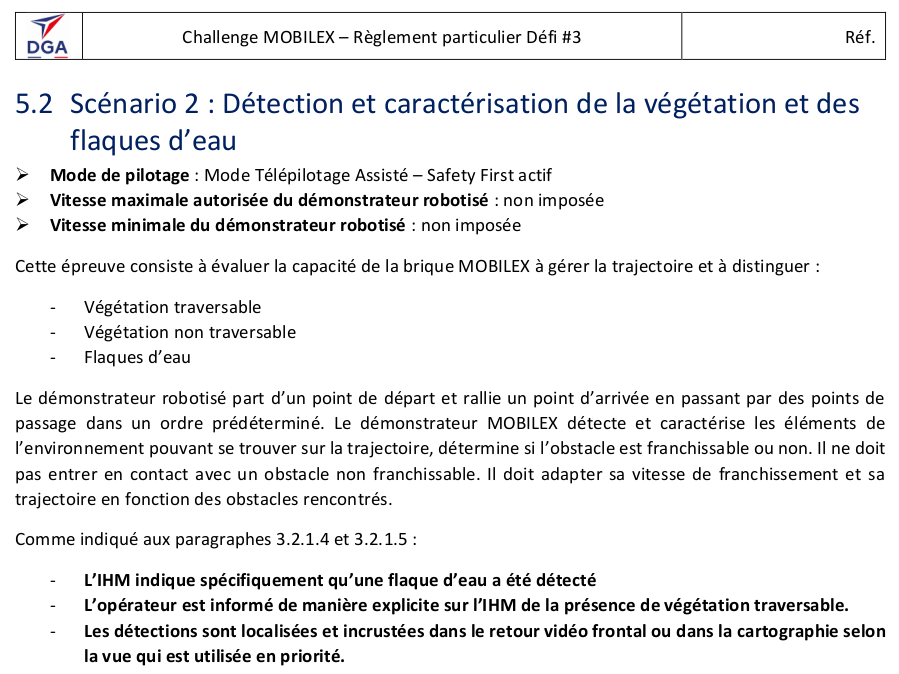
\includegraphics[width=\linewidth, height=0.5\textheight, keepaspectratio]{Appendix/scenario2.png}
\end{center}
\begin{center}
    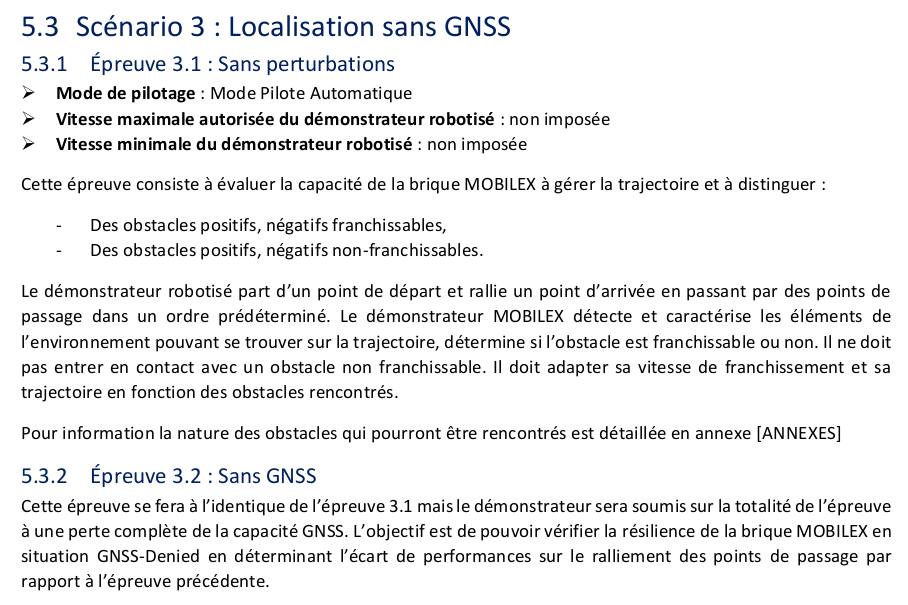
\includegraphics[width=\linewidth, height=0.45\textheight, keepaspectratio]{Appendix/scenario3.png}
\end{center}
\begin{center}
    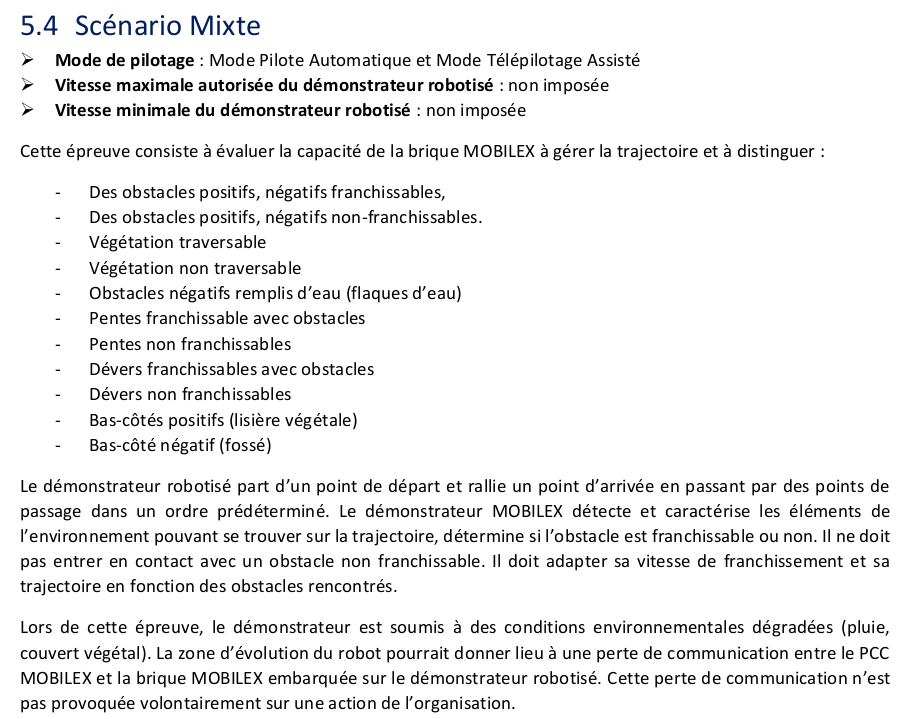
\includegraphics[width=\linewidth, height=0.5\textheight, keepaspectratio]{Appendix/scenarioM.png}
\end{center}

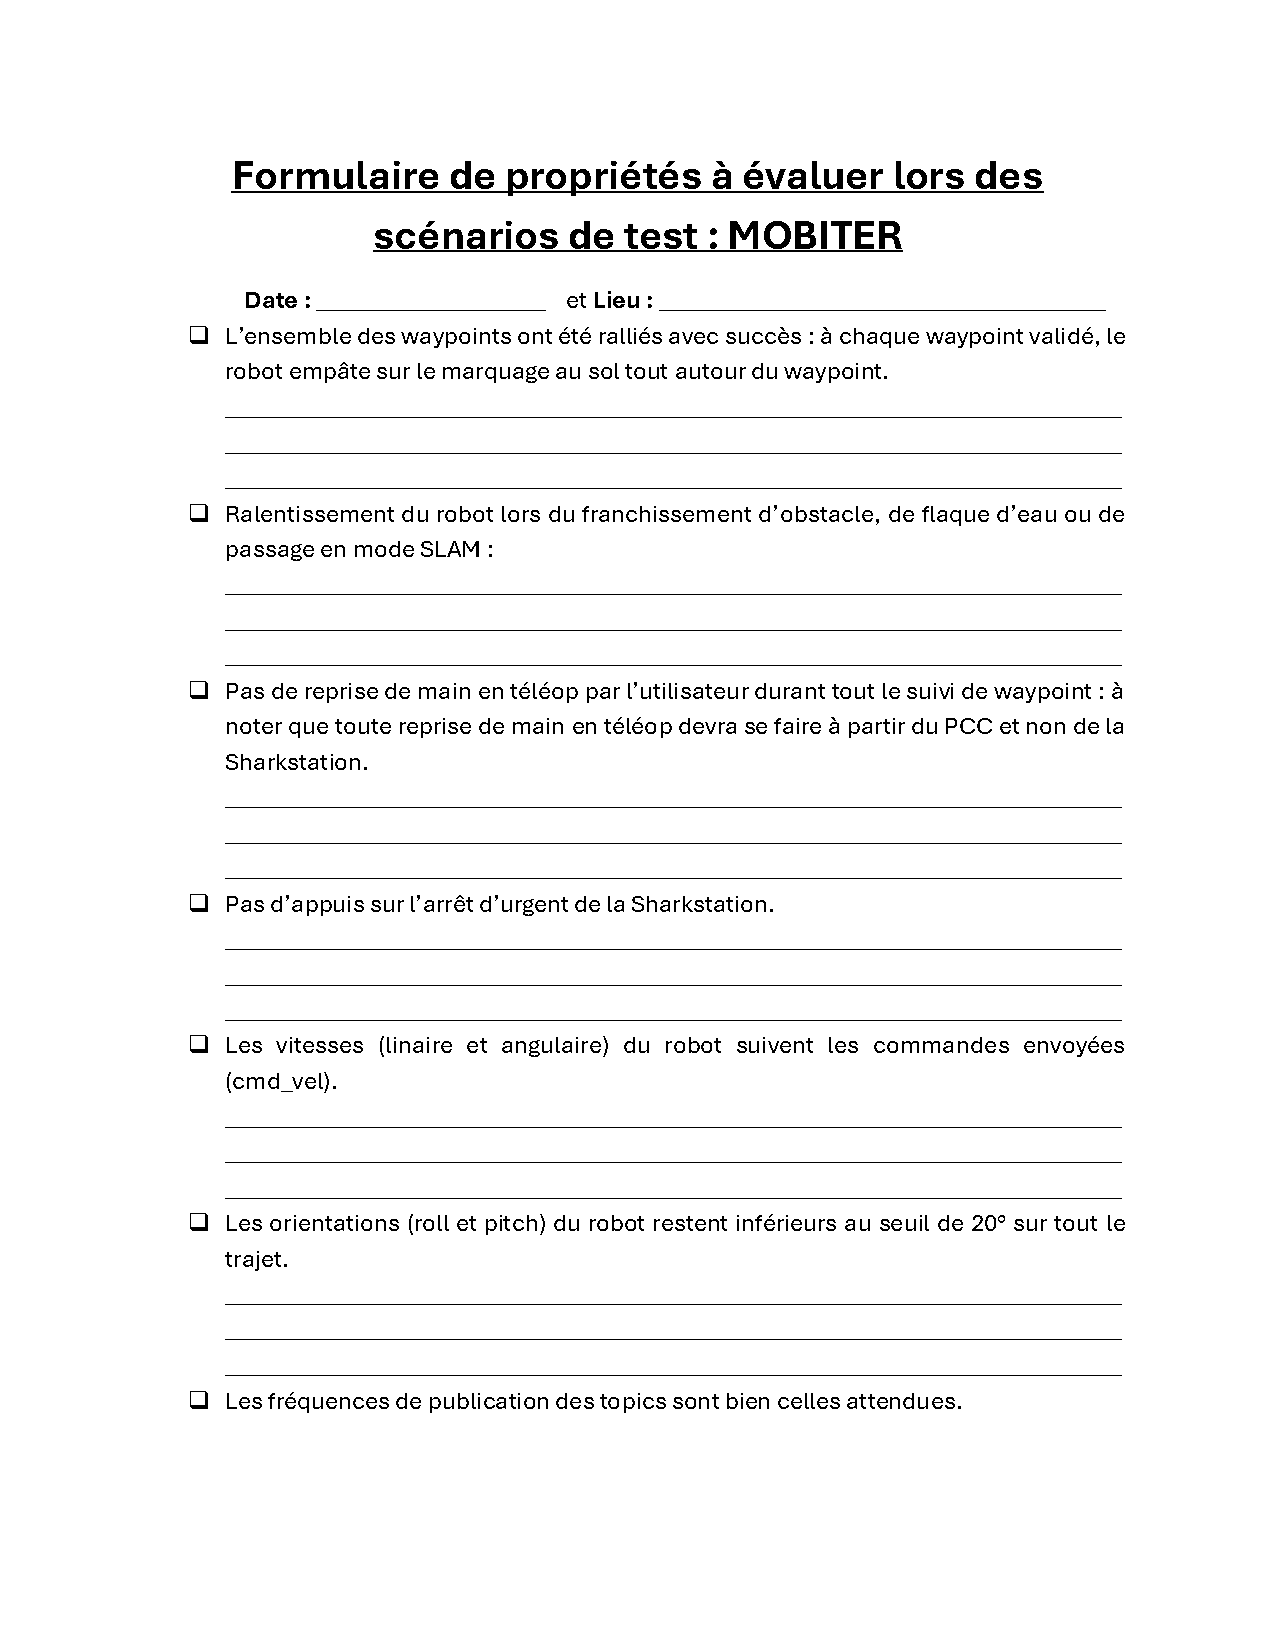
\includepdf[pages=1, pagecommand={\thispagestyle{fancy}\section*{Annexe 4 : Plan de test - Checklist}\label{annex4:test_checklist}}]{Appendix/test_checklist.pdf}
\includepdf[pages=2-]{Appendix/test_checklist.pdf}
\end{document}